\documentclass[11pt]{article}
\usepackage[margin=1in]{geometry}
\usepackage{booktabs,graphicx,longtable,tabularx,array,caption,subcaption,amsmath,hyperref,enumitem,xcolor,pdflscape}
\usepackage[T1]{fontenc}
\usepackage{lmodern}
\captionsetup{font=small,labelfont=bf}
\setlist{nosep,leftmargin=*}
\newcolumntype{L}{>{\raggedright\arraybackslash}X}
\graphicspath{{figures/}}
\emergencystretch=1.5em
\hypersetup{colorlinks=true,linkcolor=blue!60!black,citecolor=blue!60!black,urlcolor=blue!60!black}
\title{Summary Report, v5: A 100-Metric Library Calibrated on Answers of Known Quality}
\author{}
\date{2026}
\begin{document}
\maketitle

\section{Setup}

\subsection{Shared setup (identical across versions)}
\begin{itemize}
\item \textbf{Suite.} 31 datasets: 11 entity matching (EM), 6 schema matching (SM), 11 table question answering and understanding (TQA), 3 financial documents (FIN). Official test or dev splits only; 150 items per dataset by seeded stratified sampling, 100 flagged for answering (OfficeQA Pro V2: 90; Alaska schema: 93); 3,083 answered items per model. Entity-matching pools are 50/50 match / non-match (Papadakis--Christen keeps its real 1.8\,\% ratio); schema matching is one question per source column with a candidate list; BIRD is graded on the executed result of the gold SQL.
\item \textbf{Answers.} Ten models (Claude Opus 5, Claude Sonnet 5, GPT-5.5, GPT-5.4-mini, Gemini 3.8 Flash, Grok 4, DeepSeek-chat, DeepSeek-R1, gpt-oss-120b, Llama 3.3 70B); one prompt per item ending in \texttt{FINAL ANSWER: <answer>}; temperature 0 where accepted (Claude 5 and GPT-5.5 ran at provider defaults, recorded per row); output budget 700 tokens with mechanical re-asks at 2,500 and 8,000 for replies cut off before a final line; every answer cached with tokens, cost and finish reason. The same cache feeds every version, so leaderboards are directly comparable.
\item \textbf{Scoring primitives.} Extraction of the final line, Unicode / case / punctuation normalisation, number parsing with sign, percent and scale words, alias lists per gold (best alias wins), list golds, a hedge flag. Native metric per dataset: numeric tolerance (1\,\%) for numeric golds, exact match for text and boolean, ROUGE-L for free-form.
\item \textbf{Coverage rule.} A model is in the study only if it covered $\ge 90\,\%$ of the suite; a dataset counts only items every model answered and only with $\ge 20$ such items.
\item \textbf{Leaderboard machinery.} Bradley--Terry strengths from item-level pairwise wins (MLE, ridge 0.01, SE from the observed information) as the headline pooling; Borda, Kemeny (with cost), Copeland, mean-$z$, reciprocal-rank fusion and family-balanced $z$ as checks; 1,000 item bootstraps of the Borda and Bradley--Terry ranks; Friedman with Iman--Davenport, Nemenyi CD, Holm-corrected pairwise Wilcoxon across datasets; paired permutation and Wilcoxon per item within datasets (Holm); Kendall's $W$ among datasets; majority-class baselines for boolean sets; post-stratified official-split estimates with a weighted bootstrap and positive-class F1 at the official match ratio; floor / ceiling / self-stability diagnostics per dataset.
\item \textbf{Sampled designs.} Uniform-lattice, Dirichlet-snapped and Latin-hypercube samples on the weight simplex at step 0.05 (20 seeds each) with centred $L_2$ discrepancy and nearest-neighbour distances, compared with the exhaustive optimum where one exists.
\item \textbf{Reporting.} Each version's \texttt{run\_all.sh} regenerates its \texttt{REPORT.md} from the cached answers; every number in this document is read from those output files.
\end{itemize}

\subsection{What v5 searches}
\begin{itemize}
\item \textbf{Metric library.} 100 per-answer metrics in twelve families (exact-match variants, token overlap, character and sequence similarity, numeric tolerance and graded numeric error, set metrics for list golds, structure and task-specific scores, length, commitment / hedging, semantic placeholders), computed for every (model, item) pair and for every anchor.
\item \textbf{Anchors as the quality signal.} 31,380 synthetic answers generated from the golds by 20 typed operators with a known utility each (identity, verbose, tagged, unit variant = 1; paraphrase 0.95; near misses 0.75 / 0.45 / 0.15; superset 0.6; typo 0.6; partial 0.5; shuffled 0.4; hedge 0.3; list dump 0.25; digit typo 0.2; sign flip and magnitude 0.05; flip, no answer, wrong random = 0). v5 is the only version whose objective is correctness against this signal rather than agreement among the ranked models.
\item \textbf{Selection.} Drop constant metrics; cluster $|$Spearman$| \ge 0.95$ into representatives; keep candidates above an anchor-agreement floor; forward selection maximising leave-one-dataset-out Spearman of a non-negative least-squares fit to utility.
\item \textbf{Weights.} Exhaustive grid at step 0.02 over the selected weights (sum to 1) $\times$ five hedge penalties $\lambda$ (score multiplied by $1 - \lambda$ when the answer hedges): 6,630 points. Objective $J = 0.30\,\rho + 0.15\,\text{AUC} + 0.20\,(1 - \text{JS}/\ln 2) + 0.15\,\tau_{\text{native}} + 0.20\,(1 - \text{wrong mean})$, where JS is the Jensen--Shannon divergence between datasets' score distributions at matched operator (cross-dataset consistency) and $\tau_{\text{native}}$ the agreement of the composite's model ranking with the native-metric ranking. The ensemble is the mean of the 100 best weightings, so each answer carries a score and a spread.
\item \textbf{Validation.} Leave-one-dataset-out re-selection and re-fitting; utility-scale perturbation ($\pm 0.15$, five draws); gaming probes (mean score per operator vs utility against single-metric baselines); sampled designs looked up in the exhaustive grid.
\item \textbf{Leaderboards.} Exact match, the native metric, the ensemble (headline) and the five best single weightings, each pooled by Bradley--Terry with the full significance battery.
\end{itemize}

\section{Results}
\begin{table}[htbp]\centering\small\caption{v5 audit summary.}\label{tab:v5_summary}
\begin{tabularx}{\textwidth}{>{\bfseries}p{0.30\textwidth} L}\toprule
Library & 100 metrics, 10 constant on this data, 45 cluster representatives, 28 candidates above the floor \\
Selected & tok\_\allowbreak{}f1, num\_\allowbreak{}decay\_\allowbreak{}2p5, prefix\_\allowbreak{}ratio; LODO $\rho$ of the selected set 0.875 vs native typed metric alone 0.814 and exact match alone 0.831 \\
Grid & 6,630 weightings (step 0.02 $\times$ 5 $\lambda$); $J$ top-1 0.935, top-100 mean 0.933, grid median 0.923; range 0.876--0.935 \\
Ensemble weights & tok\_\allowbreak{}f1 0.17, num\_\allowbreak{}decay\_\allowbreak{}2p5 0.77, prefix\_\allowbreak{}ratio 0.06, $\lambda$ = 0.62; decay weight spans 0.54--0.96 across the top 100 \\
Ensemble terms & $\rho$ 0.904, AUC 0.996, JS 0.053, $\tau$ native 0.898, wrong mean 0.032 \\
Baselines & token F1 $\rho$ 0.859 / $J$ 0.907; numeric tolerance $\rho$ 0.806 / $J$ 0.909; ensemble $\rho$ 0.904 / $J$ 0.934 \\
Sampled designs & all three within 0.0015 of the exhaustive best (0.9348) \\
Leave-one-dataset-out & mean held-out $\rho$ 0.893 (re-fitted) vs 0.894 (full); same metric set selected in 90\,\% of folds \\
Utility perturbation & mean $L_1$ shift of the ensemble weights 0.022; selection changed in 0\,\% of draws \\
Probes (MAE to utility) & ensemble 0.116, token F1 0.144, native 0.155, exact match 0.199 \\
Leaderboard (ensemble, BT) & first Gemini 3.8 Flash ($P$(first) 0.95), then Claude Opus 5, GPT-5.5; last Llama 3.3 70B; Friedman $p$ = 2.1e-12; $W$ = 0.26 \\
Other rules & native metric: Gemini 3.8 Flash first; exact match: Claude Opus 5 first; $\tau$ ensemble vs native 0.78, vs exact match 0.87 \\
\bottomrule\end{tabularx}\end{table}

\subsection{Three metrics carry the library's information}
Of 100 metrics, 45 are distinct at $|$Spearman$| \ge 0.95$ and forward selection stops at three: token F1, numeric decay and prefix ratio (Figures~\ref{fig:fig_metric_library}, \ref{fig:fig_clusters}). Their NNLS fit reaches leave-one-dataset-out $\rho$ 0.875 against 0.814 for the native typed metric and 0.831 for exact match.
\begin{figure}[htbp]\centering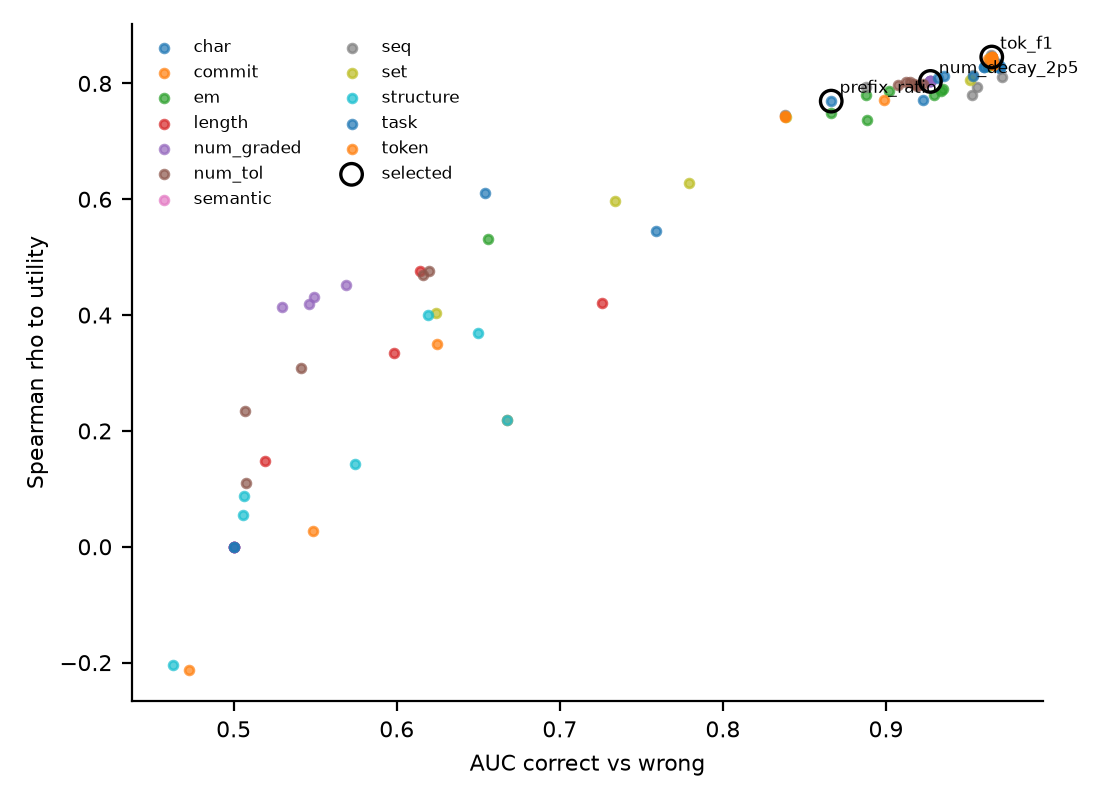
\includegraphics[width=0.7\textwidth]{fig_metric_library.png}\caption{The 100-metric library on the anchors: AUC against Spearman $\rho$, coloured by family; the three selected metrics are circled.}\label{fig:fig_metric_library}\end{figure}
\begin{figure}[htbp]\centering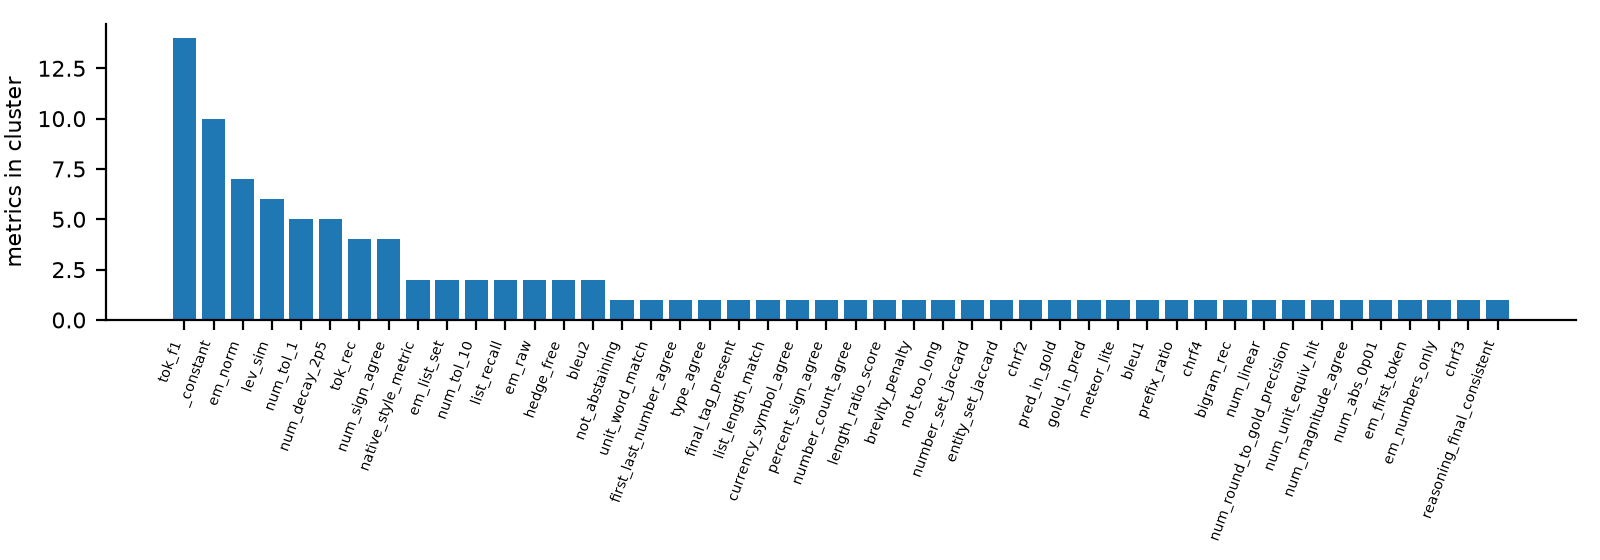
\includegraphics[width=0.85\textwidth]{fig_clusters.png}\caption{Cluster sizes after merging metrics with $|$Spearman$| \ge 0.95$ (45 representatives).}\label{fig:fig_clusters}\end{figure}
\begin{figure}[htbp]\centering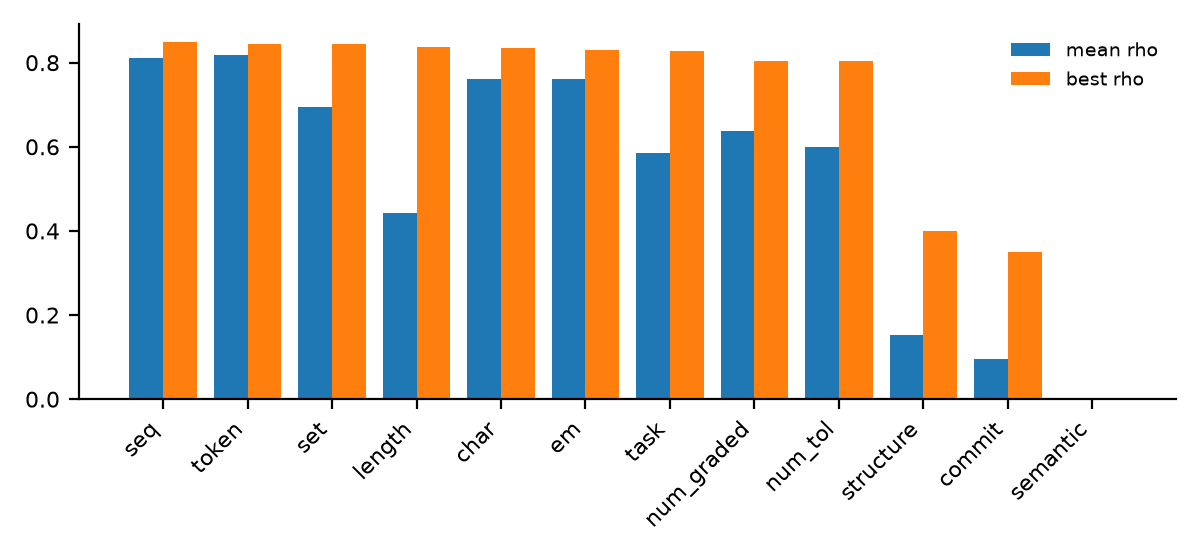
\includegraphics[width=0.7\textwidth]{fig_family_rho.png}\caption{Anchor $\rho$ per metric family: mean and best member.}\label{fig:fig_family_rho}\end{figure}


\subsection{The calibrated ensemble}
The grid is decay-dominated (Figures~\ref{fig:fig_grid_marginals}, \ref{fig:fig_top100_weights}): the top 100 put 0.77 on numeric decay with a hedge penalty of 0.62. The ensemble reaches $\rho$ 0.904 and AUC 0.996 on the anchors, above every single-metric baseline (Table~\ref{tab:baselines}, Figure~\ref{fig:fig_baselines}); the probes show where the gain comes from: near misses, unit variants and partial answers get graded credit instead of zero (Figure~\ref{fig:fig_probe_operators}, Table~\ref{tab:probes}). The sampled designs land within 0.0015 of the exhaustive best (Table~\ref{tab:designs_summary}).
\begin{figure}[htbp]\centering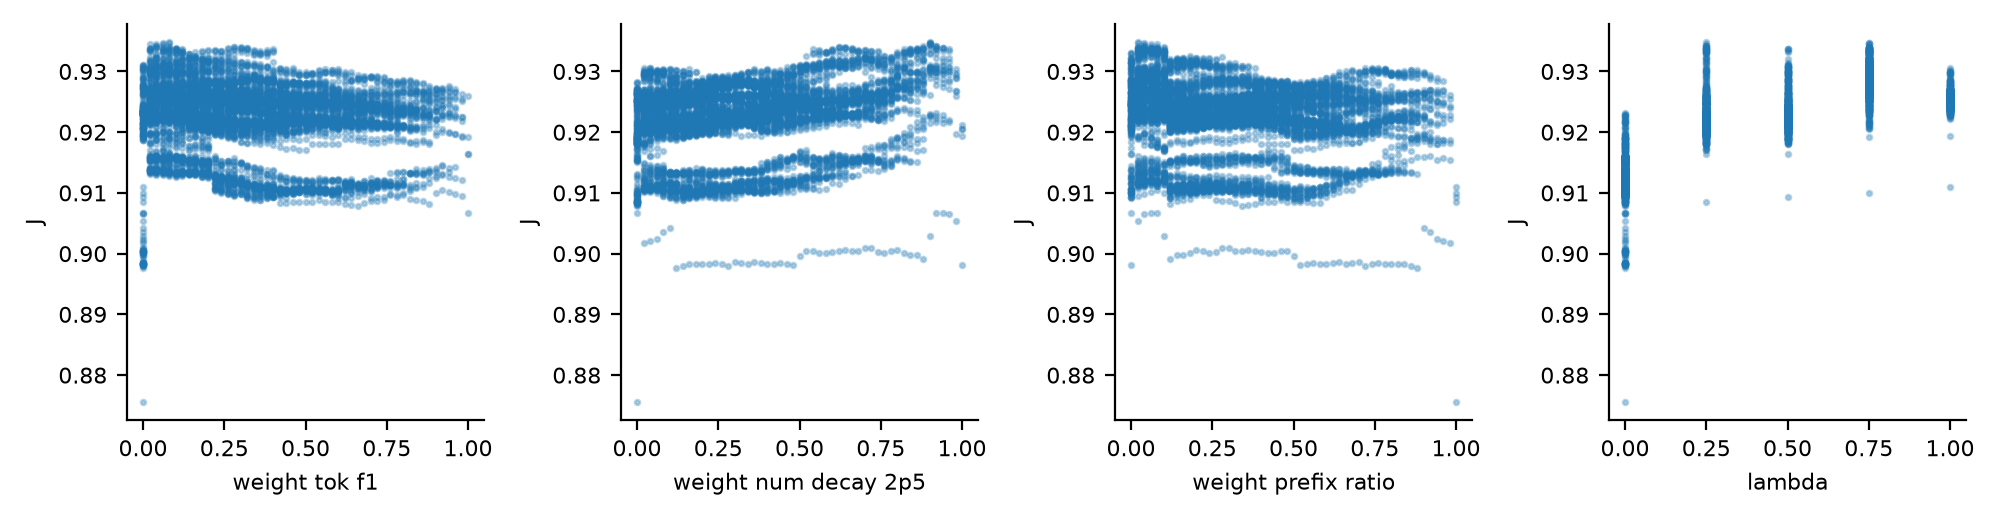
\includegraphics[width=0.85\textwidth]{fig_grid_marginals.png}\caption{Objective $J$ against each selected weight and the hedge penalty $\lambda$ over all 6,630 grid points.}\label{fig:fig_grid_marginals}\end{figure}
\begin{figure}[htbp]\centering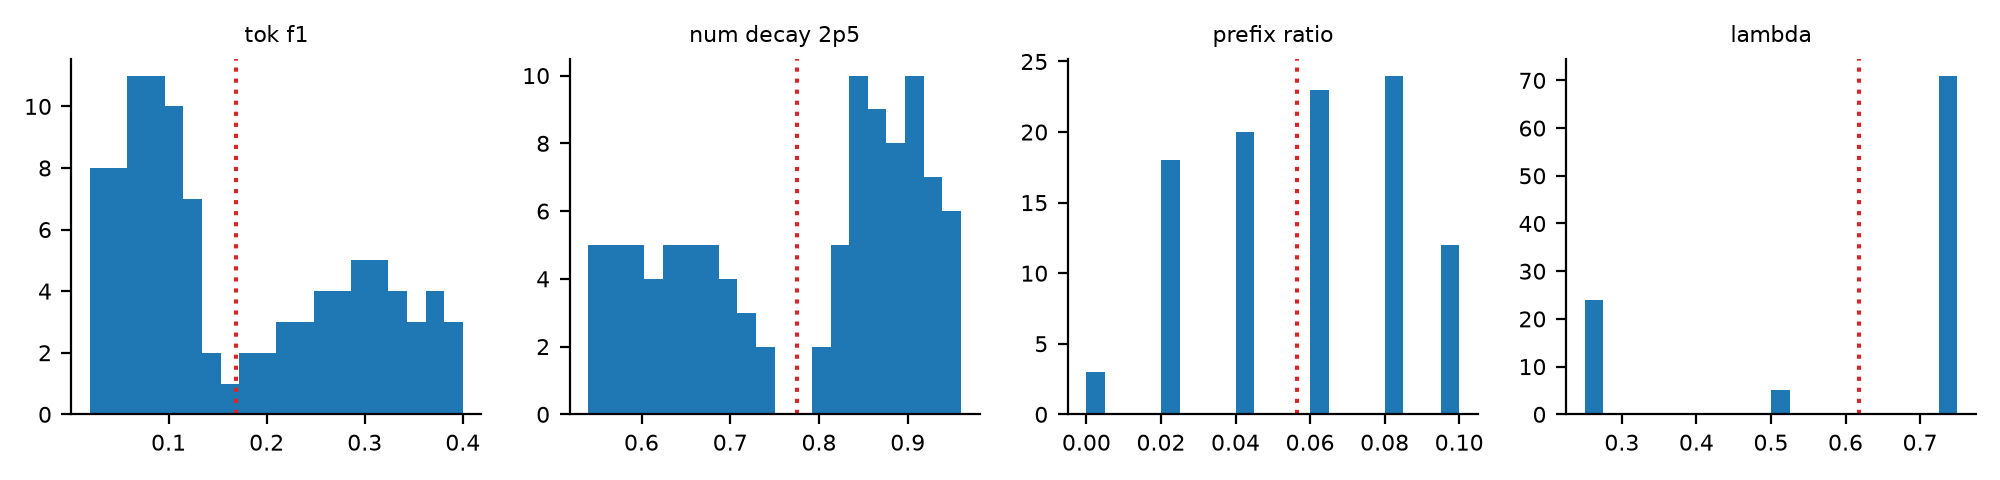
\includegraphics[width=0.85\textwidth]{fig_top100_weights.png}\caption{Weights and $\lambda$ of the 100 best grid points that form the ensemble (dotted = mean).}\label{fig:fig_top100_weights}\end{figure}
\begin{table}[htbp]
\centering\tiny
\caption{Baselines under the same objective.}
\label{tab:baselines}
\setlength{\tabcolsep}{3pt}
\begin{tabular}{p{0.572\linewidth}rrrrrr}
\toprule
baseline & rho & auc & js & bad & tau\_\allowbreak{}native & J \\
\midrule
native\_\allowbreak{}style\_\allowbreak{}metric & 0.826 & 0.935 & 0.031 & 0.014 & 0.992 & 0.925 \\
em\_\allowbreak{}norm & 0.849 & 0.963 & 0.024 & 0.012 & 0.924 & 0.928 \\
tok\_\allowbreak{}f1 & 0.859 & 0.965 & 0.079 & 0.032 & 0.888 & 0.907 \\
rouge\_\allowbreak{}l & 0.862 & 0.965 & 0.082 & 0.032 & 0.892 & 0.907 \\
num\_\allowbreak{}tol\_\allowbreak{}1 & 0.806 & 0.919 & 0.032 & 0.016 & 0.946 & 0.909 \\
uniform\_\allowbreak{}over\_\allowbreak{}selected\_\allowbreak{}no\_\allowbreak{}gate & 0.882 & 0.970 & 0.098 & 0.028 & 0.900 & 0.911 \\
ensemble\_\allowbreak{}top100 & 0.904 & 0.996 & 0.053 & 0.032 & 0.898 & 0.934 \\
\bottomrule
\end{tabular}
\end{table}

\begin{figure}[htbp]\centering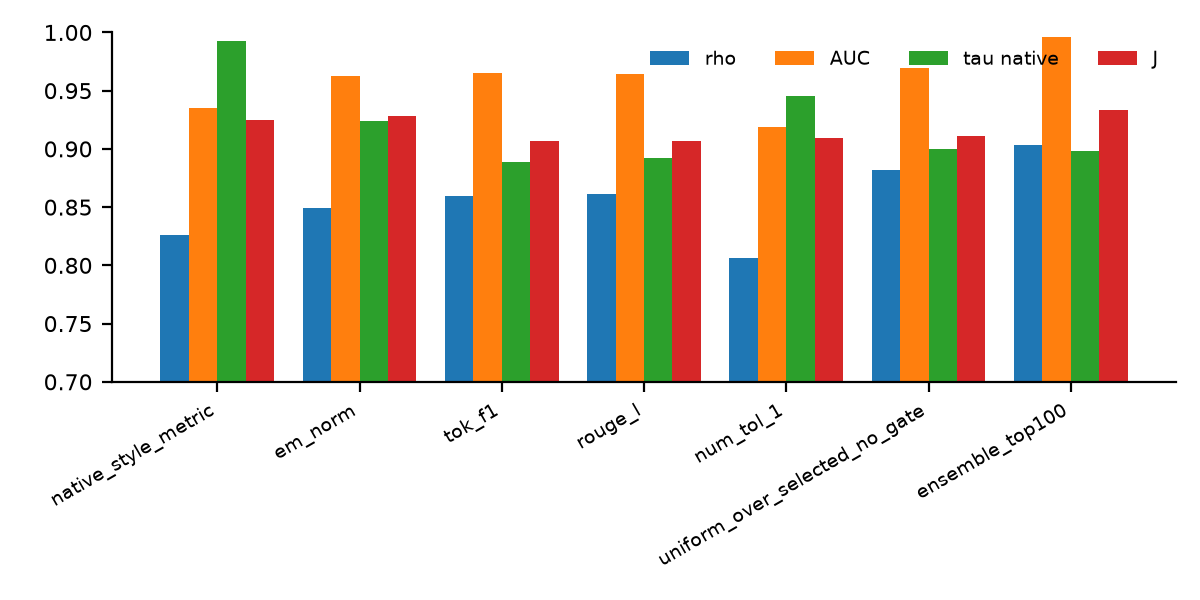
\includegraphics[width=0.7\textwidth]{fig_baselines.png}\caption{Single-metric baselines against the ensemble under the same objective terms.}\label{fig:fig_baselines}\end{figure}
\begin{figure}[htbp]\centering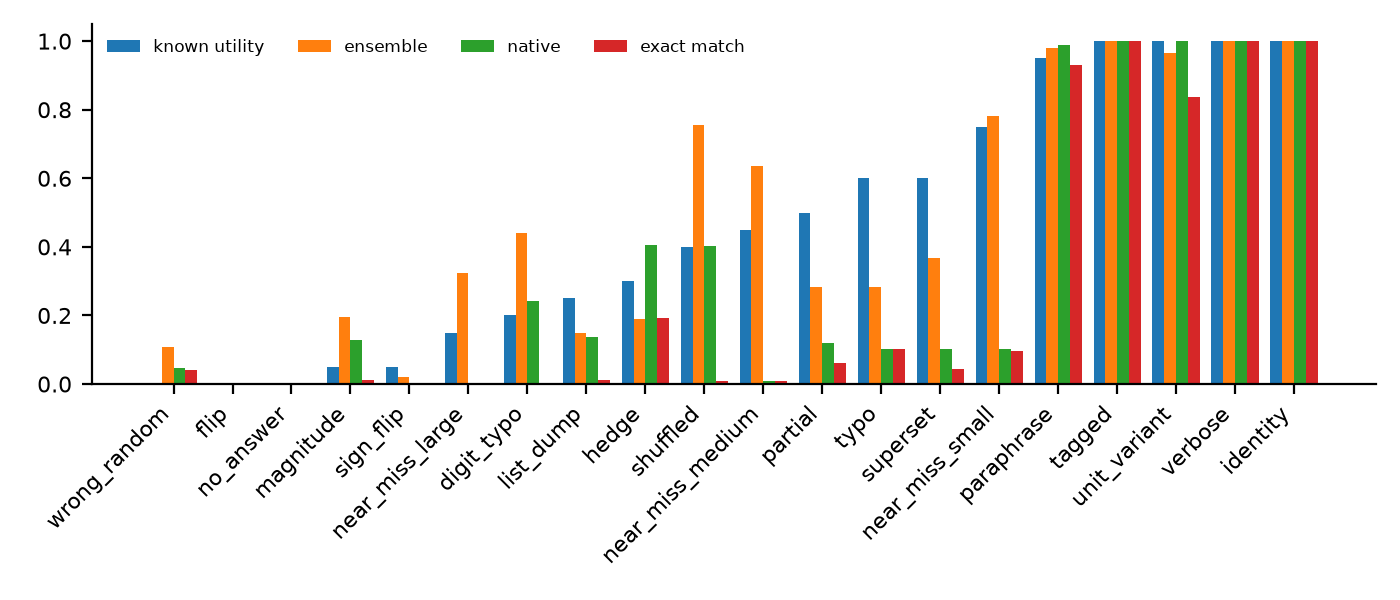
\includegraphics[width=0.85\textwidth]{fig_probe_operators.png}\caption{Mean score per anchor operator under the ensemble, the native metric and exact match, against known utility.}\label{fig:fig_probe_operators}\end{figure}
\begin{table}[htbp]
\centering\tiny
\caption{Sampled designs vs the exhaustive grid (best $J$ = 0.9348 over 6630 points).}
\label{tab:designs_summary}
\setlength{\tabcolsep}{3pt}
\begin{tabular}{p{0.185\linewidth}p{0.120\linewidth}rp{0.120\linewidth}rp{0.163\linewidth}p{0.120\linewidth}r}
\toprule
design & best\_\allowbreak{}J\_\allowbreak{}mean & best\_\allowbreak{}J\_\allowbreak{}sd & regret\_\allowbreak{}mean & regret\_\allowbreak{}max & min\_\allowbreak{}pairwise\_\allowbreak{}L1 & discrepancy & zero\_\allowbreak{}share \\
\midrule
dirichlet\_\allowbreak{}lattice & 0.9342 & 0.0004 & 0.0007 & 0.0014 & 0.0400 & 0.2728 & 0.0615 \\
lhs\_\allowbreak{}simplex & 0.9340 & 0.0003 & 0.0008 & 0.0015 & 0.0400 & 0.2702 & 0.0555 \\
uniform\_\allowbreak{}lattice & 0.9342 & 0.0003 & 0.0007 & 0.0014 & 0.0400 & 0.2639 & 0.1115 \\
\bottomrule
\end{tabular}
\end{table}



\subsection{Validation}
Leaving any dataset out re-selects the same three metrics in 90\,\% of folds and changes held-out $\rho$ by 0.001 on average (Figure~\ref{fig:fig_lodo}); perturbing the utility scale by $\pm 0.15$ moves the weights by 0.022 in $L_1$ and never changes the selection. The hand-set utility scale is the main assumption, and these checks say the result is not sensitive to it.
\begin{figure}[htbp]\centering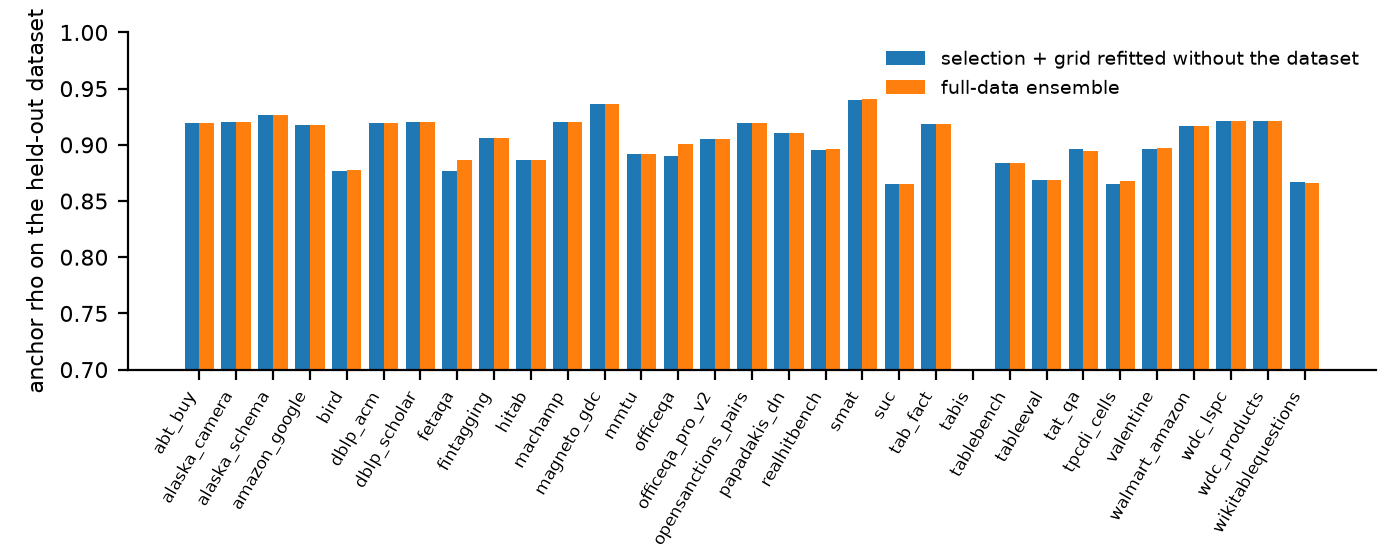
\includegraphics[width=0.85\textwidth]{fig_lodo.png}\caption{Leave-one-dataset-out: anchor $\rho$ on the held-out dataset under the re-fitted and the full-data ensemble.}\label{fig:fig_lodo}\end{figure}
\begin{table}[htbp]
\centering\scriptsize
\caption{Validation summary.}
\label{tab:validation}
\setlength{\tabcolsep}{3pt}
\begin{tabular}{p{0.892\linewidth}r}
\toprule
quantity & value \\
\midrule
lodo\_\allowbreak{}mean\_\allowbreak{}rho\_\allowbreak{}lodo & 0.8934 \\
lodo\_\allowbreak{}mean\_\allowbreak{}rho\_\allowbreak{}full & 0.8942 \\
lodo\_\allowbreak{}same\_\allowbreak{}selection\_\allowbreak{}share & 0.9032 \\
severity\_\allowbreak{}l1\_\allowbreak{}shift\_\allowbreak{}mean & 0.0220 \\
severity\_\allowbreak{}l1\_\allowbreak{}shift\_\allowbreak{}max & 0.0220 \\
severity\_\allowbreak{}selection\_\allowbreak{}changed\_\allowbreak{}share & 0.0000 \\
probe\_\allowbreak{}mae\_\allowbreak{}ensemble & 0.1158 \\
probe\_\allowbreak{}mae\_\allowbreak{}em & 0.1991 \\
probe\_\allowbreak{}mae\_\allowbreak{}native & 0.1545 \\
probe\_\allowbreak{}mae\_\allowbreak{}tok\_\allowbreak{}f1 & 0.1440 \\
\bottomrule
\end{tabular}
\end{table}



\subsection{Leaderboard}
Under the ensemble pooled by Bradley--Terry, Gemini 3.8 Flash is first, Claude Opus 5 and GPT-5.5 next, Llama 3.3 70B last; Borda puts Claude Opus 5 first. The five best single weightings give the same ranking as the ensemble ($\tau$ = 1.00); the native metric and exact match move the top three. Dataset agreement stays moderate ($W$ = 0.26). The ensemble spread per answer (Figure~\ref{fig:fig_ensemble_spread}) is largest on the free-form and list datasets, which is where the weighting matters.
\begin{table}[htbp]
\centering\tiny
\caption{Leaderboard under the headline rule (ensemble).}
\label{tab:leaderboard_headline}
\setlength{\tabcolsep}{3pt}
\begin{tabular}{lp{0.256\linewidth}p{0.176\linewidth}rrrp{0.176\linewidth}r}
\toprule
rank & model & BT strength & SE & Borda rank & Borda 95\% & P(first) BT & mean score \\
\midrule
1 & Gemini 3.8 Flash & 0.128 & 0.016 & 3 & [1, 3] & 0.950 & 0.835 \\
2 & Claude Opus 5 & 0.110 & 0.000 & 1 & [1, 3] & 0.050 & 0.833 \\
3 & GPT-5.5 & 0.047 & 0.016 & 2 & [1, 3] & 0.000 & 0.824 \\
4 & Claude Sonnet 5 & 0.035 & 0.016 & 4 & [4, 6] & 0.000 & 0.814 \\
5 & Grok 4 & 0.026 & 0.016 & 5 & [4, 7] & 0.000 & 0.811 \\
6 & GPT-5.4-mini & -0.009 & 0.016 & 6 & [4, 8] & 0.000 & 0.805 \\
7 & DeepSeek-chat & -0.020 & 0.016 & 8 & [5, 8] & 0.000 & 0.798 \\
8 & DeepSeek-R1 & -0.050 & 0.016 & 7 & [5, 8] & 0.000 & 0.794 \\
9 & gpt-oss-120b & -0.089 & 0.016 & 9 & [9, 10] & 0.000 & 0.784 \\
10 & Llama 3.3 70B & -0.177 & 0.016 & 10 & [9, 10] & 0.000 & 0.747 \\
\bottomrule
\end{tabular}
\end{table}

\begin{landscape}
\begin{table}[htbp]
\centering\tiny
\caption{Bradley--Terry rank (Borda rank in brackets) under each reported rule, Friedman $p$ and Kendall's $W$ among datasets.}
\label{tab:ranks_by_rule}
\setlength{\tabcolsep}{3pt}
\resizebox{\linewidth}{!}{%
\begin{tabular}{lrrrrrrrrrrrr}
\toprule
rule & Gemini 3.8 Flash & Claude Opus 5 & GPT-5.5 & Claude Sonnet 5 & Grok 4 & GPT-5.4-mini & DeepSeek-chat & DeepSeek-R1 & gpt-oss-120b & Llama 3.3 70B & Friedman p & W \\
\midrule
exact match & 2 (3) & 1 (1) & 3 (2) & 5 (4) & 4 (5) & 6 (8) & 8 (7) & 7 (6) & 9 (9) & 10 (10) & 2.7e-14 & 0.28 \\
native metric & 1 (3) & 3 (2) & 2 (1) & 5 (4) & 4 (5) & 8 (7) & 7 (8) & 6 (6) & 9 (9) & 10 (10) & 3.8e-14 & 0.28 \\
ensemble & 1 (3) & 2 (1) & 3 (2) & 4 (4) & 5 (5) & 6 (6) & 7 (8) & 8 (7) & 9 (9) & 10 (10) & 2.1e-12 & 0.26 \\
top1 & 1 (3) & 2 (1) & 3 (2) & 4 (4) & 5 (5) & 6 (6) & 7 (8) & 8 (7) & 9 (9) & 10 (10) & 2.9e-12 & 0.26 \\
top2 & 1 (3) & 2 (1) & 3 (2) & 4 (4) & 5 (5) & 6 (6) & 7 (8) & 8 (7) & 9 (9) & 10 (10) & 2.2e-12 & 0.26 \\
top3 & 1 (3) & 2 (1) & 3 (2) & 4 (4) & 5 (5) & 6 (6) & 7 (8) & 8 (7) & 9 (9) & 10 (10) & 2.7e-12 & 0.26 \\
top4 & 1 (3) & 2 (1) & 3 (2) & 4 (4) & 5 (5) & 6 (6) & 7 (8) & 8 (7) & 9 (9) & 10 (10) & 3.6e-12 & 0.25 \\
top5 & 1 (3) & 2 (1) & 3 (2) & 4 (4) & 5 (5) & 6 (6) & 7 (8) & 8 (7) & 9 (9) & 10 (10) & 4.2e-12 & 0.25 \\
\bottomrule
\end{tabular}
}
\end{table}
\end{landscape}

\begin{figure}[htbp]\centering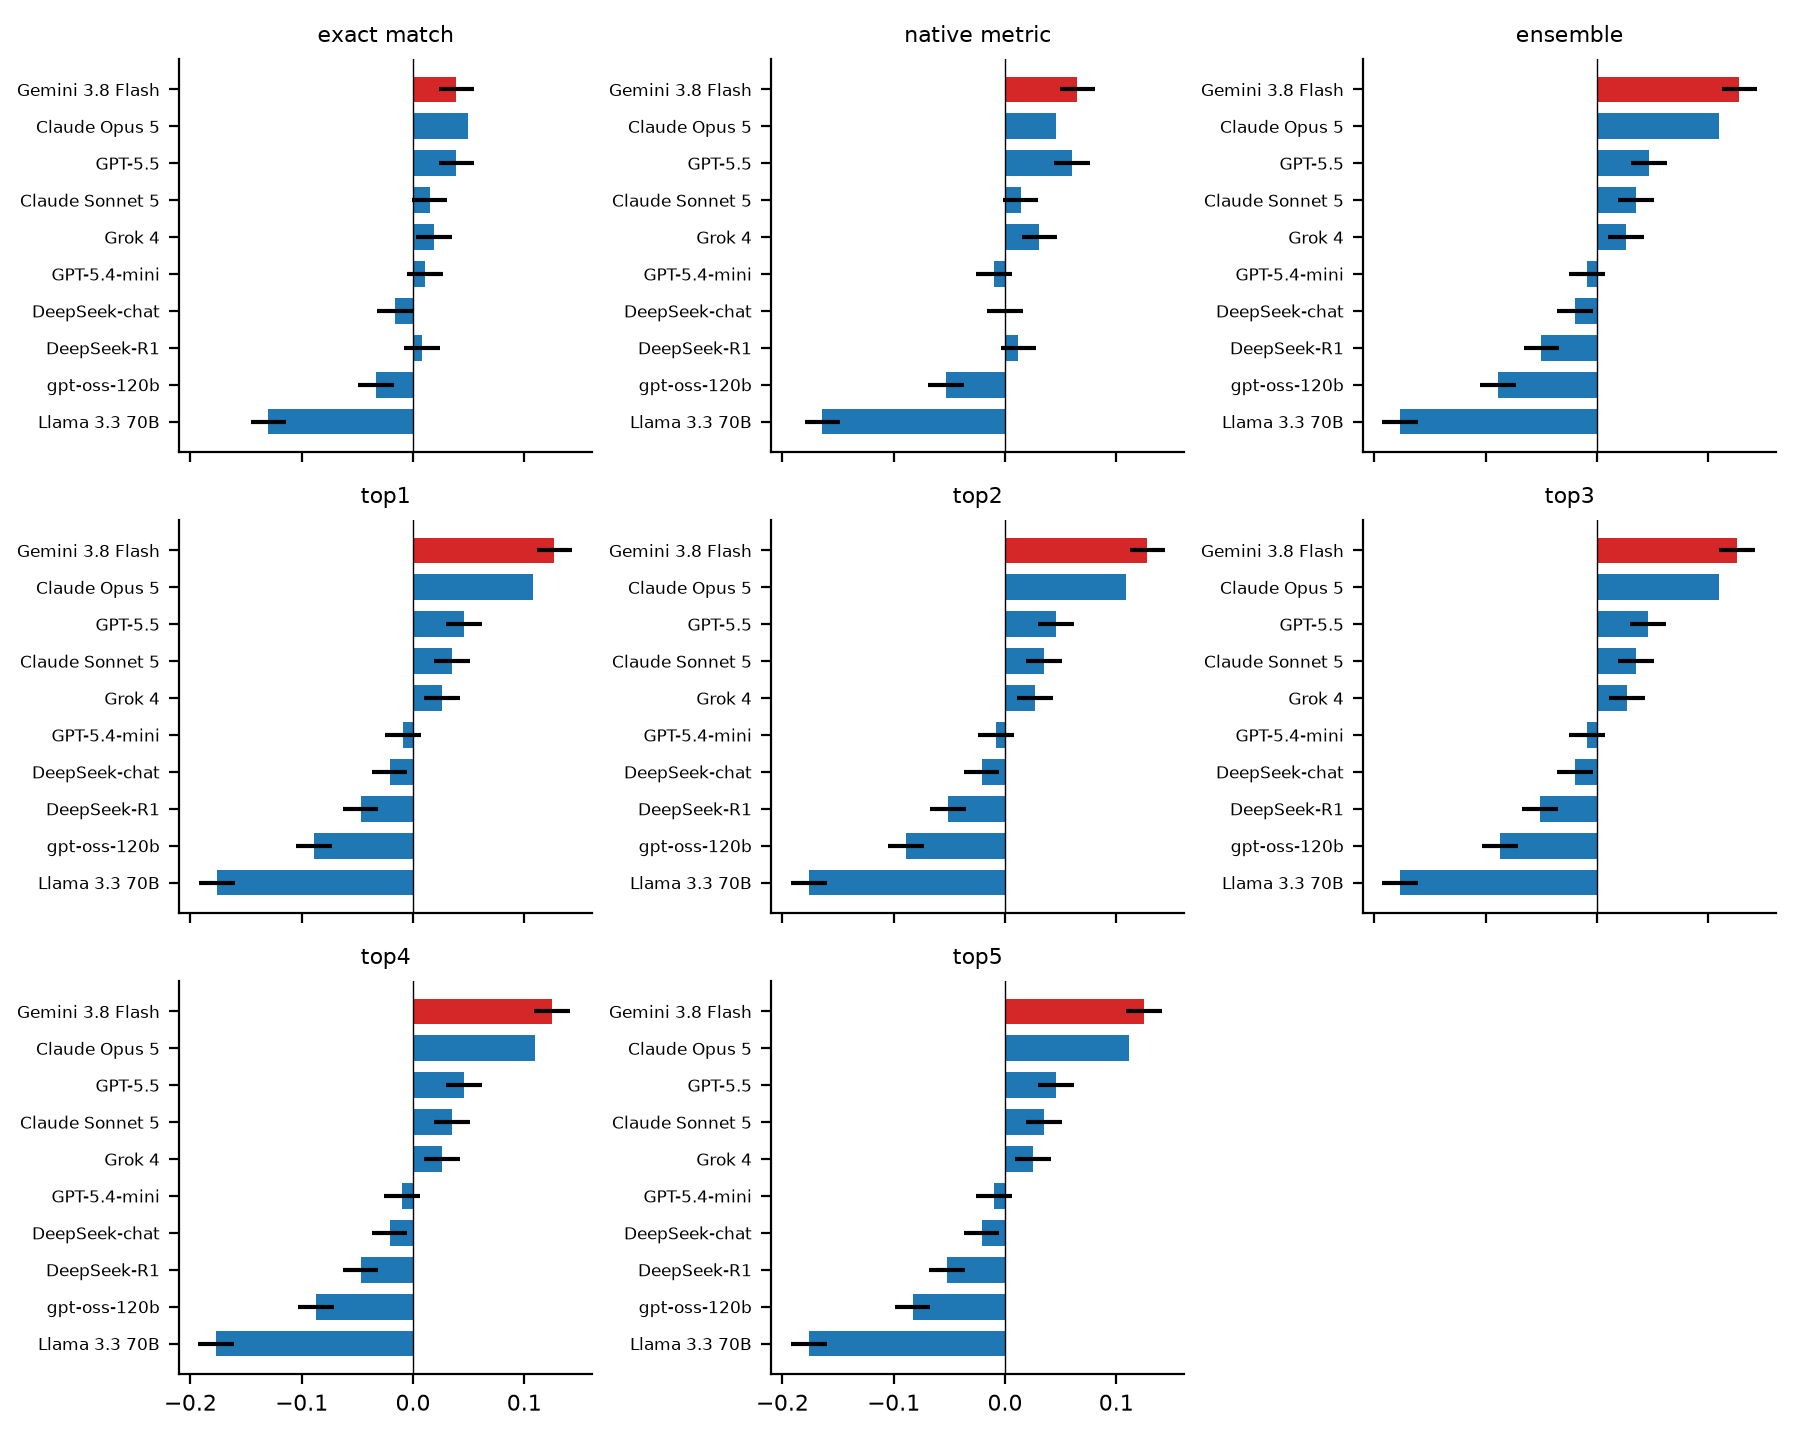
\includegraphics[width=0.85\textwidth]{fig_bt_all_rules.png}\caption{Bradley--Terry strengths ($\pm$ SE vs reference) under every reported rule; models fixed in the headline order.}\label{fig:fig_bt_all_rules}\end{figure}
\begin{figure}[htbp]\centering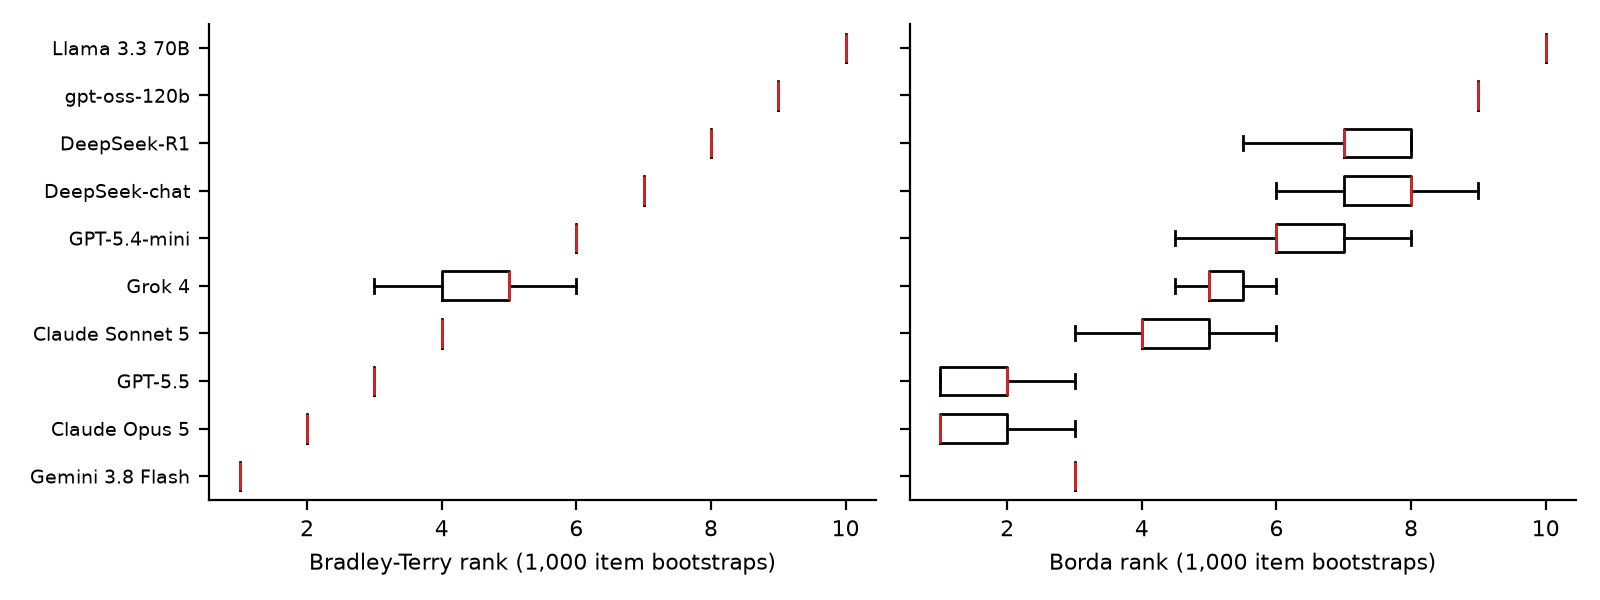
\includegraphics[width=0.85\textwidth]{fig_rank_bootstrap.png}\caption{Bootstrap distribution of each model's rank under the headline rule (ensemble).}\label{fig:fig_rank_bootstrap}\end{figure}
\begin{figure}[htbp]\centering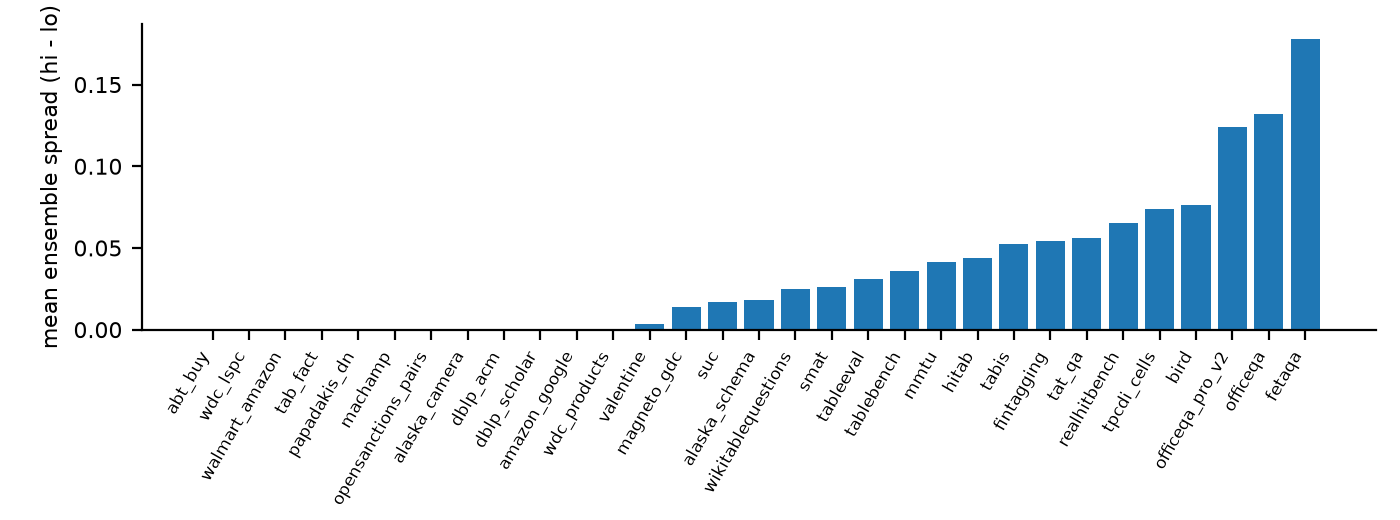
\includegraphics[width=0.85\textwidth]{fig_ensemble_spread.png}\caption{Ensemble uncertainty per dataset: mean spread of the per-answer score across the 100 weightings.}\label{fig:fig_ensemble_spread}\end{figure}


\subsection{Comparability and diagnostics}
\begin{table}[htbp]
\centering\tiny
\caption{Official-split estimates under the headline rule averaged over the ten models.}
\label{tab:official_split_by_dataset}
\setlength{\tabcolsep}{3pt}
\begin{tabular}{p{0.121\linewidth}rp{0.108\linewidth}p{0.076\linewidth}p{0.140\linewidth}p{0.121\linewidth}p{0.095\linewidth}p{0.146\linewidth}}
\toprule
dataset & suite\_\allowbreak{}mean & official\_\allowbreak{}estimate & suite\_\allowbreak{}f1\_\allowbreak{}pos & official\_\allowbreak{}precision\_\allowbreak{}pos & official\_\allowbreak{}recall\_\allowbreak{}pos & official\_\allowbreak{}f1\_\allowbreak{}pos & official\_\allowbreak{}positive\_\allowbreak{}share \\
\midrule
abt\_\allowbreak{}buy & 0.970 & 0.986 & 0.968 & 0.926 & 0.949 & 0.936 & 0.108 \\
alaska\_\allowbreak{}camera & 0.958 & 0.958 & 0.955 & 1.000 & 0.921 & 0.955 & 0.500 \\
alaska\_\allowbreak{}schema & 0.909 & 0.909 & -- & -- & -- & -- & -- \\
amazon\_\allowbreak{}google & 0.935 & 0.932 & 0.928 & 0.611 & 0.941 & 0.739 & 0.102 \\
bird & 0.252 & 0.271 & -- & -- & -- & -- & -- \\
dblp\_\allowbreak{}acm & 0.986 & 0.991 & 0.985 & 0.979 & 0.978 & 0.976 & 0.180 \\
dblp\_\allowbreak{}scholar & 0.949 & 0.966 & 0.948 & 0.900 & 0.924 & 0.910 & 0.186 \\
fetaqa & 0.559 & 0.559 & -- & -- & -- & -- & -- \\
fintagging & 0.823 & 0.821 & -- & -- & -- & -- & -- \\
hitab & 0.775 & 0.788 & -- & -- & -- & -- & -- \\
machamp & 0.887 & 0.890 & 0.892 & 0.644 & 0.853 & 0.733 & 0.175 \\
magneto\_\allowbreak{}gdc & 0.915 & 0.919 & -- & -- & -- & -- & -- \\
mmtu & 0.862 & 0.810 & -- & -- & -- & -- & -- \\
officeqa & 0.273 & 0.273 & -- & -- & -- & -- & -- \\
officeqa\_\allowbreak{}pro\_\allowbreak{}v2 & 0.294 & 0.294 & -- & -- & -- & -- & -- \\
opensanctions\_\allowbreak{}pairs & 0.821 & 0.727 & 0.773 & 0.993 & 0.649 & 0.777 & 0.769 \\
papadakis\_\allowbreak{}dn & 0.941 & 0.988 & 0.833 & 0.550 & 0.963 & 0.683 & 0.018 \\
realhitbench & 0.717 & 0.716 & -- & -- & -- & -- & -- \\
smat & 0.890 & 0.887 & -- & -- & -- & -- & -- \\
suc & 0.950 & 0.950 & -- & -- & -- & -- & -- \\
tab\_\allowbreak{}fact & 0.798 & 0.789 & 0.758 & 0.896 & 0.674 & 0.764 & 0.500 \\
tabis & 0.885 & 0.889 & -- & -- & -- & -- & -- \\
tablebench & 0.854 & 0.860 & -- & -- & -- & -- & -- \\
tableeval & 0.771 & 0.776 & -- & -- & -- & -- & -- \\
tat\_\allowbreak{}qa & 0.797 & 0.755 & -- & -- & -- & -- & -- \\
tpcdi\_\allowbreak{}cells & 0.418 & 0.450 & -- & -- & -- & -- & -- \\
valentine & 0.981 & 0.974 & -- & -- & -- & -- & -- \\
walmart\_\allowbreak{}amazon & 0.958 & 0.975 & 0.947 & 0.832 & 0.927 & 0.875 & 0.094 \\
wdc\_\allowbreak{}lspc & 0.982 & 0.983 & 0.983 & 0.965 & 0.979 & 0.971 & 0.264 \\
wdc\_\allowbreak{}products & 0.977 & 0.985 & 0.979 & 0.980 & 0.967 & 0.973 & 0.280 \\
wikitablequestions & 0.850 & 0.849 & -- & -- & -- & -- & -- \\
\bottomrule
\end{tabular}
\end{table}

\begin{figure}[htbp]\centering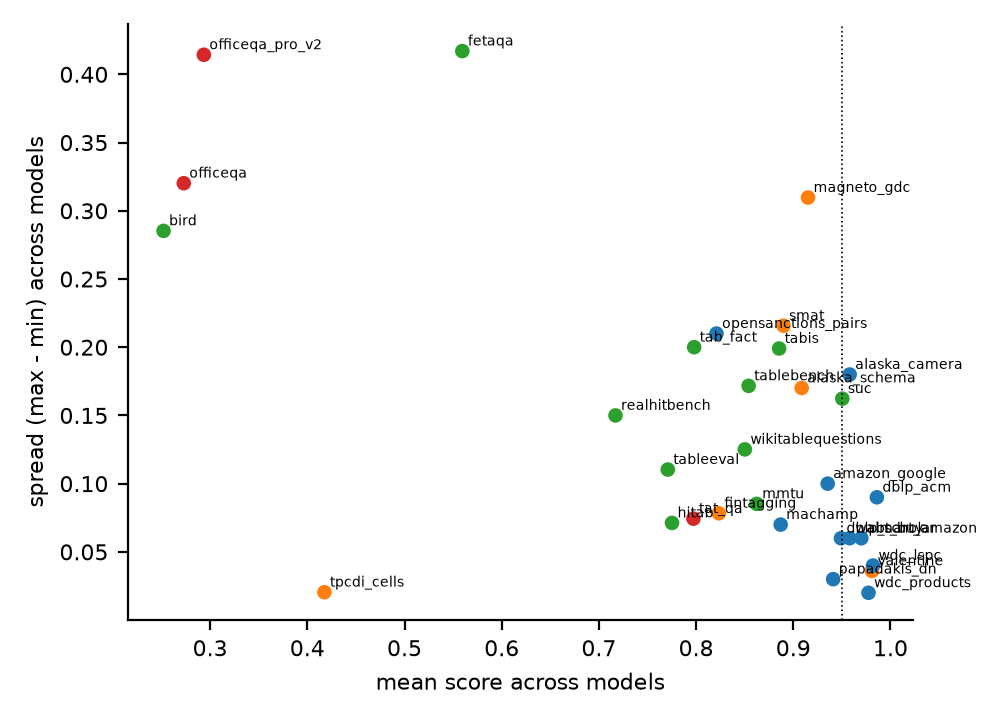
\includegraphics[width=0.6\textwidth]{fig_diagnostics_scatter.png}\caption{Dataset diagnostics: mean score against spread across models; dotted line marks the ceiling flag.}\label{fig:fig_diagnostics_scatter}\end{figure}


\clearpage
\appendix
\section{All figures}
Every figure that can be drawn from the saved outputs; source data in \texttt{data/}.
\begin{figure}[htbp]\centering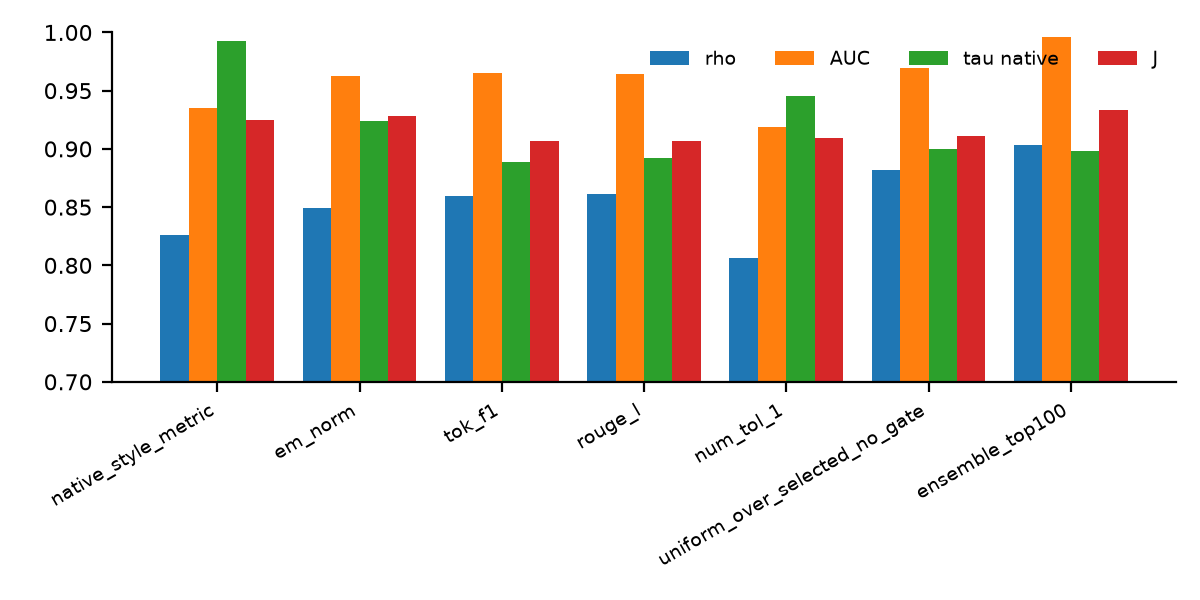
\includegraphics[width=0.9\textwidth]{fig_baselines.png}\caption{Single-metric baselines against the ensemble under the same objective terms.}\label{figall:fig_baselines}\end{figure}
\begin{figure}[htbp]\centering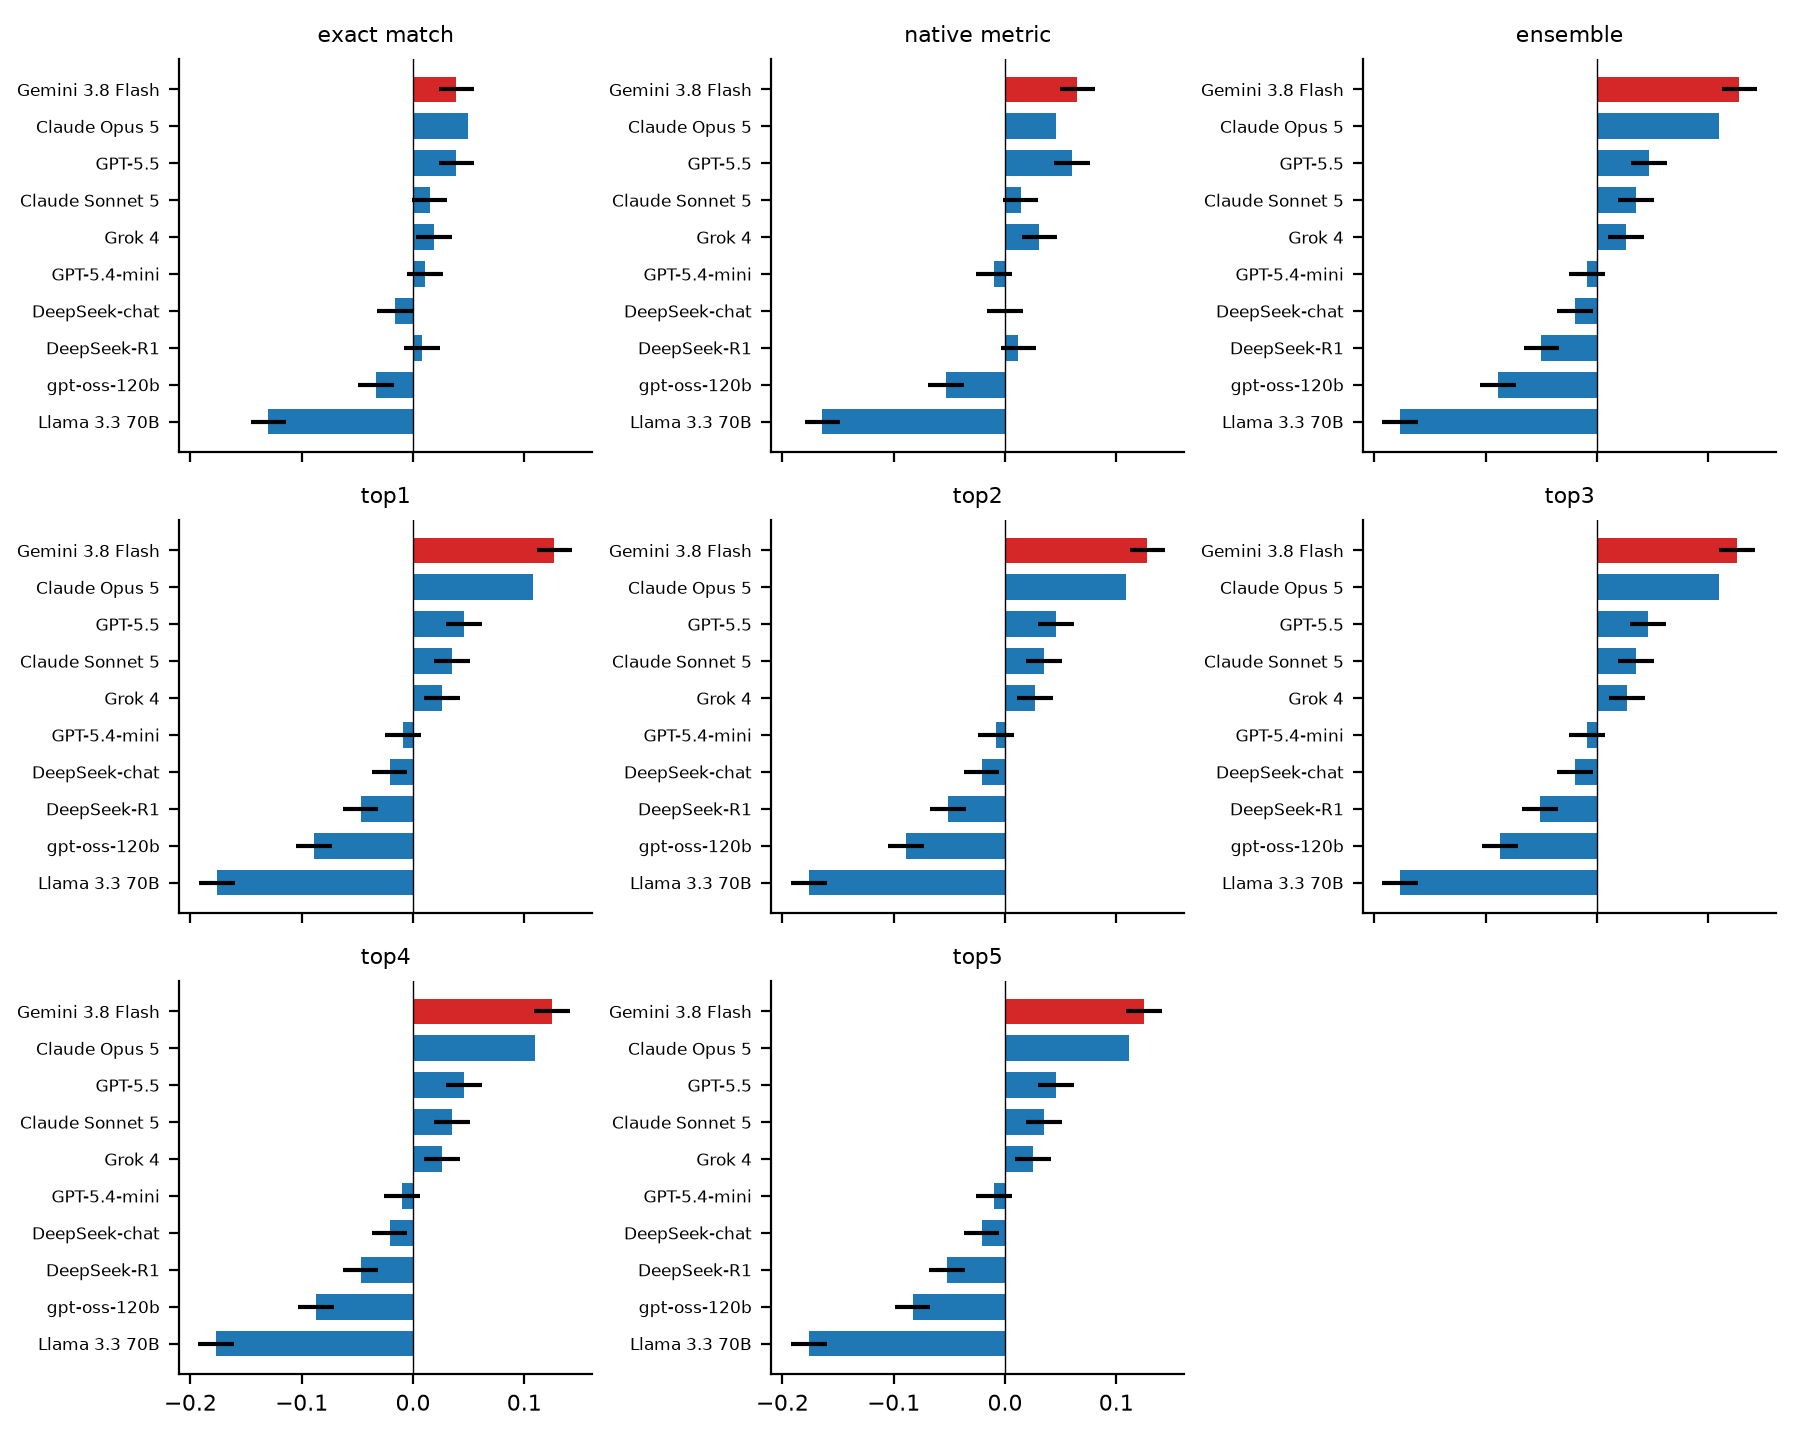
\includegraphics[width=0.9\textwidth]{fig_bt_all_rules.png}\caption{Bradley--Terry strengths ($\pm$ SE vs reference) under every reported rule; models fixed in the headline order.}\label{figall:fig_bt_all_rules}\end{figure}
\begin{figure}[htbp]\centering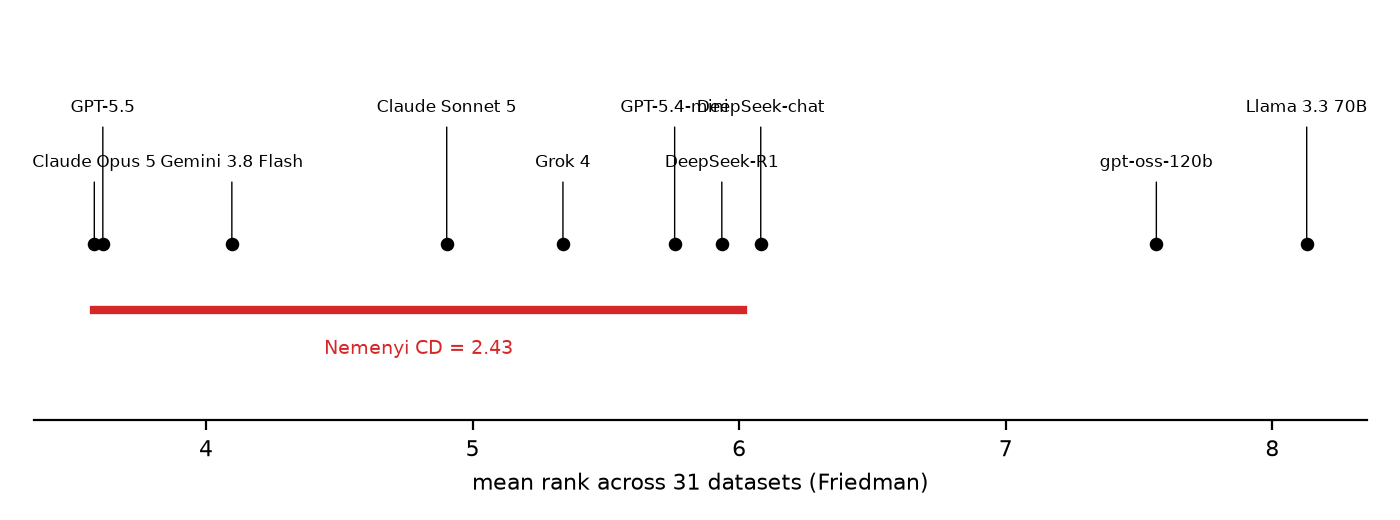
\includegraphics[width=0.9\textwidth]{fig_cd_diagram.png}\caption{Critical-difference view of the Friedman test under the headline rule: mean rank per model and the Nemenyi critical difference at $\alpha=.05$.}\label{figall:fig_cd_diagram}\end{figure}
\begin{figure}[htbp]\centering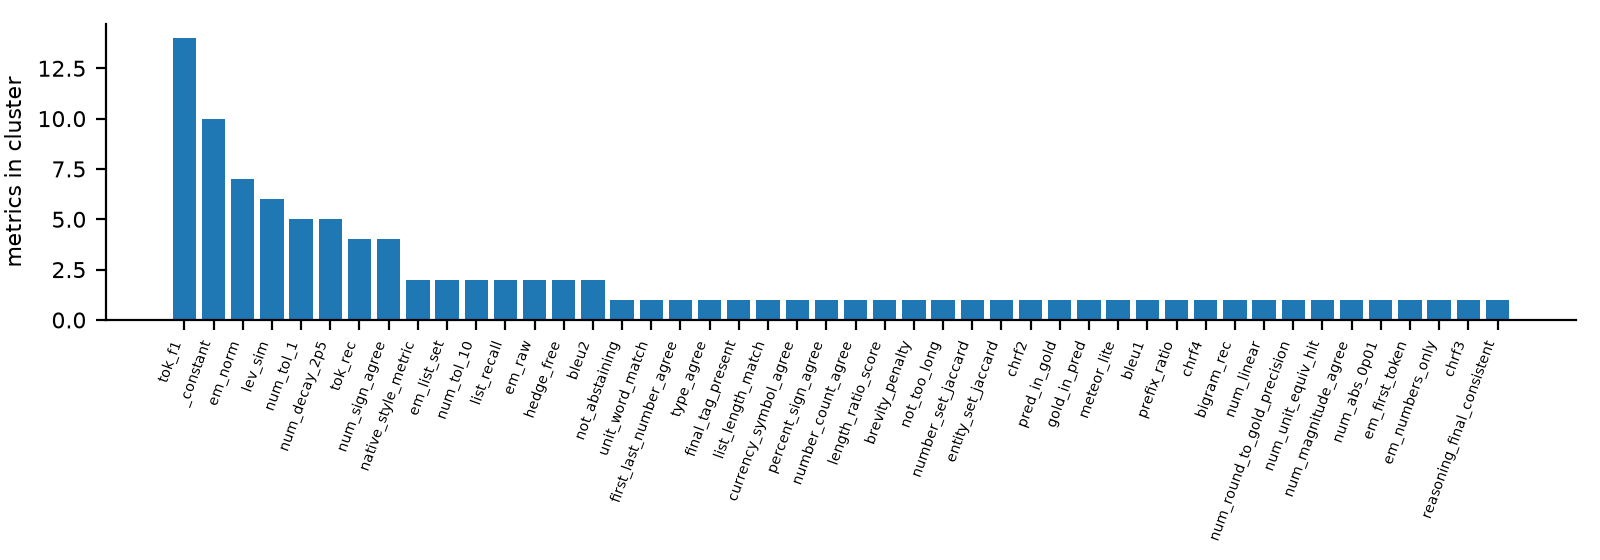
\includegraphics[width=0.9\textwidth]{fig_clusters.png}\caption{Cluster sizes after merging metrics with $|$Spearman$| \ge 0.95$ (45 representatives).}\label{figall:fig_clusters}\end{figure}
\begin{figure}[htbp]\centering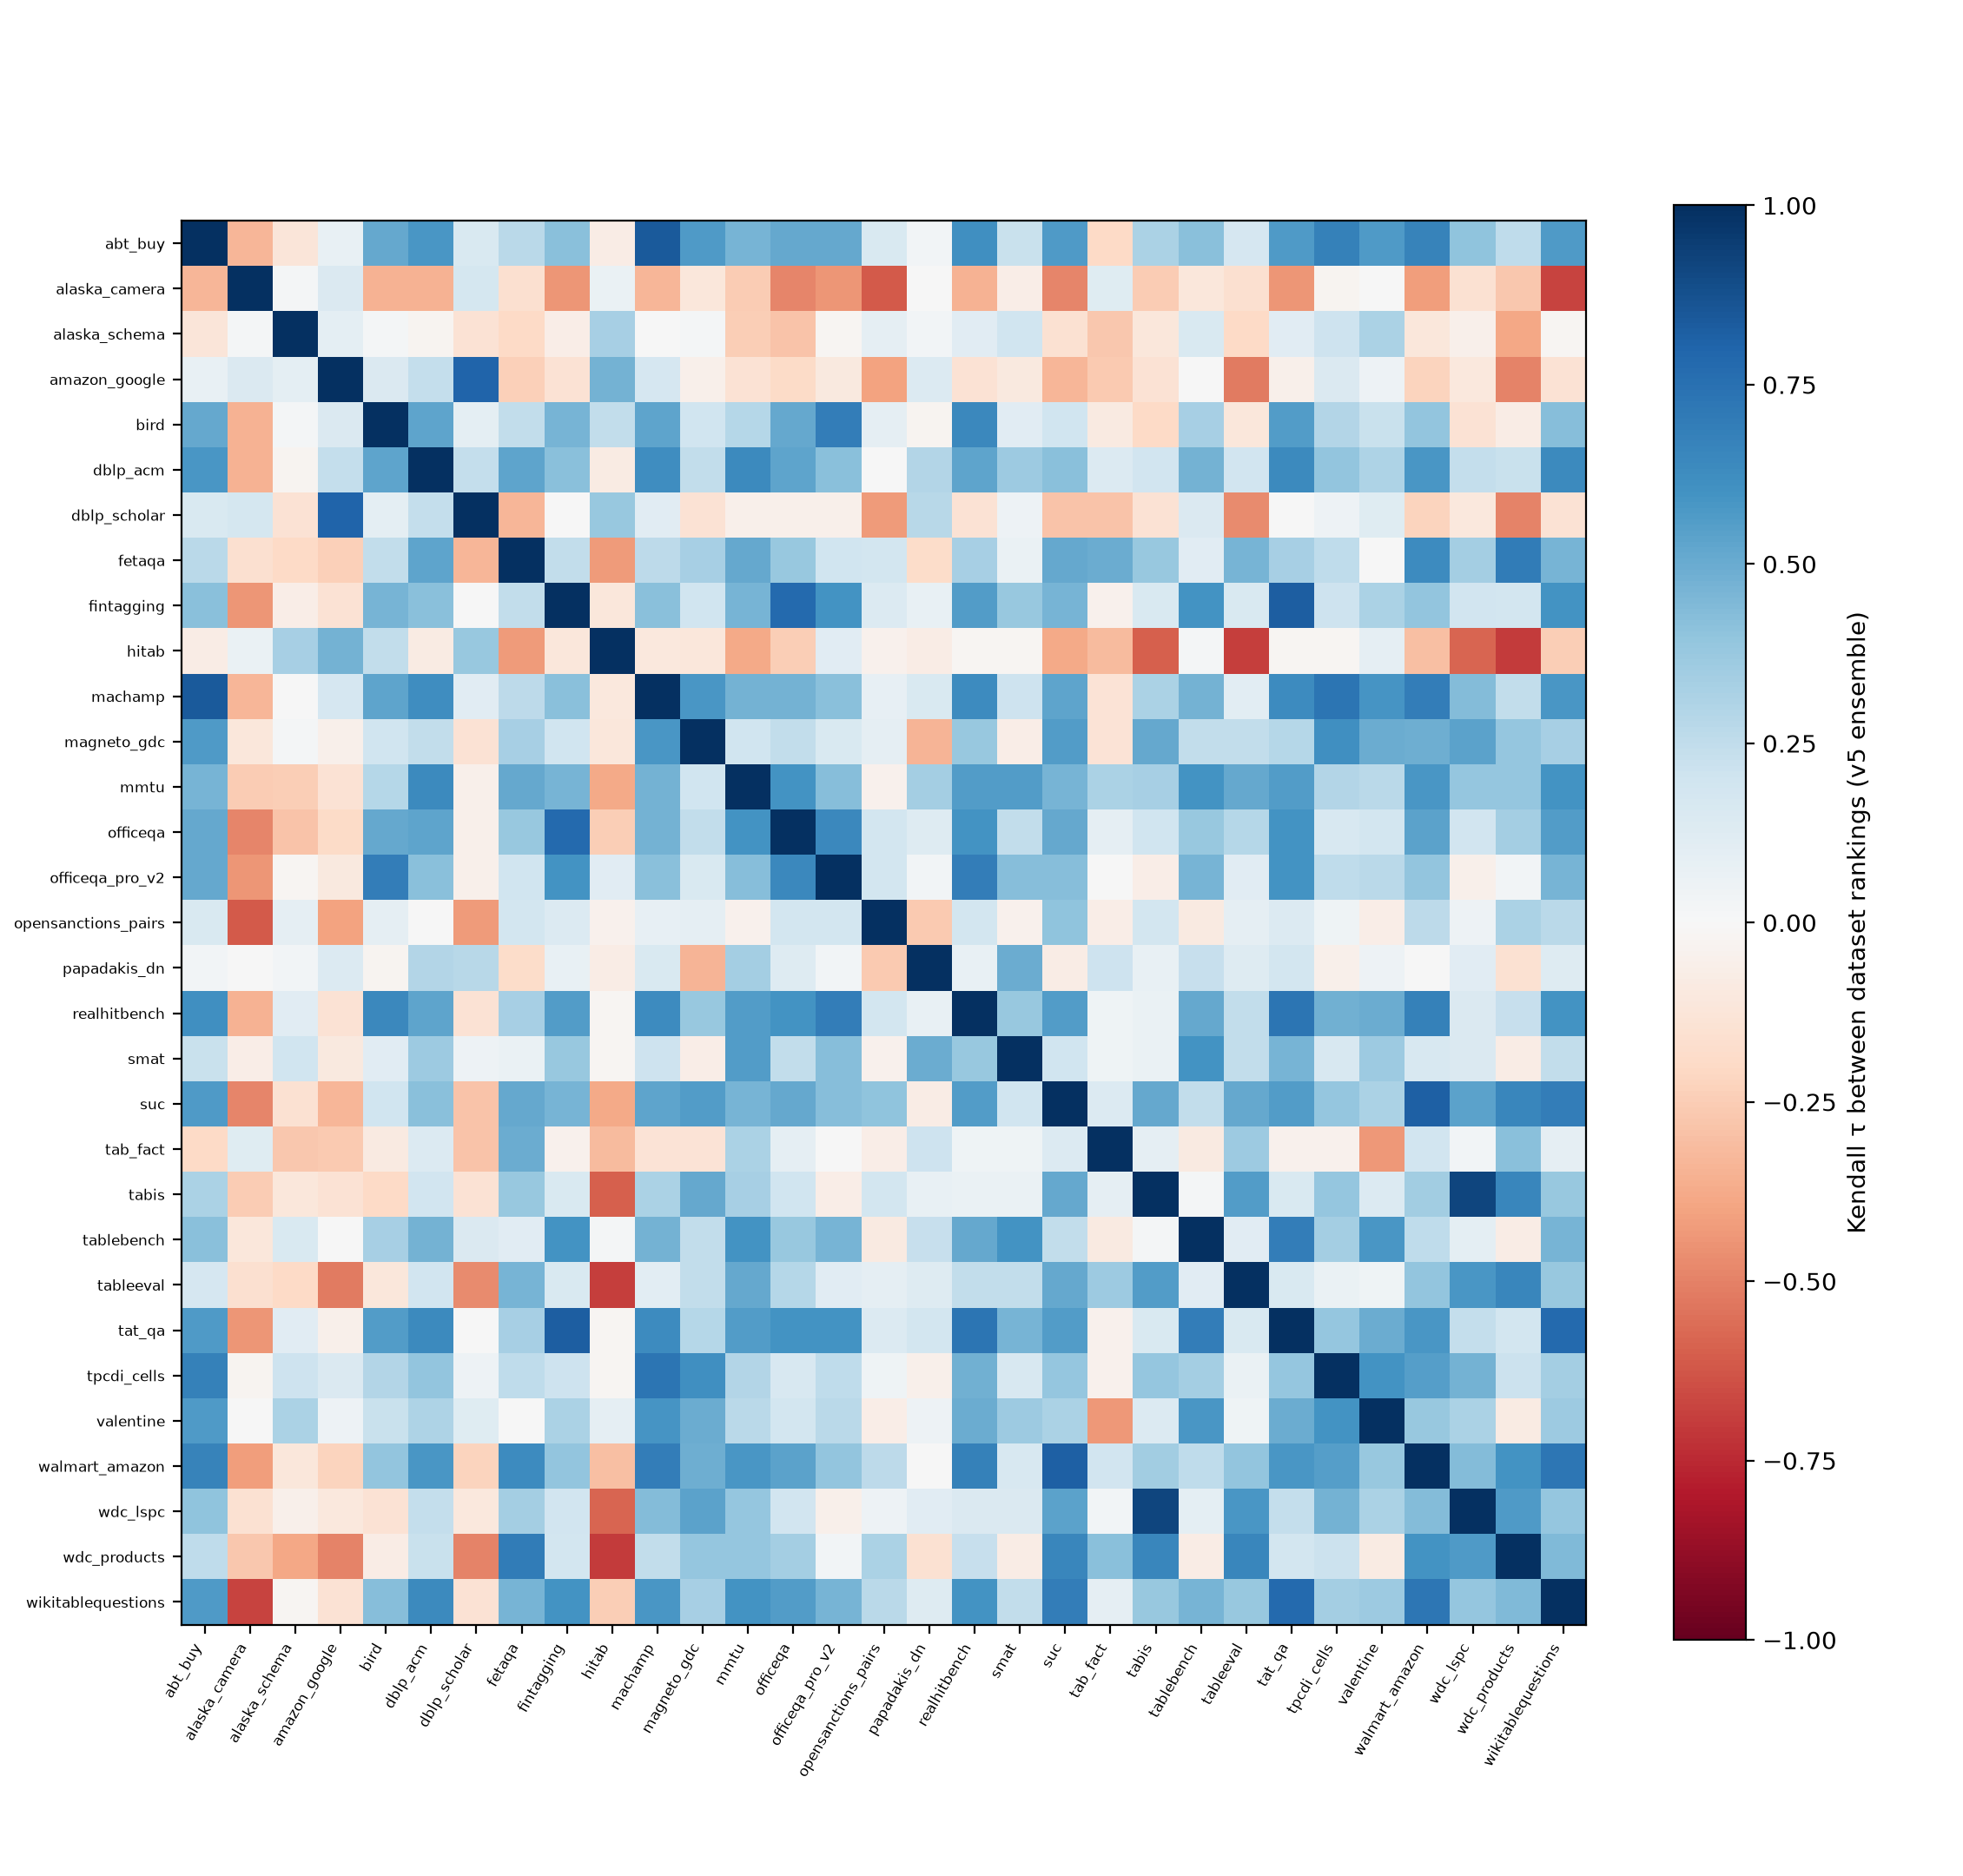
\includegraphics[width=0.9\textwidth]{fig_dataset_tau.png}\caption{Kendall $\tau$ between the model rankings of each pair of datasets under the headline rule.}\label{figall:fig_dataset_tau}\end{figure}
\begin{figure}[htbp]\centering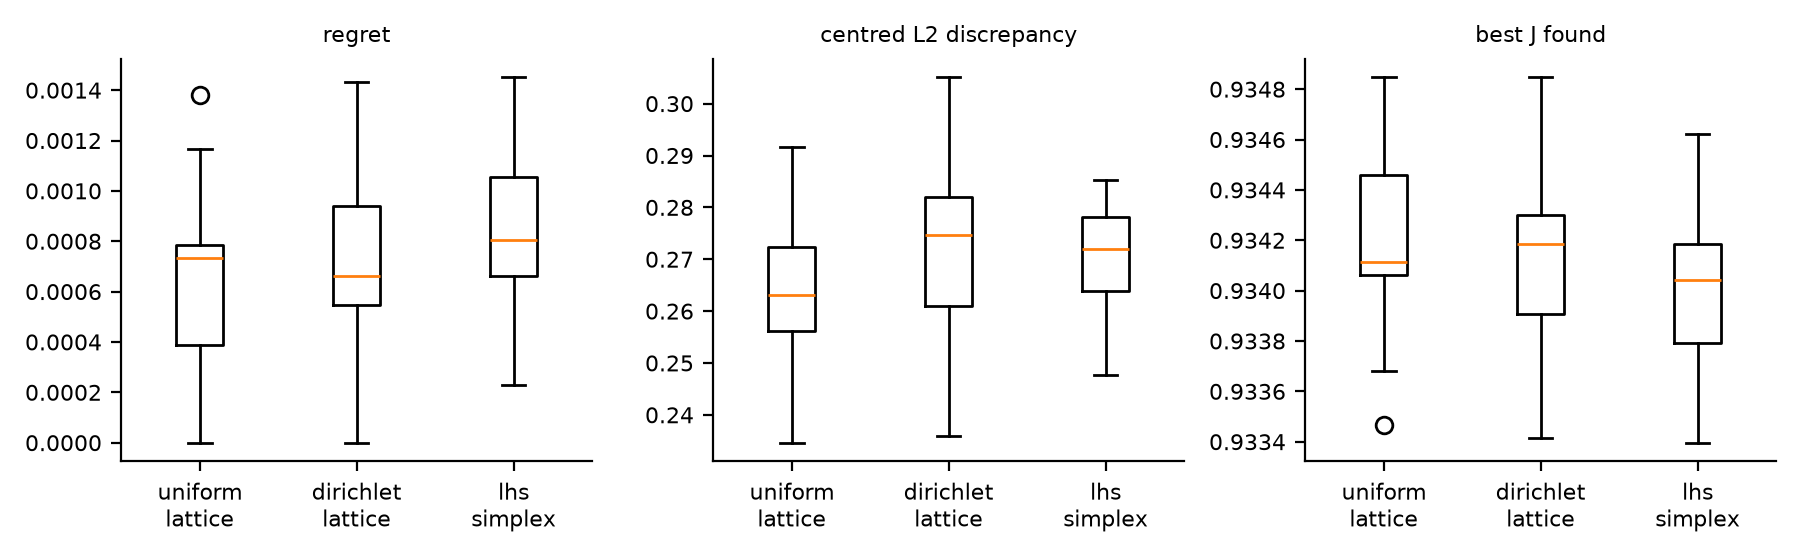
\includegraphics[width=0.9\textwidth]{fig_design_metrics.png}\caption{Sampled designs over 20 seeds against the exhaustive grid.}\label{figall:fig_design_metrics}\end{figure}
\begin{figure}[htbp]\centering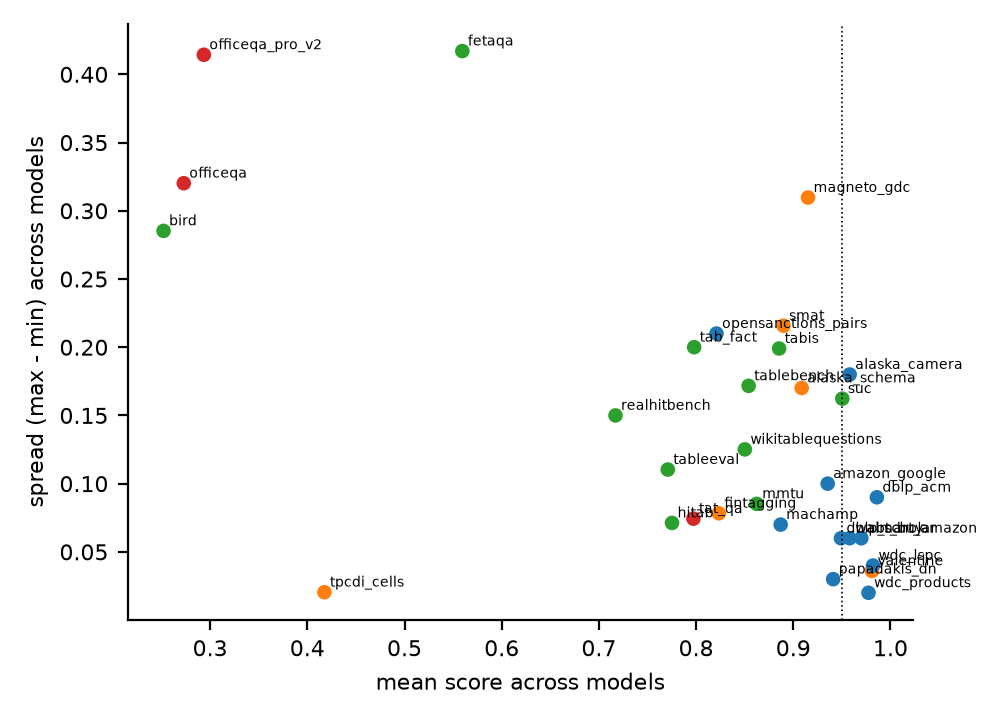
\includegraphics[width=0.9\textwidth]{fig_diagnostics_scatter.png}\caption{Dataset diagnostics: mean score against spread across models; dotted line marks the ceiling flag.}\label{figall:fig_diagnostics_scatter}\end{figure}
\begin{figure}[htbp]\centering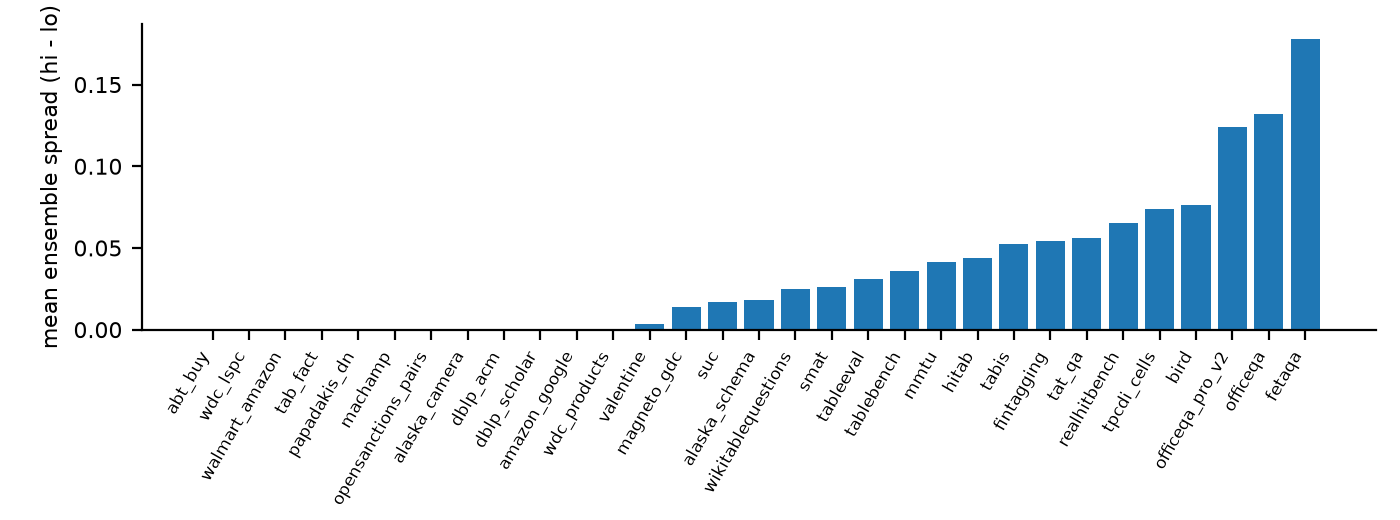
\includegraphics[width=0.9\textwidth]{fig_ensemble_spread.png}\caption{Ensemble uncertainty per dataset: mean spread of the per-answer score across the 100 weightings.}\label{figall:fig_ensemble_spread}\end{figure}
\begin{figure}[htbp]\centering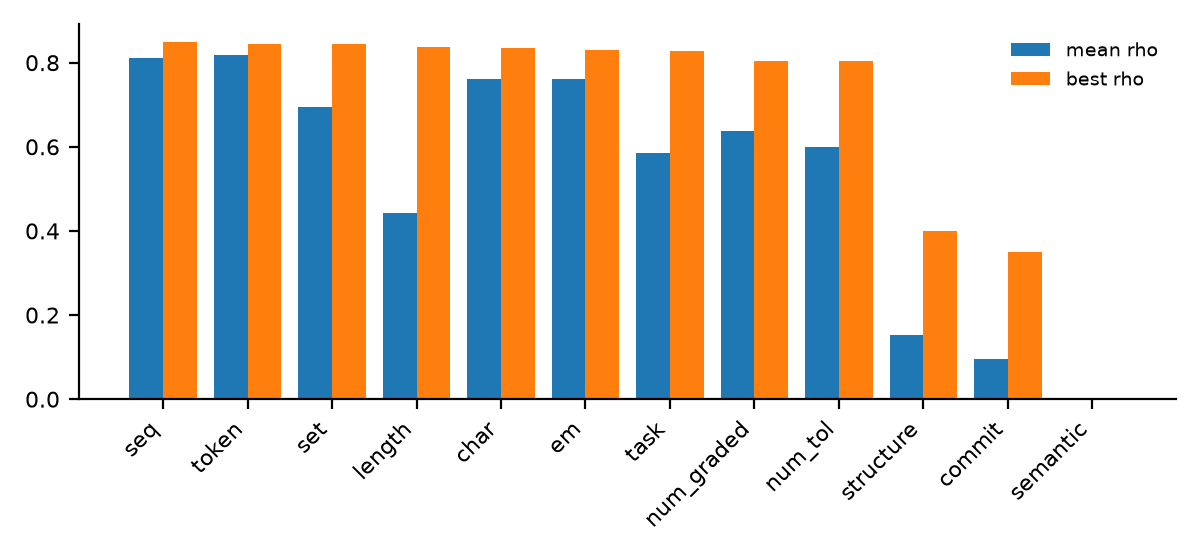
\includegraphics[width=0.9\textwidth]{fig_family_rho.png}\caption{Anchor $\rho$ per metric family: mean and best member.}\label{figall:fig_family_rho}\end{figure}
\begin{figure}[htbp]\centering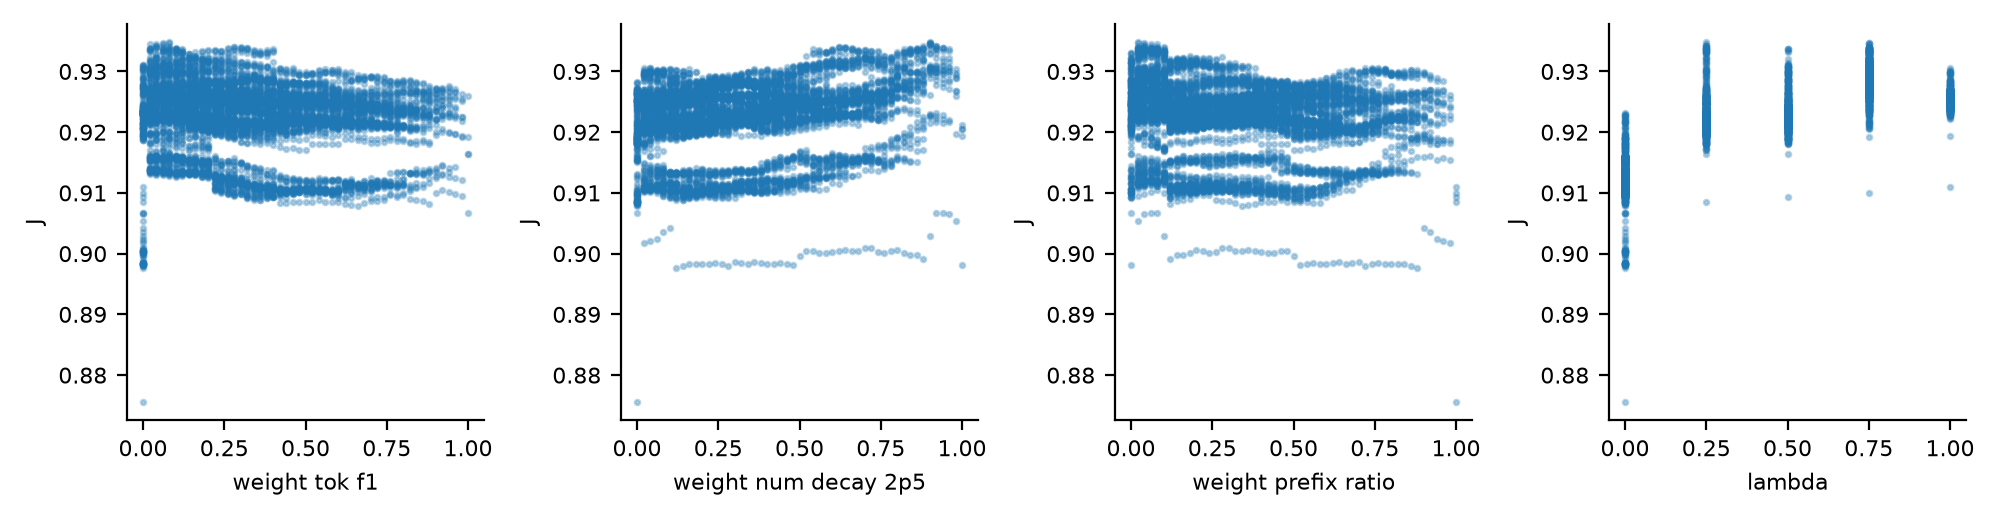
\includegraphics[width=0.9\textwidth]{fig_grid_marginals.png}\caption{Objective $J$ against each selected weight and the hedge penalty $\lambda$ over all 6,630 grid points.}\label{figall:fig_grid_marginals}\end{figure}
\begin{figure}[htbp]\centering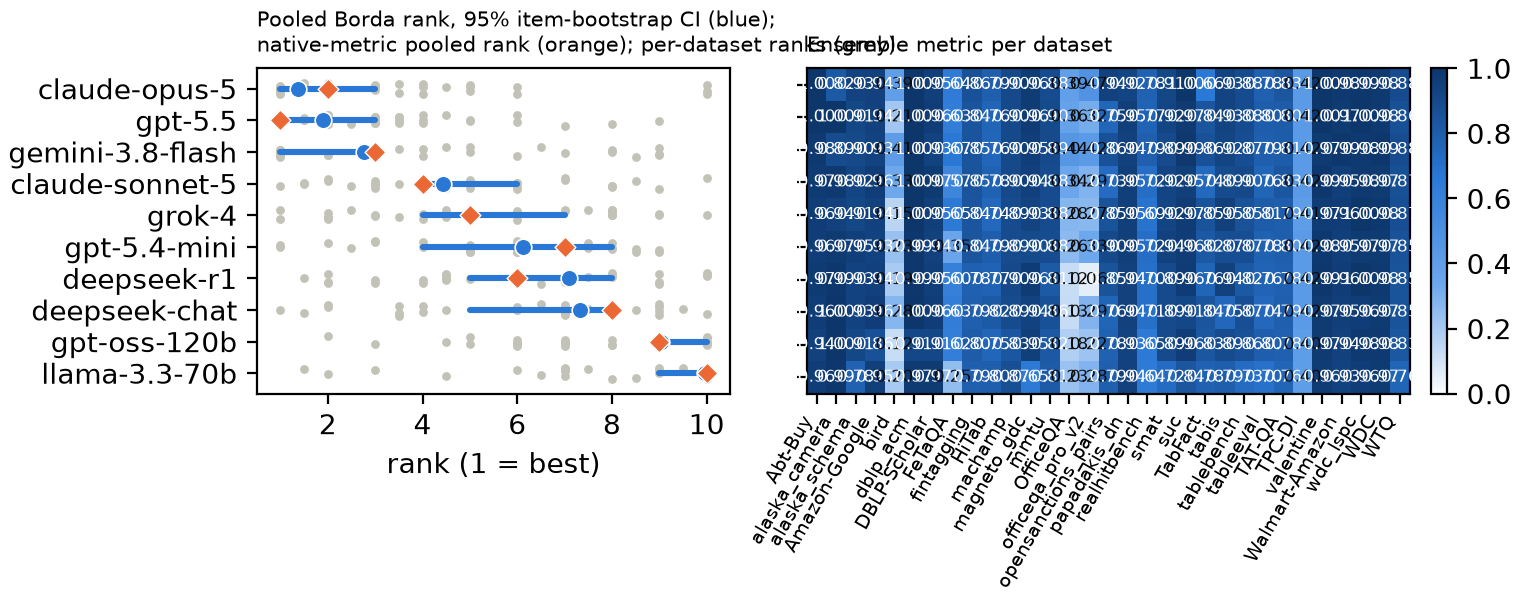
\includegraphics[width=0.9\textwidth]{fig_leaderboard.png}\caption{Ensemble leaderboard with bootstrap intervals and the native-metric ranking beside.}\label{figall:fig_leaderboard}\end{figure}
\begin{figure}[htbp]\centering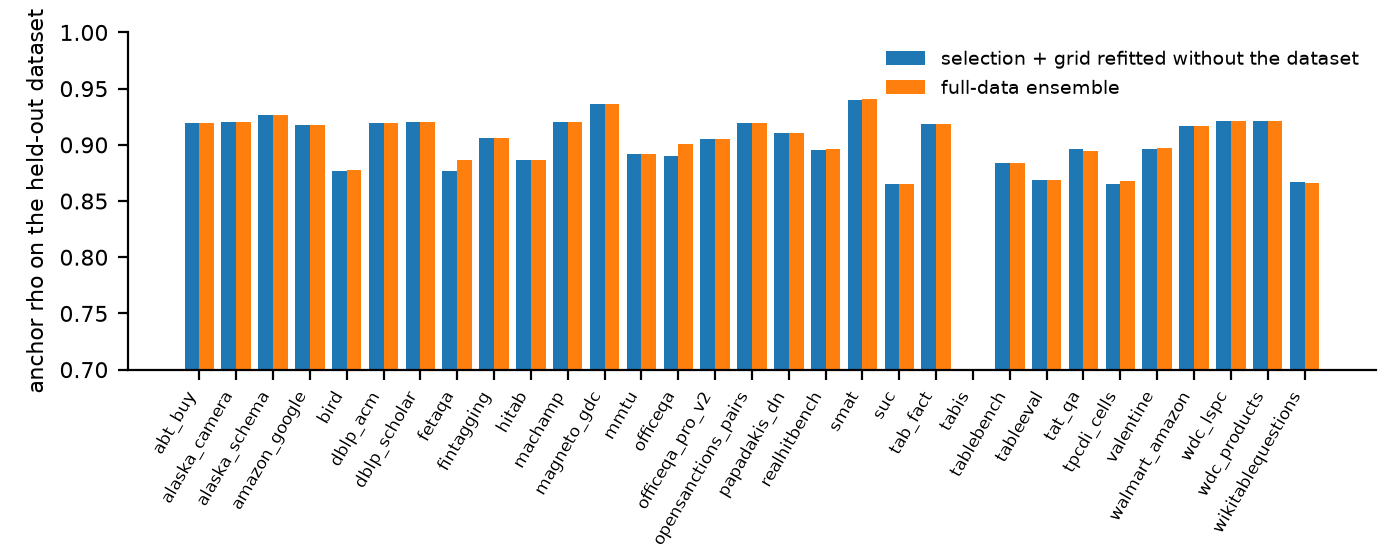
\includegraphics[width=0.9\textwidth]{fig_lodo.png}\caption{Leave-one-dataset-out: anchor $\rho$ on the held-out dataset under the re-fitted and the full-data ensemble.}\label{figall:fig_lodo}\end{figure}
\begin{figure}[htbp]\centering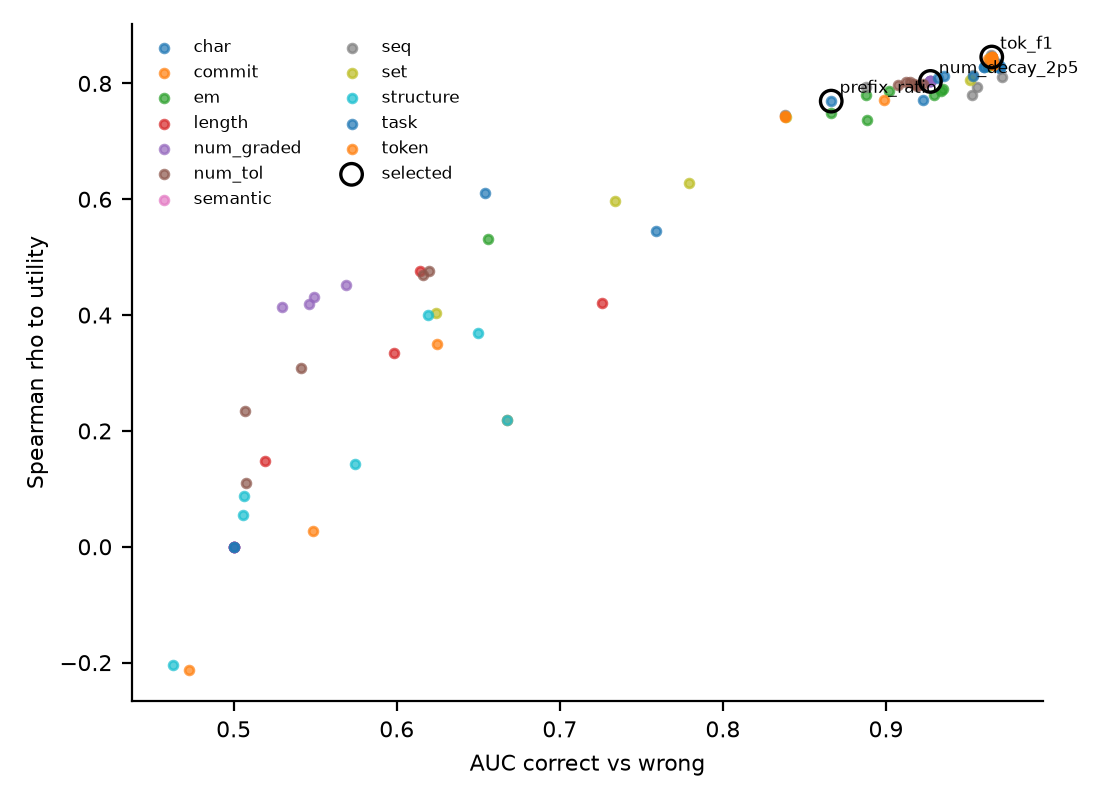
\includegraphics[width=0.9\textwidth]{fig_metric_library.png}\caption{The 100-metric library on the anchors: AUC against Spearman $\rho$, coloured by family; the three selected metrics are circled.}\label{figall:fig_metric_library}\end{figure}
\begin{figure}[htbp]\centering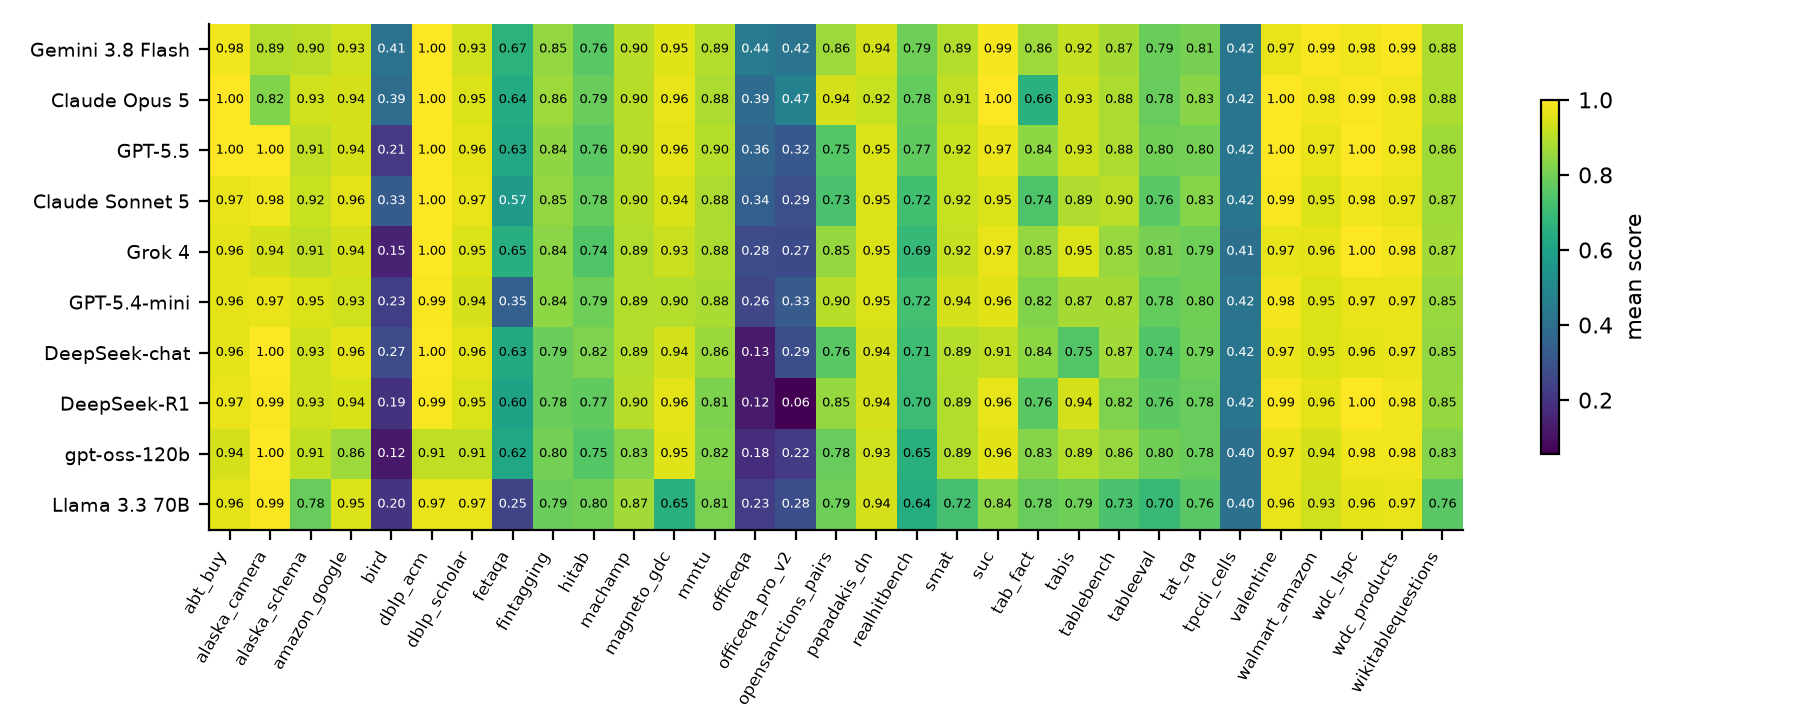
\includegraphics[width=0.9\textwidth]{fig_model_dataset_heatmap.png}\caption{Mean score per model and dataset under the headline rule.}\label{figall:fig_model_dataset_heatmap}\end{figure}
\begin{figure}[htbp]\centering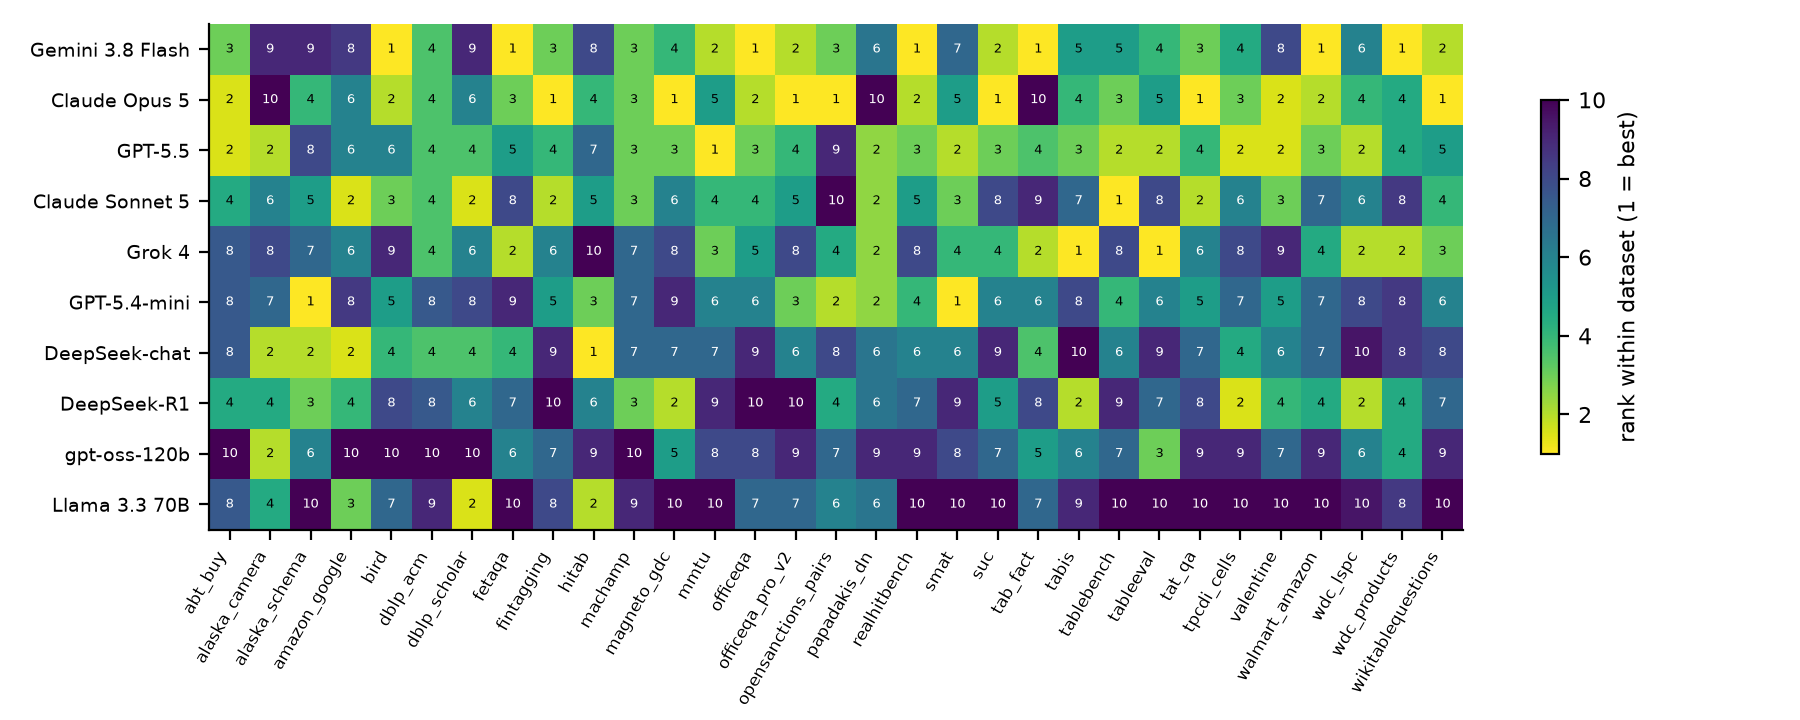
\includegraphics[width=0.9\textwidth]{fig_model_dataset_ranks.png}\caption{Rank per model and dataset under the headline rule.}\label{figall:fig_model_dataset_ranks}\end{figure}
\begin{figure}[htbp]\centering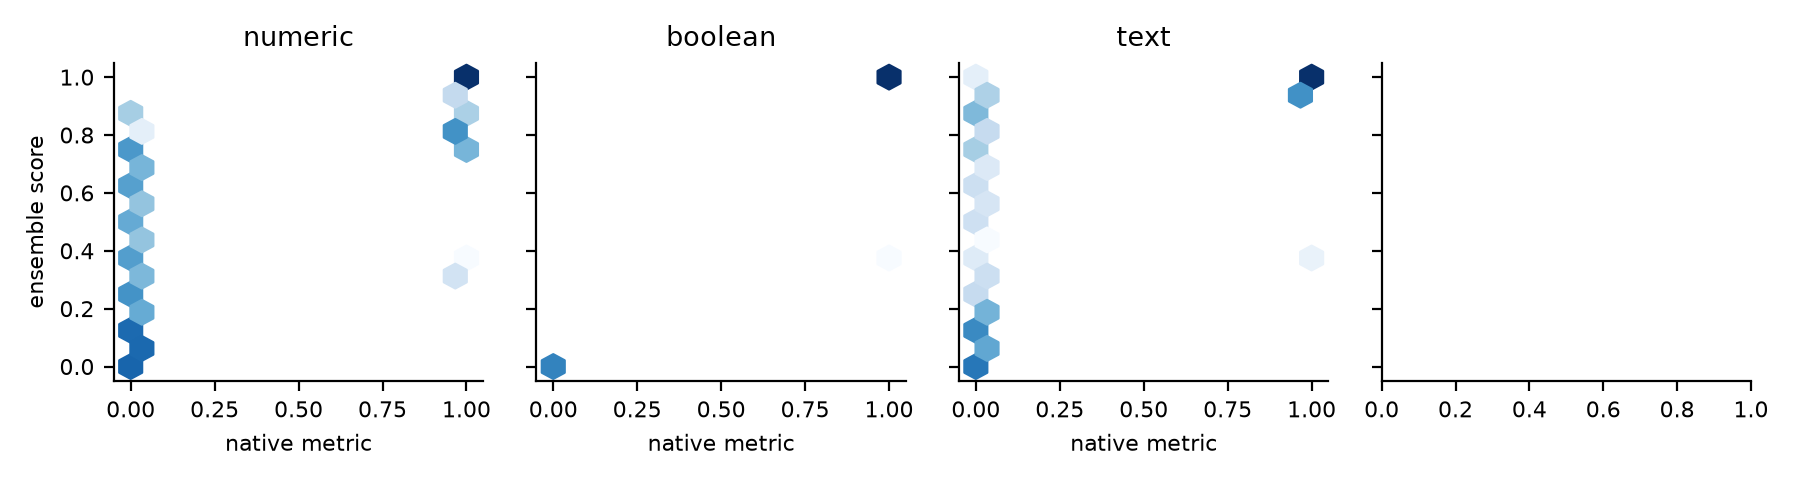
\includegraphics[width=0.9\textwidth]{fig_native_vs_ensemble.png}\caption{Per-answer native metric against the ensemble score, by answer type.}\label{figall:fig_native_vs_ensemble}\end{figure}
\begin{figure}[htbp]\centering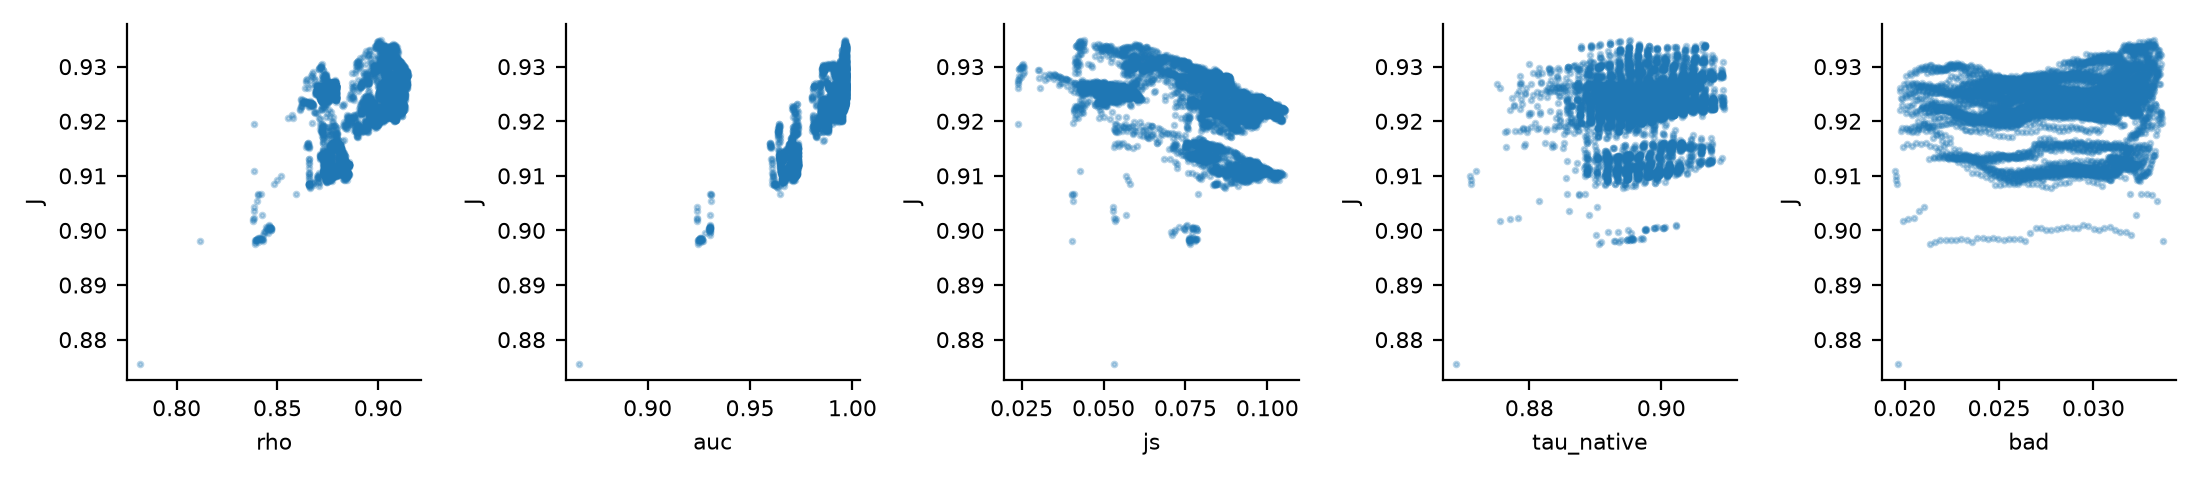
\includegraphics[width=0.9\textwidth]{fig_objective_terms.png}\caption{Objective $J$ against each of its five terms over the grid.}\label{figall:fig_objective_terms}\end{figure}
\begin{figure}[htbp]\centering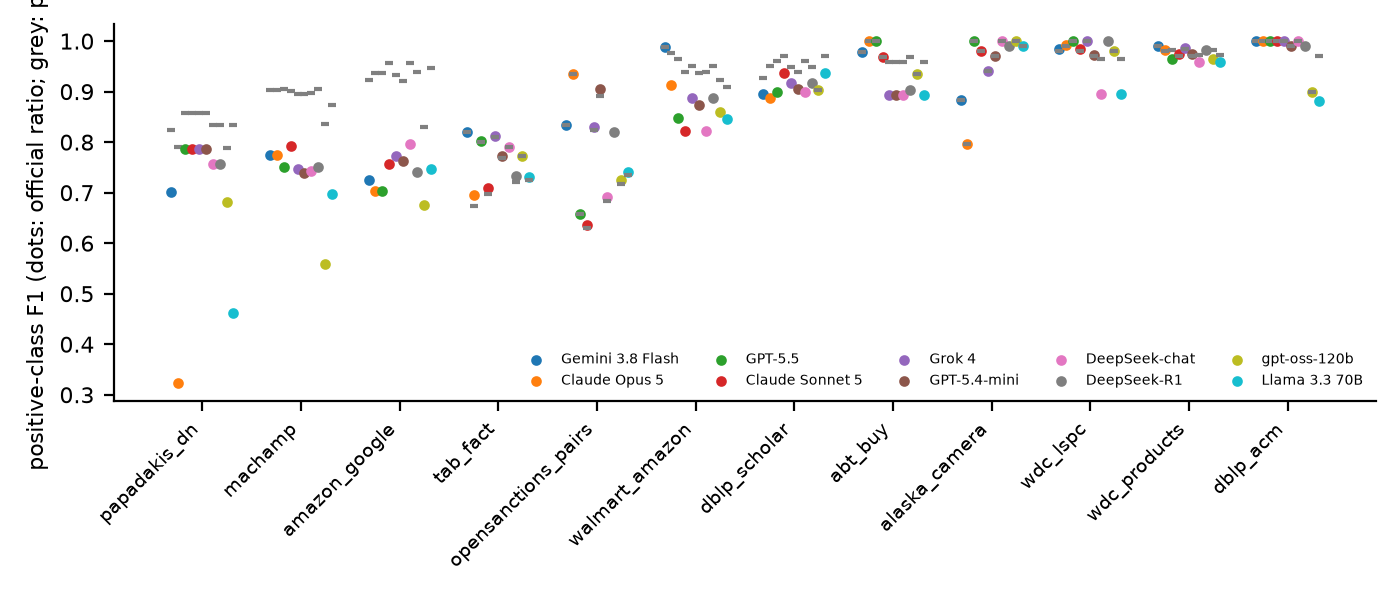
\includegraphics[width=0.9\textwidth]{fig_official_f1_models.png}\caption{Positive-class F1 on the balanced pool (grey) and at the official match ratio (coloured) per model and matching dataset.}\label{figall:fig_official_f1_models}\end{figure}
\begin{figure}[htbp]\centering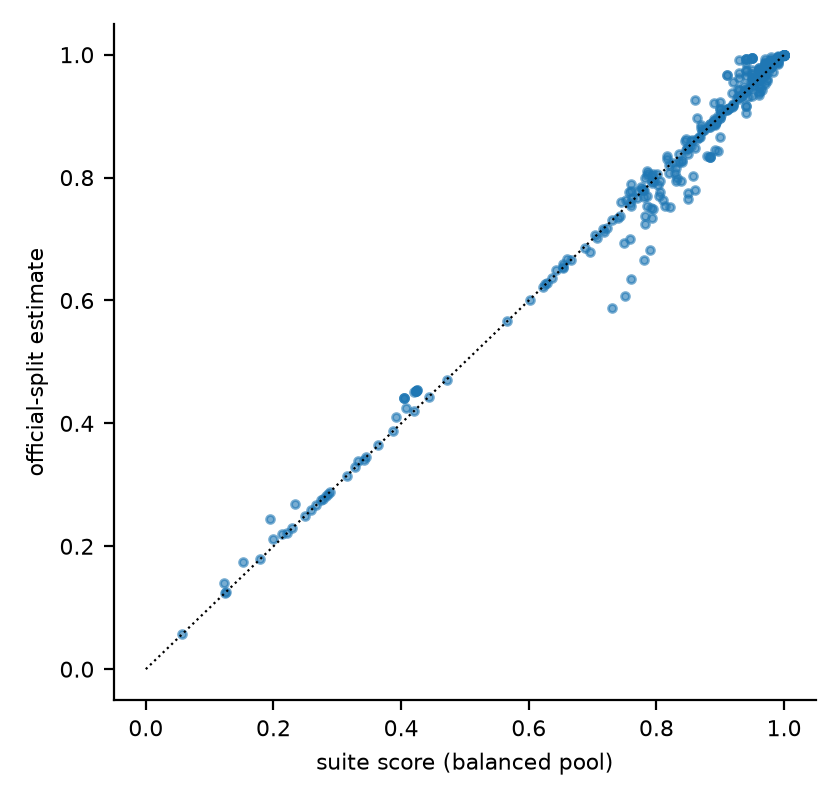
\includegraphics[width=0.9\textwidth]{fig_official_scatter.png}\caption{Suite score against post-stratified official-split estimate for every (dataset, model) pair under the headline rule.}\label{figall:fig_official_scatter}\end{figure}
\begin{figure}[htbp]\centering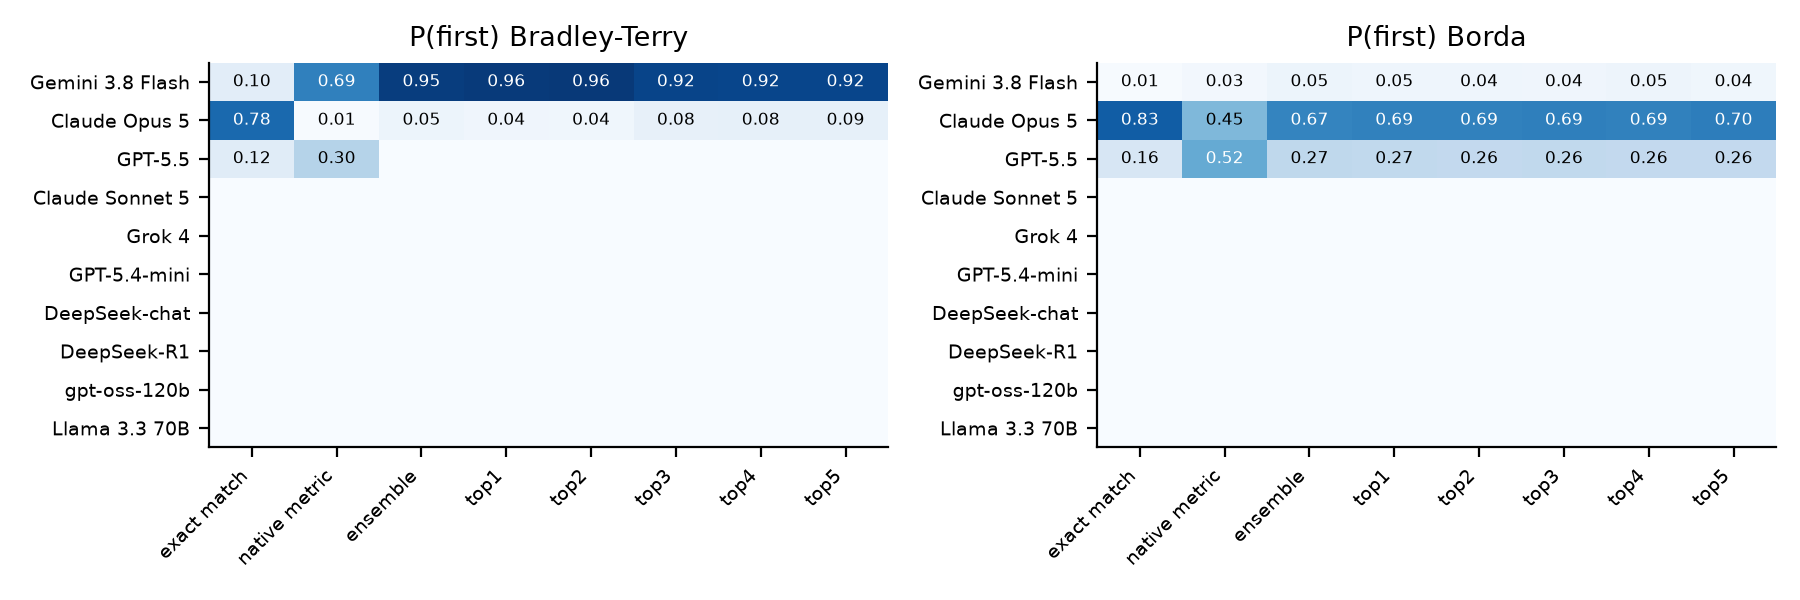
\includegraphics[width=0.9\textwidth]{fig_p_first.png}\caption{Bootstrap probability of first place under every rule, by pooling method.}\label{figall:fig_p_first}\end{figure}
\begin{figure}[htbp]\centering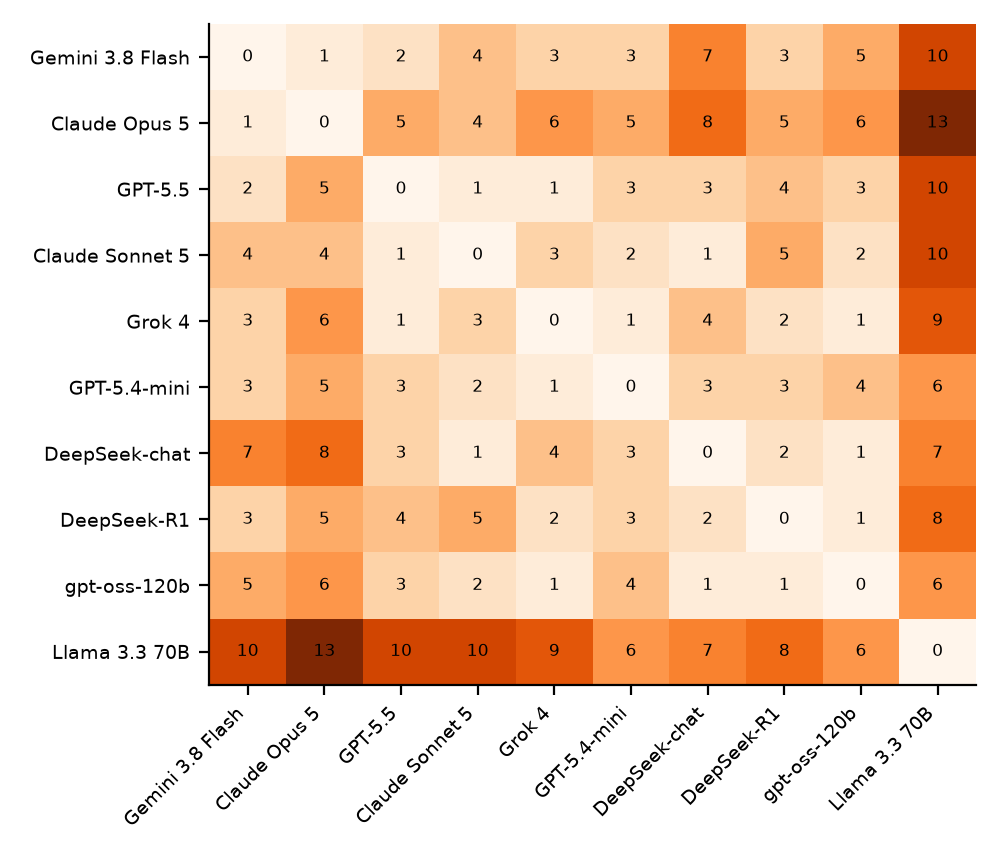
\includegraphics[width=0.9\textwidth]{fig_pairwise_significance.png}\caption{Number of datasets (of 31) in which the per-item paired test separates each pair of models under the headline rule (Holm within dataset).}\label{figall:fig_pairwise_significance}\end{figure}
\begin{figure}[htbp]\centering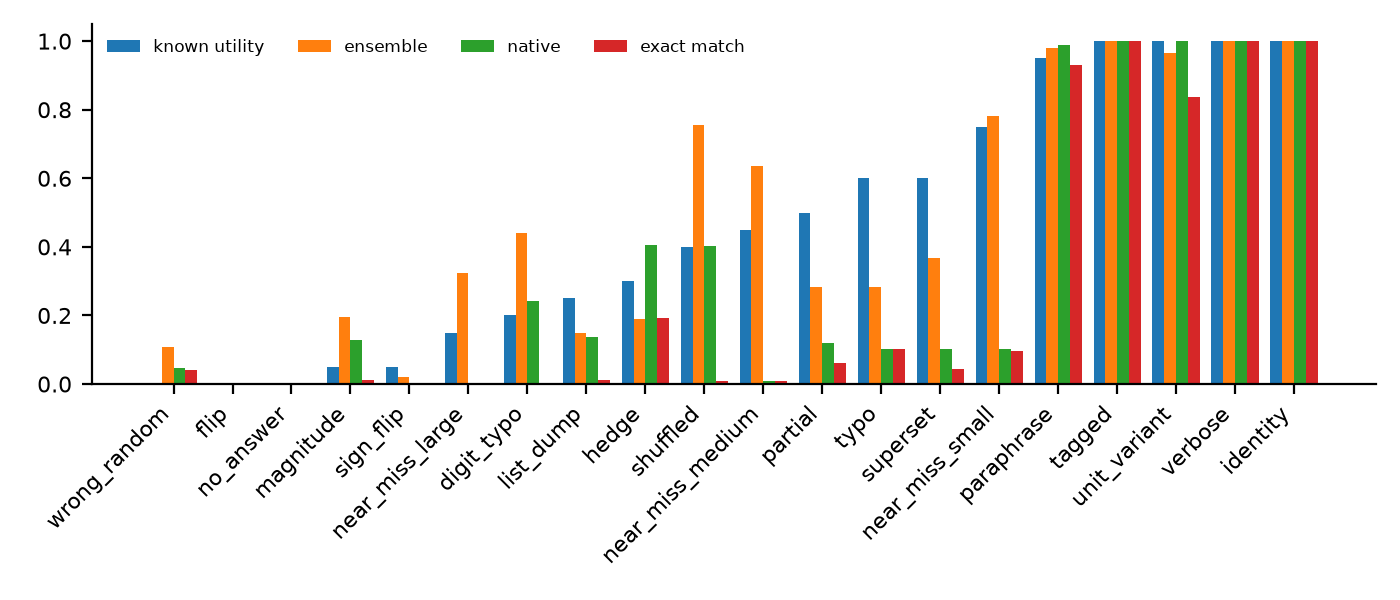
\includegraphics[width=0.9\textwidth]{fig_probe_operators.png}\caption{Mean score per anchor operator under the ensemble, the native metric and exact match, against known utility.}\label{figall:fig_probe_operators}\end{figure}
\begin{figure}[htbp]\centering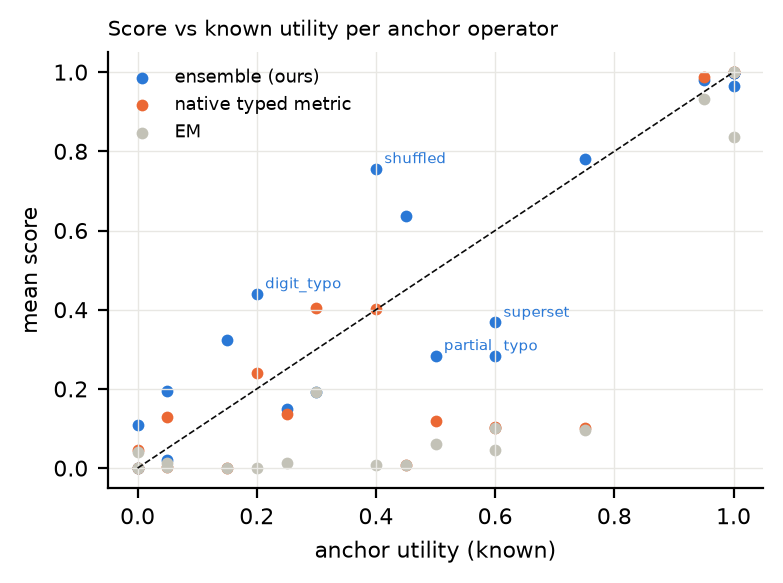
\includegraphics[width=0.9\textwidth]{fig_probes.png}\caption{Probes: mean score per anchor operator against known utility for the ensemble and the single-metric baselines.}\label{figall:fig_probes}\end{figure}
\begin{figure}[htbp]\centering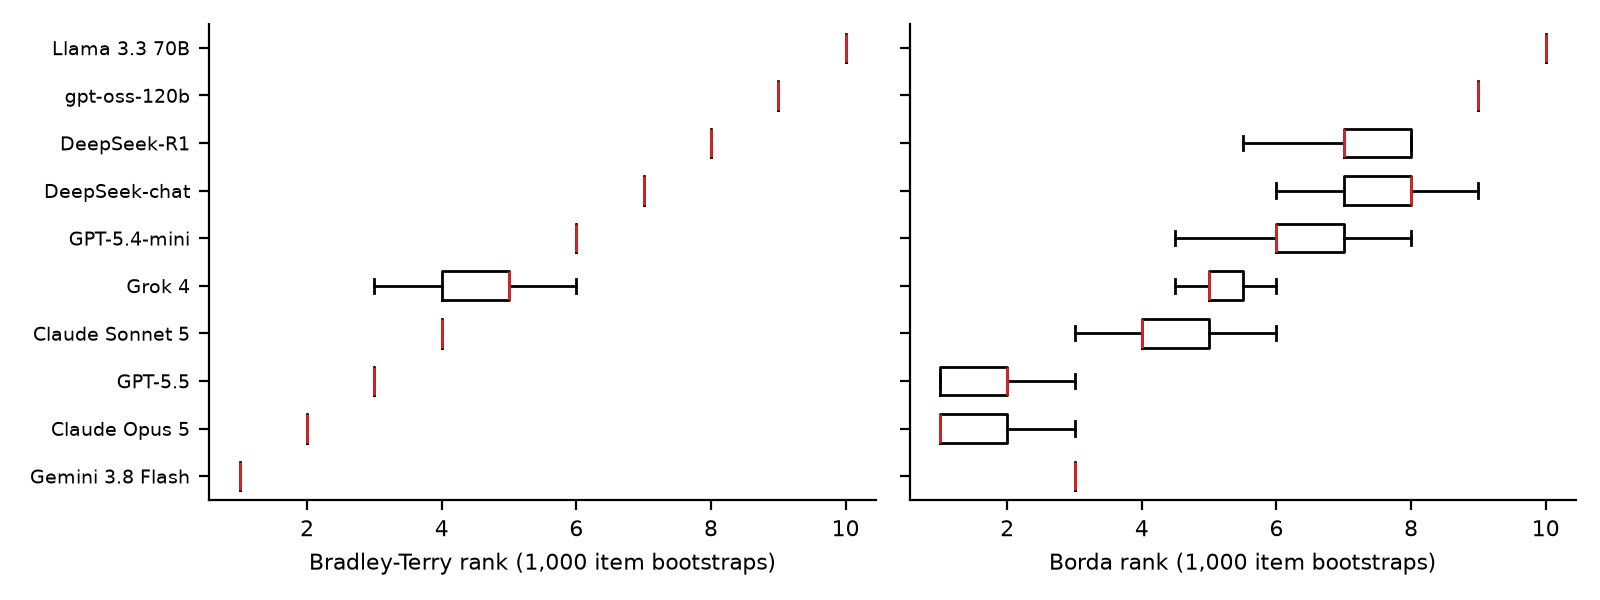
\includegraphics[width=0.9\textwidth]{fig_rank_bootstrap.png}\caption{Bootstrap distribution of each model's rank under the headline rule (ensemble).}\label{figall:fig_rank_bootstrap}\end{figure}
\begin{figure}[htbp]\centering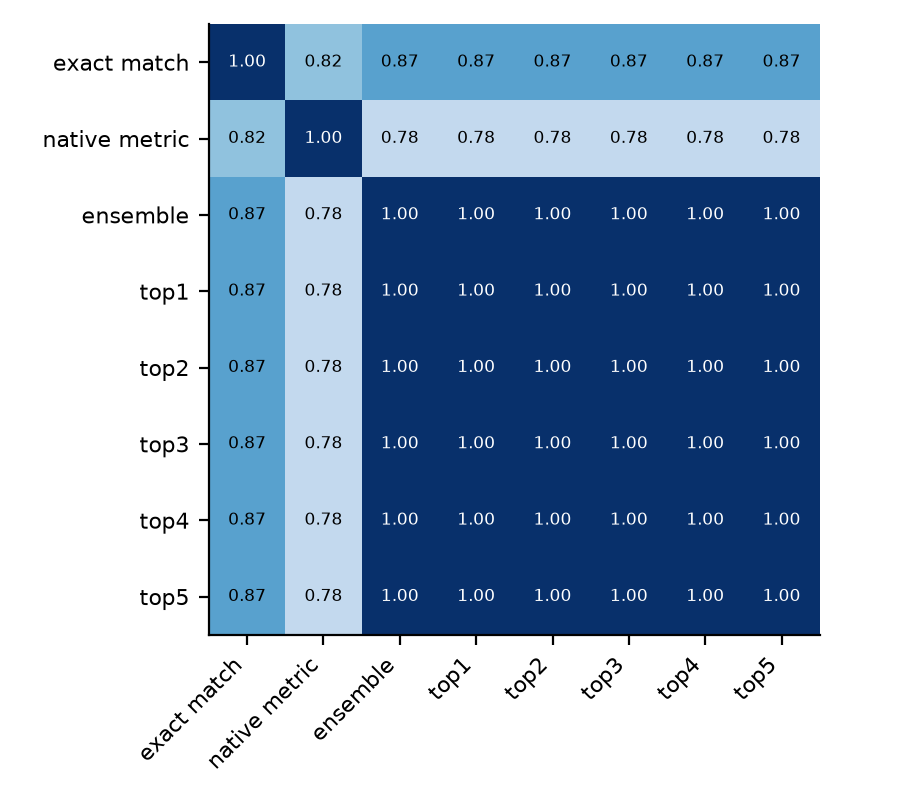
\includegraphics[width=0.9\textwidth]{fig_rule_agreement.png}\caption{Kendall $\tau$ between the Bradley--Terry rankings of each pair of rules.}\label{figall:fig_rule_agreement}\end{figure}
\begin{figure}[htbp]\centering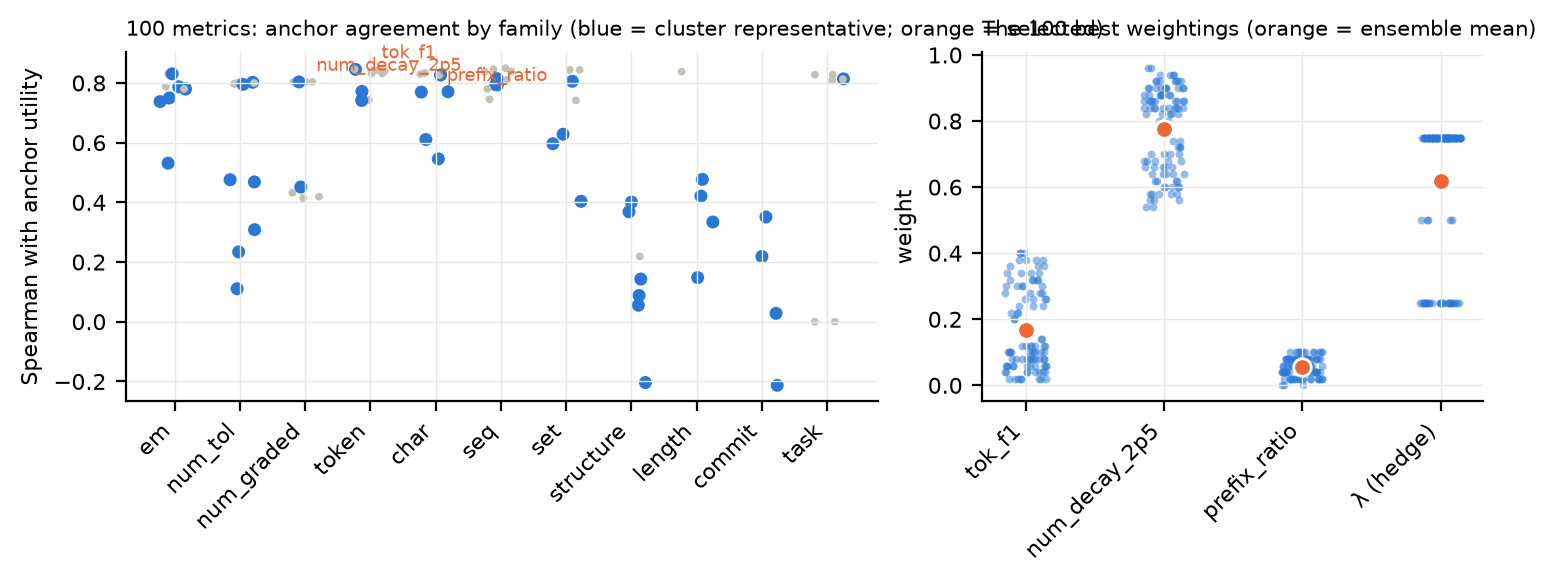
\includegraphics[width=0.9\textwidth]{fig_selection.png}\caption{Metric selection: anchor agreement of every library metric with the selected set marked.}\label{figall:fig_selection}\end{figure}
\begin{figure}[htbp]\centering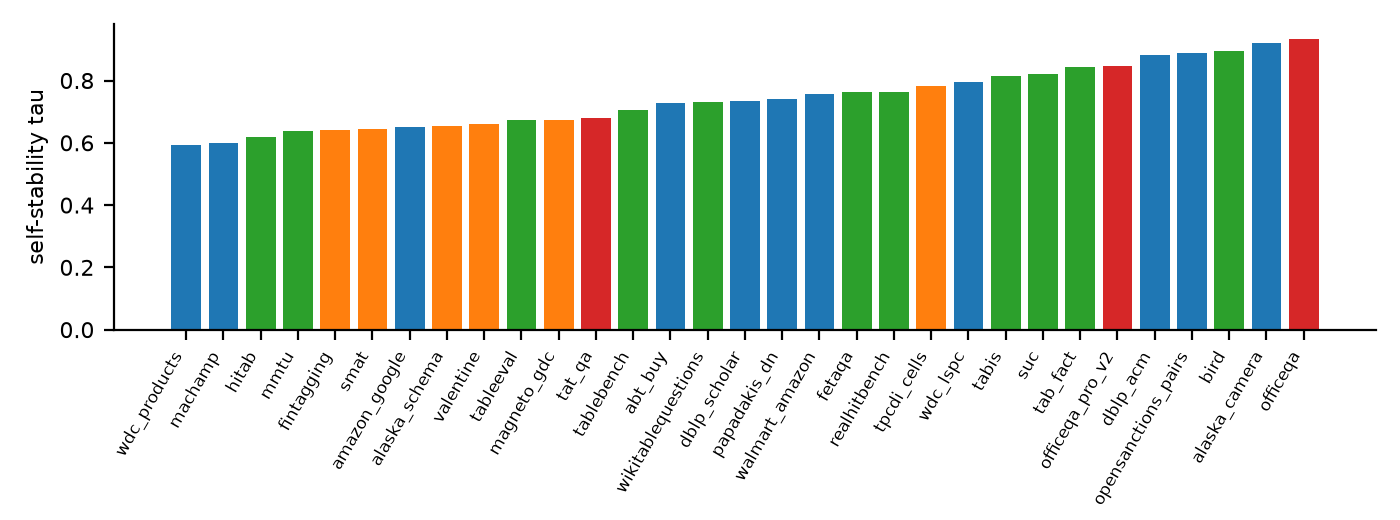
\includegraphics[width=0.9\textwidth]{fig_self_stability.png}\caption{Self-stability of each dataset's model ranking (Kendall $\tau$ between bootstrap halves).}\label{figall:fig_self_stability}\end{figure}
\begin{figure}[htbp]\centering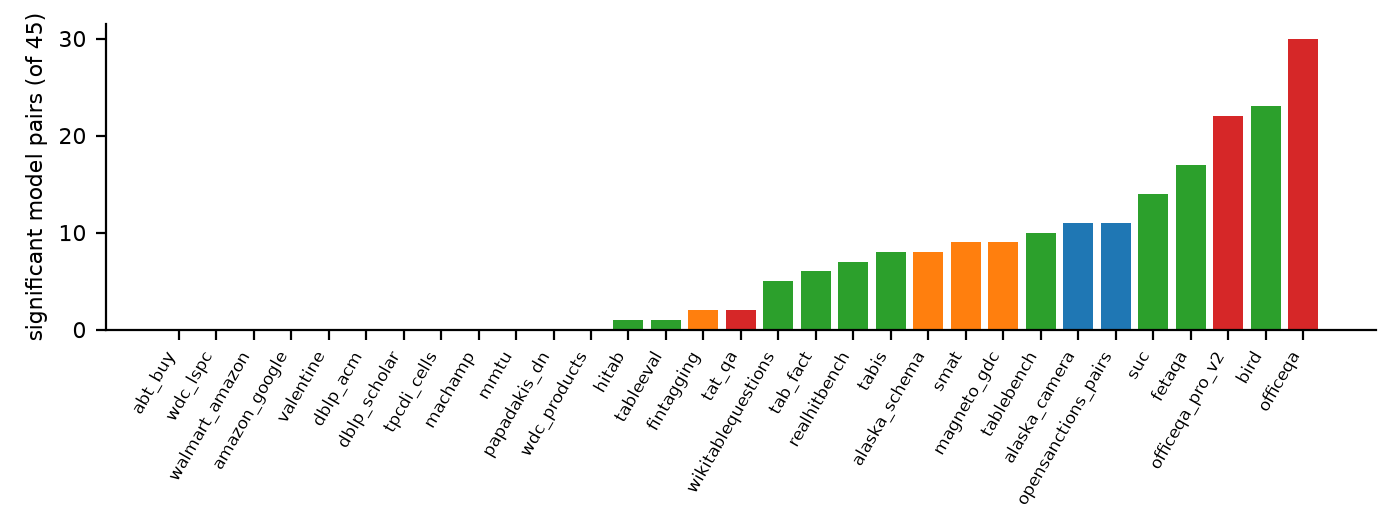
\includegraphics[width=0.9\textwidth]{fig_significant_pairs_per_dataset.png}\caption{How many of the 45 model pairs each dataset separates at the item level under the headline rule (colour = family).}\label{figall:fig_significant_pairs_per_dataset}\end{figure}
\begin{figure}[htbp]\centering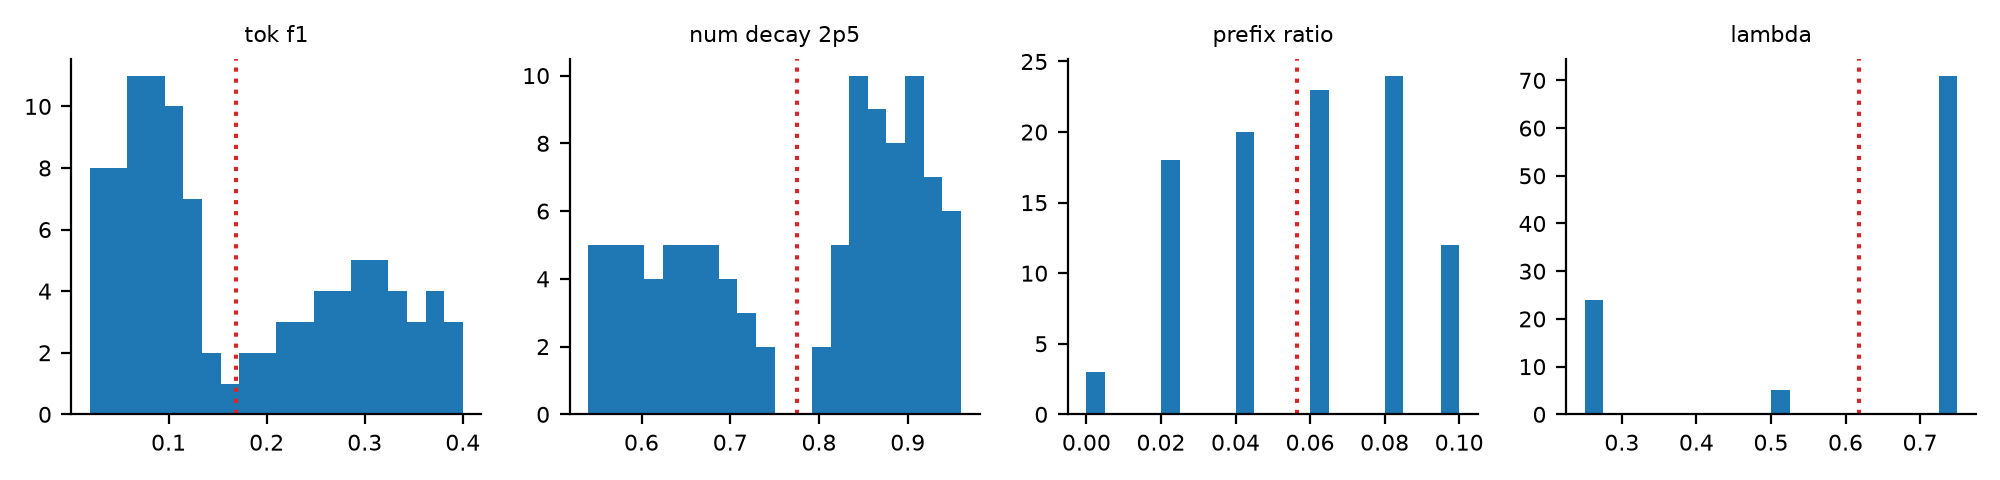
\includegraphics[width=0.9\textwidth]{fig_top100_weights.png}\caption{Weights and $\lambda$ of the 100 best grid points that form the ensemble (dotted = mean).}\label{figall:fig_top100_weights}\end{figure}
\clearpage
\section{All tables}
Every saved table, one file each under \texttt{tables/}; include any in the main text with \texttt{\textbackslash input}.
\begin{table}[htbp]
\centering\tiny
\caption{Baselines under the same objective.}
\label{tab:baselines}
\setlength{\tabcolsep}{3pt}
\begin{tabular}{p{0.572\linewidth}rrrrrr}
\toprule
baseline & rho & auc & js & bad & tau\_\allowbreak{}native & J \\
\midrule
native\_\allowbreak{}style\_\allowbreak{}metric & 0.826 & 0.935 & 0.031 & 0.014 & 0.992 & 0.925 \\
em\_\allowbreak{}norm & 0.849 & 0.963 & 0.024 & 0.012 & 0.924 & 0.928 \\
tok\_\allowbreak{}f1 & 0.859 & 0.965 & 0.079 & 0.032 & 0.888 & 0.907 \\
rouge\_\allowbreak{}l & 0.862 & 0.965 & 0.082 & 0.032 & 0.892 & 0.907 \\
num\_\allowbreak{}tol\_\allowbreak{}1 & 0.806 & 0.919 & 0.032 & 0.016 & 0.946 & 0.909 \\
uniform\_\allowbreak{}over\_\allowbreak{}selected\_\allowbreak{}no\_\allowbreak{}gate & 0.882 & 0.970 & 0.098 & 0.028 & 0.900 & 0.911 \\
ensemble\_\allowbreak{}top100 & 0.904 & 0.996 & 0.053 & 0.032 & 0.898 & 0.934 \\
\bottomrule
\end{tabular}
\end{table}

\clearpage
\begin{table}[htbp]
\centering\tiny
\caption{Sampled designs vs the exhaustive grid (best $J$ = 0.9348 over 6630 points).}
\label{tab:designs_summary}
\setlength{\tabcolsep}{3pt}
\begin{tabular}{p{0.185\linewidth}p{0.120\linewidth}rp{0.120\linewidth}rp{0.163\linewidth}p{0.120\linewidth}r}
\toprule
design & best\_\allowbreak{}J\_\allowbreak{}mean & best\_\allowbreak{}J\_\allowbreak{}sd & regret\_\allowbreak{}mean & regret\_\allowbreak{}max & min\_\allowbreak{}pairwise\_\allowbreak{}L1 & discrepancy & zero\_\allowbreak{}share \\
\midrule
dirichlet\_\allowbreak{}lattice & 0.9342 & 0.0004 & 0.0007 & 0.0014 & 0.0400 & 0.2728 & 0.0615 \\
lhs\_\allowbreak{}simplex & 0.9340 & 0.0003 & 0.0008 & 0.0015 & 0.0400 & 0.2702 & 0.0555 \\
uniform\_\allowbreak{}lattice & 0.9342 & 0.0003 & 0.0007 & 0.0014 & 0.0400 & 0.2639 & 0.1115 \\
\bottomrule
\end{tabular}
\end{table}

\clearpage
\begin{landscape}
\tiny
\setlength{\tabcolsep}{3pt}
\begin{longtable}{p{0.147\linewidth}p{0.073\linewidth}p{0.073\linewidth}p{0.073\linewidth}p{0.073\linewidth}p{0.073\linewidth}p{0.073\linewidth}p{0.073\linewidth}p{0.073\linewidth}p{0.073\linewidth}p{0.073\linewidth}}
\caption{Dataset diagnostics under the headline rule.}\label{tab:diagnostics}\\
\toprule
dataset & family & mean\_\allowbreak{}score & spread\_\allowbreak{}across\_\allowbreak{}models & floor & ceiling & share\_\allowbreak{}constant\_\allowbreak{}bootstrap\_\allowbreak{}rankings & ranking\_\allowbreak{}self\_\allowbreak{}stability\_\allowbreak{}tau & tau\_\allowbreak{}to\_\allowbreak{}others\_\allowbreak{}mean & n\_\allowbreak{}items & exclude\_\allowbreak{}from\_\allowbreak{}objective \\
\midrule
abt\_\allowbreak{}buy & EM & 0.970 & 0.060 & no & no & 0.000 & 0.726 & 0.346 & 100 & no \\
alaska\_\allowbreak{}camera & EM & 0.958 & 0.180 & no & no & 0.000 & 0.919 & -0.226 & 100 & no \\
alaska\_\allowbreak{}schema & SM & 0.909 & 0.170 & no & no & 0.000 & 0.653 & -0.024 & 93 & no \\
amazon\_\allowbreak{}google & EM & 0.935 & 0.100 & no & no & 0.000 & 0.650 & -0.043 & 100 & no \\
bird & TQA & 0.252 & 0.285 & no & no & 0.000 & 0.894 & 0.225 & 100 & no \\
dblp\_\allowbreak{}acm & EM & 0.986 & 0.090 & no & no & 0.000 & 0.884 & 0.337 & 100 & no \\
dblp\_\allowbreak{}scholar & EM & 0.949 & 0.060 & no & no & 0.000 & 0.733 & -0.030 & 100 & no \\
fetaqa & TQA & 0.559 & 0.417 & no & no & 0.000 & 0.764 & 0.223 & 100 & no \\
fintagging & SM & 0.823 & 0.078 & no & no & 0.000 & 0.641 & 0.281 & 100 & no \\
hitab & TQA & 0.775 & 0.071 & no & no & 0.000 & 0.618 & -0.128 & 100 & no \\
machamp & EM & 0.887 & 0.070 & no & no & 0.000 & 0.600 & 0.358 & 100 & no \\
magneto\_\allowbreak{}gdc & SM & 0.915 & 0.310 & no & no & 0.000 & 0.675 & 0.232 & 100 & no \\
mmtu & TQA & 0.862 & 0.085 & no & no & 0.000 & 0.639 & 0.324 & 100 & no \\
officeqa & FIN & 0.273 & 0.320 & no & no & 0.000 & 0.935 & 0.286 & 100 & no \\
officeqa\_\allowbreak{}pro\_\allowbreak{}v2 & FIN & 0.294 & 0.414 & no & no & 0.000 & 0.847 & 0.259 & 90 & no \\
opensanctions\_\allowbreak{}pairs & EM & 0.821 & 0.210 & no & no & 0.000 & 0.888 & 0.034 & 100 & no \\
papadakis\_\allowbreak{}dn & EM & 0.941 & 0.030 & no & no & 0.002 & 0.739 & 0.067 & 100 & no \\
realhitbench & TQA & 0.717 & 0.150 & no & no & 0.000 & 0.764 & 0.347 & 100 & no \\
smat & SM & 0.890 & 0.216 & no & no & 0.000 & 0.643 & 0.200 & 100 & no \\
suc & TQA & 0.950 & 0.162 & no & no & 0.000 & 0.820 & 0.314 & 100 & no \\
tab\_\allowbreak{}fact & TQA & 0.798 & 0.200 & no & no & 0.000 & 0.845 & 0.012 & 100 & no \\
tabis & TQA & 0.885 & 0.199 & no & no & 0.000 & 0.814 & 0.181 & 100 & no \\
tablebench & TQA & 0.854 & 0.172 & no & no & 0.000 & 0.705 & 0.273 & 100 & no \\
tableeval & TQA & 0.771 & 0.110 & no & no & 0.000 & 0.674 & 0.154 & 100 & no \\
tat\_\allowbreak{}qa & FIN & 0.797 & 0.074 & no & no & 0.000 & 0.678 & 0.363 & 100 & no \\
tpcdi\_\allowbreak{}cells & SM & 0.418 & 0.020 & no & no & 0.000 & 0.783 & 0.285 & 100 & no \\
valentine & SM & 0.981 & 0.036 & no & yes & 0.000 & 0.661 & 0.245 & 100 & yes \\
walmart\_\allowbreak{}amazon & EM & 0.958 & 0.060 & no & no & 0.000 & 0.755 & 0.348 & 100 & no \\
wdc\_\allowbreak{}lspc & EM & 0.982 & 0.040 & no & yes & 0.004 & 0.796 & 0.218 & 100 & yes \\
wdc\_\allowbreak{}products & EM & 0.977 & 0.020 & no & yes & 0.006 & 0.592 & 0.162 & 100 & yes \\
wikitablequestions & TQA & 0.850 & 0.125 & no & no & 0.000 & 0.732 & 0.342 & 100 & no \\
\bottomrule
\end{longtable}
\normalsize
\end{landscape}

\clearpage
\scriptsize
\setlength{\tabcolsep}{3pt}
\begin{longtable}{p{0.110\linewidth}p{0.832\linewidth}}
\caption{Ensemble summary.}\label{tab:ensemble}\\
\toprule
quantity & value \\
\midrule
selected & ["tok\_\allowbreak{}f1", "num\_\allowbreak{}decay\_\allowbreak{}2p5", "prefix\_\allowbreak{}ratio"] \\
selected\_\allowbreak{}idx & [33, 24, 51] \\
hedge\_\allowbreak{}col & 89 \\
alpha & {"rho": 0.3, "auc": 0.15, "consistency": 0.2, "native": 0.15, "bad": 0.2} \\
grid\_\allowbreak{}step & 0.020 \\
n\_\allowbreak{}grid & 6630 \\
top\_\allowbreak{}k & 100 \\
mean\_\allowbreak{}weights & {"tok\_\allowbreak{}f1": 0.16860000000000006, "num\_\allowbreak{}decay\_\allowbreak{}2p5": 0.7748, "prefix\_\allowbreak{}ratio": 0.05659999999999999} \\
mean\_\allowbreak{}lambda & 0.618 \\
weight\_\allowbreak{}spread & {"tok\_\allowbreak{}f1": [0.02, 0.4], "num\_\allowbreak{}decay\_\allowbreak{}2p5": [0.54, 0.96], "prefix\_\allowbreak{}ratio": [0.0, 0.1]} \\
J\_\allowbreak{}top1 & 0.935 \\
J\_\allowbreak{}top100 & 0.933 \\
J\_\allowbreak{}median\_\allowbreak{}grid & 0.923 \\
terms\_\allowbreak{}top1 & {"rho": 0.9014035670162496, "auc": 0.9964055948226619, "js": 0.04391693277745681, "tau\_\allowbreak{}native": 0.8951941491376547, "bad": 0.033203903955460724} \\
terms\_\allowbreak{}ensemble\_\allowbreak{}mean & {"rho": 0.9035525333633605, "auc": 0.996493843375891, "js": 0.05273826176348726, "tau\_\allowbreak{}native": 0.8980107486682813, "bad": 0.03245605941333208} \\
\bottomrule
\end{longtable}
\normalsize

\clearpage
\begin{table}[htbp]
\centering\scriptsize
\caption{Mean ensemble spread per dataset.}
\label{tab:ensemble_spread}
\setlength{\tabcolsep}{3pt}
\begin{tabular}{p{0.892\linewidth}r}
\toprule
dataset & spread \\
\midrule
abt\_\allowbreak{}buy & 0.000 \\
wdc\_\allowbreak{}lspc & 0.000 \\
walmart\_\allowbreak{}amazon & 0.000 \\
tab\_\allowbreak{}fact & 0.000 \\
papadakis\_\allowbreak{}dn & 0.000 \\
machamp & 0.000 \\
opensanctions\_\allowbreak{}pairs & 0.000 \\
alaska\_\allowbreak{}camera & 0.000 \\
dblp\_\allowbreak{}acm & 0.000 \\
dblp\_\allowbreak{}scholar & 0.000 \\
amazon\_\allowbreak{}google & 0.001 \\
wdc\_\allowbreak{}products & 0.001 \\
valentine & 0.004 \\
magneto\_\allowbreak{}gdc & 0.014 \\
suc & 0.017 \\
alaska\_\allowbreak{}schema & 0.018 \\
wikitablequestions & 0.025 \\
smat & 0.026 \\
tableeval & 0.031 \\
tablebench & 0.036 \\
mmtu & 0.042 \\
hitab & 0.044 \\
tabis & 0.052 \\
fintagging & 0.054 \\
tat\_\allowbreak{}qa & 0.056 \\
realhitbench & 0.066 \\
tpcdi\_\allowbreak{}cells & 0.074 \\
bird & 0.076 \\
officeqa\_\allowbreak{}pro\_\allowbreak{}v2 & 0.124 \\
officeqa & 0.132 \\
fetaqa & 0.178 \\
\bottomrule
\end{tabular}
\end{table}

\clearpage
\begin{landscape}
\begin{table}[htbp]
\centering\tiny
\caption{The 25 best weightings with every objective term.}
\label{tab:grid_top25}
\setlength{\tabcolsep}{3pt}
\resizebox{\linewidth}{!}{%
\begin{tabular}{lrrrrrrrrrr}
\toprule
rank & rho & auc & js & bad & tau\_\allowbreak{}native & J & w\_\allowbreak{}tok\_\allowbreak{}f1 & w\_\allowbreak{}num\_\allowbreak{}decay\_\allowbreak{}2p5 & w\_\allowbreak{}prefix\_\allowbreak{}ratio & lambda \\
\midrule
1 & 0.901 & 0.996 & 0.044 & 0.033 & 0.895 & 0.935 & 0.080 & 0.900 & 0.020 & 0.250 \\
2 & 0.900 & 0.997 & 0.043 & 0.033 & 0.895 & 0.935 & 0.080 & 0.900 & 0.020 & 0.750 \\
3 & 0.900 & 0.996 & 0.043 & 0.033 & 0.894 & 0.935 & 0.060 & 0.900 & 0.040 & 0.750 \\
4 & 0.901 & 0.996 & 0.044 & 0.033 & 0.894 & 0.935 & 0.060 & 0.900 & 0.040 & 0.250 \\
5 & 0.899 & 0.996 & 0.042 & 0.032 & 0.893 & 0.934 & 0.020 & 0.900 & 0.080 & 0.750 \\
6 & 0.900 & 0.996 & 0.042 & 0.033 & 0.892 & 0.934 & 0.040 & 0.900 & 0.060 & 0.750 \\
7 & 0.901 & 0.996 & 0.044 & 0.033 & 0.892 & 0.934 & 0.060 & 0.920 & 0.020 & 0.250 \\
8 & 0.900 & 0.996 & 0.043 & 0.033 & 0.892 & 0.934 & 0.040 & 0.920 & 0.040 & 0.250 \\
9 & 0.900 & 0.996 & 0.044 & 0.033 & 0.892 & 0.934 & 0.040 & 0.900 & 0.060 & 0.250 \\
10 & 0.902 & 0.996 & 0.048 & 0.033 & 0.897 & 0.934 & 0.080 & 0.880 & 0.040 & 0.250 \\
11 & 0.899 & 0.996 & 0.042 & 0.033 & 0.891 & 0.934 & 0.040 & 0.920 & 0.040 & 0.750 \\
12 & 0.907 & 0.997 & 0.060 & 0.032 & 0.906 & 0.934 & 0.280 & 0.640 & 0.080 & 0.750 \\
13 & 0.908 & 0.997 & 0.061 & 0.032 & 0.907 & 0.934 & 0.280 & 0.620 & 0.100 & 0.750 \\
14 & 0.908 & 0.997 & 0.061 & 0.032 & 0.907 & 0.934 & 0.300 & 0.620 & 0.080 & 0.750 \\
15 & 0.899 & 0.996 & 0.043 & 0.033 & 0.891 & 0.934 & 0.060 & 0.920 & 0.020 & 0.750 \\
16 & 0.901 & 0.996 & 0.047 & 0.033 & 0.895 & 0.934 & 0.080 & 0.880 & 0.040 & 0.750 \\
17 & 0.902 & 0.996 & 0.049 & 0.033 & 0.897 & 0.934 & 0.100 & 0.880 & 0.020 & 0.250 \\
18 & 0.899 & 0.996 & 0.042 & 0.033 & 0.889 & 0.934 & 0.040 & 0.940 & 0.020 & 0.750 \\
19 & 0.907 & 0.997 & 0.060 & 0.032 & 0.907 & 0.934 & 0.300 & 0.640 & 0.060 & 0.750 \\
20 & 0.906 & 0.997 & 0.059 & 0.032 & 0.907 & 0.934 & 0.300 & 0.660 & 0.040 & 0.750 \\
21 & 0.901 & 0.996 & 0.043 & 0.033 & 0.888 & 0.934 & 0.040 & 0.940 & 0.020 & 0.250 \\
22 & 0.907 & 0.997 & 0.061 & 0.032 & 0.907 & 0.934 & 0.320 & 0.620 & 0.060 & 0.750 \\
23 & 0.908 & 0.997 & 0.060 & 0.032 & 0.904 & 0.934 & 0.260 & 0.640 & 0.100 & 0.750 \\
24 & 0.906 & 0.997 & 0.060 & 0.032 & 0.907 & 0.934 & 0.320 & 0.640 & 0.040 & 0.750 \\
25 & 0.903 & 0.996 & 0.051 & 0.033 & 0.898 & 0.934 & 0.080 & 0.860 & 0.060 & 0.250 \\
\bottomrule
\end{tabular}
}
\end{table}
\end{landscape}

\clearpage
\begin{landscape}
\begin{table}[htbp]
\centering\tiny
\caption{Full leaderboard under rule exact match; weights: --.}
\label{tab:leaderboard_em_only}
\setlength{\tabcolsep}{3pt}
\resizebox{\linewidth}{!}{%
\begin{tabular}{lrrrrrrrrrrrrrrrr}
\toprule
model & bt\_\allowbreak{}strength & bt\_\allowbreak{}se\_\allowbreak{}vs\_\allowbreak{}ref & rank\_\allowbreak{}bt & bt\_\allowbreak{}rank\_\allowbreak{}lo95 & bt\_\allowbreak{}rank\_\allowbreak{}hi95 & p\_\allowbreak{}first\_\allowbreak{}bt & rank\_\allowbreak{}borda & borda\_\allowbreak{}rank\_\allowbreak{}lo95 & borda\_\allowbreak{}rank\_\allowbreak{}hi95 & p\_\allowbreak{}first\_\allowbreak{}borda & rank\_\allowbreak{}kemeny & rank\_\allowbreak{}copeland & rank\_\allowbreak{}mean\_\allowbreak{}z & rank\_\allowbreak{}rrf & rank\_\allowbreak{}family\_\allowbreak{}balanced\_\allowbreak{}z & mean\_\allowbreak{}score \\
\midrule
Claude Opus 5 & 0.049 & 0.000 & 1.000 & 1.000 & 3.000 & 0.780 & 1.000 & 1.000 & 2.000 & 0.826 & 1.000 & 1.000 & 1.000 & 1.000 & 1.000 & 0.768 \\
Gemini 3.8 Flash & 0.039 & 0.016 & 2.000 & 1.000 & 3.000 & 0.105 & 3.000 & 2.000 & 5.000 & 0.007 & 3.000 & 3.000 & 3.000 & 3.000 & 3.000 & 0.763 \\
GPT-5.5 & 0.039 & 0.016 & 3.000 & 1.000 & 3.000 & 0.115 & 2.000 & 1.000 & 3.000 & 0.164 & 2.000 & 2.000 & 2.000 & 2.000 & 2.000 & 0.763 \\
Grok 4 & 0.019 & 0.016 & 4.000 & 4.000 & 7.000 & 0.000 & 5.000 & 3.000 & 6.000 & 0.000 & 5.000 & 5.000 & 5.000 & 5.000 & 5.000 & 0.753 \\
Claude Sonnet 5 & 0.015 & 0.016 & 5.000 & 4.000 & 7.000 & 0.000 & 4.000 & 3.000 & 6.000 & 0.000 & 4.000 & 4.000 & 4.000 & 4.000 & 4.000 & 0.751 \\
GPT-5.4-mini & 0.011 & 0.016 & 6.000 & 4.000 & 7.000 & 0.000 & 8.000 & 6.000 & 8.000 & 0.000 & 7.000 & 7.000 & 7.000 & 8.000 & 8.000 & 0.749 \\
DeepSeek-R1 & 0.008 & 0.016 & 7.000 & 5.000 & 7.000 & 0.000 & 6.000 & 4.000 & 8.000 & 0.000 & 6.000 & 6.000 & 6.000 & 6.000 & 6.000 & 0.747 \\
DeepSeek-chat & -0.016 & 0.016 & 8.000 & 8.000 & 9.000 & 0.000 & 7.000 & 6.000 & 8.000 & 0.000 & 8.000 & 8.000 & 8.000 & 7.000 & 7.000 & 0.735 \\
gpt-oss-120b & -0.033 & 0.016 & 9.000 & 8.000 & 9.000 & 0.000 & 9.000 & 9.000 & 9.000 & 0.000 & 9.000 & 9.000 & 9.000 & 9.000 & 9.000 & 0.727 \\
Llama 3.3 70B & -0.130 & 0.016 & 10.000 & 10.000 & 10.000 & 0.000 & 10.000 & 10.000 & 10.000 & 0.000 & 10.000 & 10.000 & 10.000 & 10.000 & 10.000 & 0.678 \\
\bottomrule
\end{tabular}
}
\end{table}
\end{landscape}

\clearpage
\begin{landscape}
\begin{table}[htbp]
\centering\tiny
\caption{Full leaderboard under rule ensemble; weights: tok\_\allowbreak{}f1 0.17, num\_\allowbreak{}decay\_\allowbreak{}2p5 0.78, prefix\_\allowbreak{}ratio 0.06, lambda 0.62.}
\label{tab:leaderboard_ensemble}
\setlength{\tabcolsep}{3pt}
\resizebox{\linewidth}{!}{%
\begin{tabular}{lrrrrrrrrrrrrrrrr}
\toprule
model & bt\_\allowbreak{}strength & bt\_\allowbreak{}se\_\allowbreak{}vs\_\allowbreak{}ref & rank\_\allowbreak{}bt & bt\_\allowbreak{}rank\_\allowbreak{}lo95 & bt\_\allowbreak{}rank\_\allowbreak{}hi95 & p\_\allowbreak{}first\_\allowbreak{}bt & rank\_\allowbreak{}borda & borda\_\allowbreak{}rank\_\allowbreak{}lo95 & borda\_\allowbreak{}rank\_\allowbreak{}hi95 & p\_\allowbreak{}first\_\allowbreak{}borda & rank\_\allowbreak{}kemeny & rank\_\allowbreak{}copeland & rank\_\allowbreak{}mean\_\allowbreak{}z & rank\_\allowbreak{}rrf & rank\_\allowbreak{}family\_\allowbreak{}balanced\_\allowbreak{}z & mean\_\allowbreak{}score \\
\midrule
Gemini 3.8 Flash & 0.128 & 0.016 & 1.000 & 1.000 & 2.000 & 0.949 & 3.000 & 1.000 & 3.000 & 0.051 & 3.000 & 3.000 & 3.000 & 3.000 & 2.000 & 0.835 \\
Claude Opus 5 & 0.110 & 0.000 & 2.000 & 1.000 & 2.000 & 0.051 & 1.000 & 1.000 & 3.000 & 0.672 & 1.000 & 1.000 & 1.000 & 1.000 & 1.000 & 0.833 \\
GPT-5.5 & 0.047 & 0.016 & 3.000 & 3.000 & 4.025 & 0.000 & 2.000 & 1.000 & 3.000 & 0.271 & 2.000 & 2.000 & 2.000 & 2.000 & 3.000 & 0.824 \\
Claude Sonnet 5 & 0.035 & 0.016 & 4.000 & 3.000 & 5.000 & 0.000 & 4.000 & 4.000 & 6.000 & 0.000 & 4.000 & 4.000 & 4.000 & 4.000 & 4.000 & 0.814 \\
Grok 4 & 0.026 & 0.016 & 5.000 & 3.000 & 5.000 & 0.000 & 5.000 & 4.000 & 7.000 & 0.000 & 5.000 & 5.000 & 5.000 & 5.000 & 6.000 & 0.811 \\
GPT-5.4-mini & -0.009 & 0.016 & 6.000 & 6.000 & 7.000 & 0.000 & 6.000 & 4.000 & 8.000 & 0.000 & 6.000 & 6.000 & 6.000 & 6.000 & 5.000 & 0.805 \\
DeepSeek-chat & -0.020 & 0.016 & 7.000 & 6.000 & 7.000 & 0.000 & 8.000 & 5.000 & 8.000 & 0.000 & 7.000 & 7.000 & 8.000 & 8.000 & 7.000 & 0.798 \\
DeepSeek-R1 & -0.050 & 0.016 & 8.000 & 8.000 & 8.000 & 0.000 & 7.000 & 5.000 & 8.000 & 0.000 & 8.000 & 8.000 & 7.000 & 7.000 & 8.000 & 0.794 \\
gpt-oss-120b & -0.089 & 0.016 & 9.000 & 9.000 & 9.000 & 0.000 & 9.000 & 9.000 & 10.000 & 0.000 & 9.000 & 9.000 & 9.000 & 9.000 & 9.000 & 0.784 \\
Llama 3.3 70B & -0.177 & 0.016 & 10.000 & 10.000 & 10.000 & 0.000 & 10.000 & 9.000 & 10.000 & 0.000 & 10.000 & 10.000 & 10.000 & 10.000 & 10.000 & 0.747 \\
\bottomrule
\end{tabular}
}
\end{table}
\end{landscape}

\clearpage
\begin{table}[htbp]
\centering\tiny
\caption{Leaderboard under the headline rule (ensemble).}
\label{tab:leaderboard_headline}
\setlength{\tabcolsep}{3pt}
\begin{tabular}{lp{0.256\linewidth}p{0.176\linewidth}rrrp{0.176\linewidth}r}
\toprule
rank & model & BT strength & SE & Borda rank & Borda 95\% & P(first) BT & mean score \\
\midrule
1 & Gemini 3.8 Flash & 0.128 & 0.016 & 3 & [1, 3] & 0.950 & 0.835 \\
2 & Claude Opus 5 & 0.110 & 0.000 & 1 & [1, 3] & 0.050 & 0.833 \\
3 & GPT-5.5 & 0.047 & 0.016 & 2 & [1, 3] & 0.000 & 0.824 \\
4 & Claude Sonnet 5 & 0.035 & 0.016 & 4 & [4, 6] & 0.000 & 0.814 \\
5 & Grok 4 & 0.026 & 0.016 & 5 & [4, 7] & 0.000 & 0.811 \\
6 & GPT-5.4-mini & -0.009 & 0.016 & 6 & [4, 8] & 0.000 & 0.805 \\
7 & DeepSeek-chat & -0.020 & 0.016 & 8 & [5, 8] & 0.000 & 0.798 \\
8 & DeepSeek-R1 & -0.050 & 0.016 & 7 & [5, 8] & 0.000 & 0.794 \\
9 & gpt-oss-120b & -0.089 & 0.016 & 9 & [9, 10] & 0.000 & 0.784 \\
10 & Llama 3.3 70B & -0.177 & 0.016 & 10 & [9, 10] & 0.000 & 0.747 \\
\bottomrule
\end{tabular}
\end{table}

\clearpage
\begin{landscape}
\begin{table}[htbp]
\centering\tiny
\caption{Full leaderboard under rule native metric; weights: --.}
\label{tab:leaderboard_native}
\setlength{\tabcolsep}{3pt}
\resizebox{\linewidth}{!}{%
\begin{tabular}{lrrrrrrrrrrrrrrrr}
\toprule
model & bt\_\allowbreak{}strength & bt\_\allowbreak{}se\_\allowbreak{}vs\_\allowbreak{}ref & rank\_\allowbreak{}bt & bt\_\allowbreak{}rank\_\allowbreak{}lo95 & bt\_\allowbreak{}rank\_\allowbreak{}hi95 & p\_\allowbreak{}first\_\allowbreak{}bt & rank\_\allowbreak{}borda & borda\_\allowbreak{}rank\_\allowbreak{}lo95 & borda\_\allowbreak{}rank\_\allowbreak{}hi95 & p\_\allowbreak{}first\_\allowbreak{}borda & rank\_\allowbreak{}kemeny & rank\_\allowbreak{}copeland & rank\_\allowbreak{}mean\_\allowbreak{}z & rank\_\allowbreak{}rrf & rank\_\allowbreak{}family\_\allowbreak{}balanced\_\allowbreak{}z & mean\_\allowbreak{}score \\
\midrule
Gemini 3.8 Flash & 0.065 & 0.016 & 1.000 & 1.000 & 2.000 & 0.689 & 3.000 & 1.000 & 4.000 & 0.026 & 3.000 & 3.000 & 3.000 & 3.000 & 3.000 & 0.792 \\
GPT-5.5 & 0.060 & 0.016 & 2.000 & 1.000 & 3.000 & 0.304 & 1.000 & 1.000 & 3.000 & 0.519 & 2.000 & 2.000 & 1.000 & 1.000 & 2.000 & 0.792 \\
Claude Opus 5 & 0.046 & 0.000 & 3.000 & 2.000 & 4.000 & 0.007 & 2.000 & 1.000 & 3.000 & 0.451 & 1.000 & 1.000 & 2.000 & 2.000 & 1.000 & 0.792 \\
Grok 4 & 0.031 & 0.016 & 4.000 & 3.000 & 5.000 & 0.000 & 5.000 & 4.000 & 6.000 & 0.000 & 5.000 & 5.000 & 5.000 & 5.000 & 5.000 & 0.779 \\
Claude Sonnet 5 & 0.014 & 0.016 & 5.000 & 4.000 & 7.000 & 0.000 & 4.000 & 3.000 & 6.000 & 0.000 & 4.000 & 4.000 & 4.000 & 4.000 & 4.000 & 0.776 \\
DeepSeek-R1 & 0.012 & 0.016 & 6.000 & 5.000 & 7.000 & 0.000 & 6.000 & 4.488 & 8.000 & 0.000 & 6.000 & 6.000 & 6.000 & 6.000 & 7.000 & 0.771 \\
DeepSeek-chat & -0.000 & 0.016 & 7.000 & 5.000 & 8.000 & 0.000 & 8.000 & 6.000 & 8.000 & 0.000 & 8.000 & 8.000 & 8.000 & 8.000 & 8.000 & 0.761 \\
GPT-5.4-mini & -0.010 & 0.016 & 8.000 & 7.000 & 8.000 & 0.000 & 7.000 & 5.000 & 8.000 & 0.000 & 7.000 & 7.000 & 7.000 & 7.000 & 6.000 & 0.770 \\
gpt-oss-120b & -0.053 & 0.016 & 9.000 & 9.000 & 9.000 & 0.000 & 9.000 & 9.000 & 9.000 & 0.000 & 9.000 & 9.000 & 9.000 & 9.000 & 9.000 & 0.748 \\
Llama 3.3 70B & -0.164 & 0.016 & 10.000 & 10.000 & 10.000 & 0.000 & 10.000 & 10.000 & 10.000 & 0.000 & 10.000 & 10.000 & 10.000 & 10.000 & 10.000 & 0.699 \\
\bottomrule
\end{tabular}
}
\end{table}
\end{landscape}

\clearpage
\begin{landscape}
\begin{table}[htbp]
\centering\tiny
\caption{Full leaderboard under rule top1; weights: tok\_\allowbreak{}f1 0.08, num\_\allowbreak{}decay\_\allowbreak{}2p5 0.90, prefix\_\allowbreak{}ratio 0.02, lambda 0.25.}
\label{tab:leaderboard_top1}
\setlength{\tabcolsep}{3pt}
\resizebox{\linewidth}{!}{%
\begin{tabular}{lrrrrrrrrrrrrrrrr}
\toprule
model & bt\_\allowbreak{}strength & bt\_\allowbreak{}se\_\allowbreak{}vs\_\allowbreak{}ref & rank\_\allowbreak{}bt & bt\_\allowbreak{}rank\_\allowbreak{}lo95 & bt\_\allowbreak{}rank\_\allowbreak{}hi95 & p\_\allowbreak{}first\_\allowbreak{}bt & rank\_\allowbreak{}borda & borda\_\allowbreak{}rank\_\allowbreak{}lo95 & borda\_\allowbreak{}rank\_\allowbreak{}hi95 & p\_\allowbreak{}first\_\allowbreak{}borda & rank\_\allowbreak{}kemeny & rank\_\allowbreak{}copeland & rank\_\allowbreak{}mean\_\allowbreak{}z & rank\_\allowbreak{}rrf & rank\_\allowbreak{}family\_\allowbreak{}balanced\_\allowbreak{}z & mean\_\allowbreak{}score \\
\midrule
Gemini 3.8 Flash & 0.127 & 0.016 & 1.000 & 1.000 & 2.000 & 0.959 & 3.000 & 1.000 & 4.000 & 0.046 & 3.000 & 3.000 & 3.000 & 3.000 & 2.000 & 0.840 \\
Claude Opus 5 & 0.108 & 0.000 & 2.000 & 1.000 & 2.000 & 0.041 & 1.000 & 1.000 & 3.000 & 0.686 & 1.000 & 1.000 & 2.000 & 1.000 & 1.000 & 0.838 \\
GPT-5.5 & 0.046 & 0.016 & 3.000 & 3.000 & 5.000 & 0.000 & 2.000 & 1.000 & 3.000 & 0.265 & 2.000 & 2.000 & 1.000 & 2.000 & 3.000 & 0.828 \\
Claude Sonnet 5 & 0.035 & 0.016 & 4.000 & 3.000 & 5.000 & 0.000 & 4.000 & 3.000 & 6.000 & 0.000 & 4.000 & 4.000 & 4.000 & 4.000 & 4.000 & 0.820 \\
Grok 4 & 0.026 & 0.016 & 5.000 & 3.000 & 5.000 & 0.000 & 5.000 & 4.000 & 7.000 & 0.000 & 5.000 & 5.000 & 5.000 & 5.000 & 6.000 & 0.815 \\
GPT-5.4-mini & -0.009 & 0.016 & 6.000 & 6.000 & 7.000 & 0.000 & 6.000 & 4.000 & 8.000 & 0.000 & 6.000 & 6.000 & 6.000 & 6.000 & 5.000 & 0.809 \\
DeepSeek-chat & -0.021 & 0.016 & 7.000 & 6.000 & 7.025 & 0.000 & 8.000 & 6.000 & 8.000 & 0.000 & 8.000 & 8.000 & 8.000 & 8.000 & 7.000 & 0.802 \\
DeepSeek-R1 & -0.047 & 0.016 & 8.000 & 7.000 & 8.000 & 0.000 & 7.000 & 5.000 & 8.000 & 0.000 & 7.000 & 7.000 & 7.000 & 7.000 & 8.000 & 0.799 \\
gpt-oss-120b & -0.089 & 0.016 & 9.000 & 9.000 & 9.000 & 0.000 & 9.000 & 9.000 & 10.000 & 0.000 & 9.000 & 9.000 & 9.000 & 9.000 & 9.000 & 0.788 \\
Llama 3.3 70B & -0.176 & 0.016 & 10.000 & 10.000 & 10.000 & 0.000 & 10.000 & 9.000 & 10.000 & 0.000 & 10.000 & 10.000 & 10.000 & 10.000 & 10.000 & 0.751 \\
\bottomrule
\end{tabular}
}
\end{table}
\end{landscape}

\clearpage
\begin{landscape}
\begin{table}[htbp]
\centering\tiny
\caption{Full leaderboard under rule top2; weights: tok\_\allowbreak{}f1 0.08, num\_\allowbreak{}decay\_\allowbreak{}2p5 0.90, prefix\_\allowbreak{}ratio 0.02, lambda 0.75.}
\label{tab:leaderboard_top2}
\setlength{\tabcolsep}{3pt}
\resizebox{\linewidth}{!}{%
\begin{tabular}{lrrrrrrrrrrrrrrrr}
\toprule
model & bt\_\allowbreak{}strength & bt\_\allowbreak{}se\_\allowbreak{}vs\_\allowbreak{}ref & rank\_\allowbreak{}bt & bt\_\allowbreak{}rank\_\allowbreak{}lo95 & bt\_\allowbreak{}rank\_\allowbreak{}hi95 & p\_\allowbreak{}first\_\allowbreak{}bt & rank\_\allowbreak{}borda & borda\_\allowbreak{}rank\_\allowbreak{}lo95 & borda\_\allowbreak{}rank\_\allowbreak{}hi95 & p\_\allowbreak{}first\_\allowbreak{}borda & rank\_\allowbreak{}kemeny & rank\_\allowbreak{}copeland & rank\_\allowbreak{}mean\_\allowbreak{}z & rank\_\allowbreak{}rrf & rank\_\allowbreak{}family\_\allowbreak{}balanced\_\allowbreak{}z & mean\_\allowbreak{}score \\
\midrule
Gemini 3.8 Flash & 0.128 & 0.016 & 1.000 & 1.000 & 2.000 & 0.962 & 3.000 & 1.000 & 4.000 & 0.043 & 3.000 & 3.000 & 3.000 & 3.000 & 3.000 & 0.840 \\
Claude Opus 5 & 0.109 & 0.000 & 2.000 & 1.000 & 2.000 & 0.038 & 1.000 & 1.000 & 3.000 & 0.686 & 1.000 & 1.000 & 2.000 & 1.000 & 1.000 & 0.838 \\
GPT-5.5 & 0.046 & 0.016 & 3.000 & 3.000 & 5.000 & 0.000 & 2.000 & 1.000 & 3.000 & 0.260 & 2.000 & 2.000 & 1.000 & 2.000 & 2.000 & 0.828 \\
Claude Sonnet 5 & 0.035 & 0.016 & 4.000 & 3.000 & 5.000 & 0.000 & 4.000 & 3.000 & 6.000 & 0.000 & 4.000 & 4.000 & 4.000 & 4.000 & 4.000 & 0.819 \\
Grok 4 & 0.027 & 0.016 & 5.000 & 3.000 & 5.000 & 0.000 & 5.000 & 4.000 & 7.000 & 0.000 & 5.000 & 5.000 & 5.000 & 5.000 & 6.000 & 0.814 \\
GPT-5.4-mini & -0.008 & 0.016 & 6.000 & 6.000 & 7.000 & 0.000 & 6.000 & 4.000 & 8.000 & 0.000 & 6.000 & 6.000 & 6.000 & 6.000 & 5.000 & 0.809 \\
DeepSeek-chat & -0.021 & 0.016 & 7.000 & 6.000 & 7.000 & 0.000 & 8.000 & 5.000 & 8.000 & 0.000 & 7.000 & 7.000 & 8.000 & 8.000 & 7.000 & 0.801 \\
DeepSeek-R1 & -0.051 & 0.016 & 8.000 & 8.000 & 8.000 & 0.000 & 7.000 & 5.000 & 8.000 & 0.000 & 8.000 & 8.000 & 7.000 & 7.000 & 8.000 & 0.795 \\
gpt-oss-120b & -0.089 & 0.016 & 9.000 & 9.000 & 9.000 & 0.000 & 9.000 & 9.000 & 10.000 & 0.000 & 9.000 & 9.000 & 9.000 & 9.000 & 9.000 & 0.788 \\
Llama 3.3 70B & -0.176 & 0.016 & 10.000 & 10.000 & 10.000 & 0.000 & 10.000 & 9.000 & 10.000 & 0.000 & 10.000 & 10.000 & 10.000 & 10.000 & 10.000 & 0.749 \\
\bottomrule
\end{tabular}
}
\end{table}
\end{landscape}

\clearpage
\begin{landscape}
\begin{table}[htbp]
\centering\tiny
\caption{Full leaderboard under rule top3; weights: tok\_\allowbreak{}f1 0.06, num\_\allowbreak{}decay\_\allowbreak{}2p5 0.90, prefix\_\allowbreak{}ratio 0.04, lambda 0.75.}
\label{tab:leaderboard_top3}
\setlength{\tabcolsep}{3pt}
\resizebox{\linewidth}{!}{%
\begin{tabular}{lrrrrrrrrrrrrrrrr}
\toprule
model & bt\_\allowbreak{}strength & bt\_\allowbreak{}se\_\allowbreak{}vs\_\allowbreak{}ref & rank\_\allowbreak{}bt & bt\_\allowbreak{}rank\_\allowbreak{}lo95 & bt\_\allowbreak{}rank\_\allowbreak{}hi95 & p\_\allowbreak{}first\_\allowbreak{}bt & rank\_\allowbreak{}borda & borda\_\allowbreak{}rank\_\allowbreak{}lo95 & borda\_\allowbreak{}rank\_\allowbreak{}hi95 & p\_\allowbreak{}first\_\allowbreak{}borda & rank\_\allowbreak{}kemeny & rank\_\allowbreak{}copeland & rank\_\allowbreak{}mean\_\allowbreak{}z & rank\_\allowbreak{}rrf & rank\_\allowbreak{}family\_\allowbreak{}balanced\_\allowbreak{}z & mean\_\allowbreak{}score \\
\midrule
Gemini 3.8 Flash & 0.126 & 0.016 & 1.000 & 1.000 & 2.000 & 0.921 & 3.000 & 1.000 & 4.000 & 0.041 & 3.000 & 3.000 & 3.000 & 3.000 & 3.000 & 0.839 \\
Claude Opus 5 & 0.110 & 0.000 & 2.000 & 1.000 & 2.000 & 0.079 & 1.000 & 1.000 & 3.000 & 0.692 & 1.000 & 1.000 & 2.000 & 1.000 & 1.000 & 0.837 \\
GPT-5.5 & 0.046 & 0.016 & 3.000 & 3.000 & 5.000 & 0.000 & 2.000 & 1.000 & 3.000 & 0.262 & 2.000 & 2.000 & 1.000 & 2.000 & 2.000 & 0.827 \\
Claude Sonnet 5 & 0.035 & 0.016 & 4.000 & 3.000 & 5.000 & 0.000 & 4.000 & 3.000 & 6.000 & 0.000 & 4.000 & 4.000 & 4.000 & 4.000 & 4.000 & 0.818 \\
Grok 4 & 0.027 & 0.016 & 5.000 & 3.000 & 5.000 & 0.000 & 5.000 & 4.000 & 7.000 & 0.000 & 5.000 & 5.000 & 5.000 & 5.000 & 6.000 & 0.814 \\
GPT-5.4-mini & -0.009 & 0.016 & 6.000 & 6.000 & 7.000 & 0.000 & 6.000 & 4.000 & 8.000 & 0.000 & 6.000 & 6.000 & 6.000 & 6.000 & 5.000 & 0.808 \\
DeepSeek-chat & -0.020 & 0.016 & 7.000 & 6.000 & 7.000 & 0.000 & 8.000 & 5.000 & 8.000 & 0.000 & 7.000 & 7.000 & 8.000 & 8.000 & 7.000 & 0.800 \\
DeepSeek-R1 & -0.051 & 0.016 & 8.000 & 8.000 & 8.000 & 0.000 & 7.000 & 5.000 & 8.000 & 0.000 & 8.000 & 8.000 & 7.000 & 7.000 & 8.000 & 0.794 \\
gpt-oss-120b & -0.087 & 0.016 & 9.000 & 9.000 & 9.000 & 0.000 & 9.000 & 9.000 & 10.000 & 0.000 & 9.000 & 9.000 & 9.000 & 9.000 & 9.000 & 0.787 \\
Llama 3.3 70B & -0.177 & 0.016 & 10.000 & 10.000 & 10.000 & 0.000 & 10.000 & 9.000 & 10.000 & 0.000 & 10.000 & 10.000 & 10.000 & 10.000 & 10.000 & 0.749 \\
\bottomrule
\end{tabular}
}
\end{table}
\end{landscape}

\clearpage
\begin{landscape}
\begin{table}[htbp]
\centering\tiny
\caption{Full leaderboard under rule top4; weights: tok\_\allowbreak{}f1 0.06, num\_\allowbreak{}decay\_\allowbreak{}2p5 0.90, prefix\_\allowbreak{}ratio 0.04, lambda 0.25.}
\label{tab:leaderboard_top4}
\setlength{\tabcolsep}{3pt}
\resizebox{\linewidth}{!}{%
\begin{tabular}{lrrrrrrrrrrrrrrrr}
\toprule
model & bt\_\allowbreak{}strength & bt\_\allowbreak{}se\_\allowbreak{}vs\_\allowbreak{}ref & rank\_\allowbreak{}bt & bt\_\allowbreak{}rank\_\allowbreak{}lo95 & bt\_\allowbreak{}rank\_\allowbreak{}hi95 & p\_\allowbreak{}first\_\allowbreak{}bt & rank\_\allowbreak{}borda & borda\_\allowbreak{}rank\_\allowbreak{}lo95 & borda\_\allowbreak{}rank\_\allowbreak{}hi95 & p\_\allowbreak{}first\_\allowbreak{}borda & rank\_\allowbreak{}kemeny & rank\_\allowbreak{}copeland & rank\_\allowbreak{}mean\_\allowbreak{}z & rank\_\allowbreak{}rrf & rank\_\allowbreak{}family\_\allowbreak{}balanced\_\allowbreak{}z & mean\_\allowbreak{}score \\
\midrule
Gemini 3.8 Flash & 0.125 & 0.016 & 1.000 & 1.000 & 2.000 & 0.917 & 3.000 & 1.000 & 4.000 & 0.047 & 3.000 & 3.000 & 3.000 & 3.000 & 3.000 & 0.840 \\
Claude Opus 5 & 0.110 & 0.000 & 2.000 & 1.000 & 2.000 & 0.083 & 1.000 & 1.000 & 3.000 & 0.686 & 1.000 & 1.000 & 1.000 & 1.000 & 1.000 & 0.838 \\
GPT-5.5 & 0.046 & 0.016 & 3.000 & 3.000 & 5.000 & 0.000 & 2.000 & 1.000 & 3.000 & 0.261 & 2.000 & 2.000 & 2.000 & 2.000 & 2.000 & 0.828 \\
Claude Sonnet 5 & 0.035 & 0.016 & 4.000 & 3.000 & 5.000 & 0.000 & 4.000 & 3.000 & 6.000 & 0.000 & 4.000 & 4.000 & 4.000 & 4.000 & 4.000 & 0.819 \\
Grok 4 & 0.026 & 0.016 & 5.000 & 3.000 & 5.000 & 0.000 & 5.000 & 4.000 & 7.000 & 0.000 & 5.000 & 5.000 & 5.000 & 5.000 & 6.000 & 0.814 \\
GPT-5.4-mini & -0.010 & 0.016 & 6.000 & 6.000 & 7.000 & 0.000 & 6.000 & 4.000 & 8.000 & 0.000 & 6.000 & 6.000 & 6.000 & 6.000 & 5.000 & 0.808 \\
DeepSeek-chat & -0.021 & 0.016 & 7.000 & 6.000 & 7.000 & 0.000 & 8.000 & 6.000 & 8.000 & 0.000 & 8.000 & 8.000 & 8.000 & 8.000 & 7.000 & 0.801 \\
DeepSeek-R1 & -0.047 & 0.016 & 8.000 & 8.000 & 8.000 & 0.000 & 7.000 & 5.000 & 8.000 & 0.000 & 7.000 & 7.000 & 7.000 & 7.000 & 8.000 & 0.798 \\
gpt-oss-120b & -0.087 & 0.016 & 9.000 & 9.000 & 9.000 & 0.000 & 9.000 & 9.000 & 10.000 & 0.000 & 9.000 & 9.000 & 9.000 & 9.000 & 9.000 & 0.787 \\
Llama 3.3 70B & -0.177 & 0.016 & 10.000 & 10.000 & 10.000 & 0.000 & 10.000 & 9.000 & 10.000 & 0.000 & 10.000 & 10.000 & 10.000 & 10.000 & 10.000 & 0.750 \\
\bottomrule
\end{tabular}
}
\end{table}
\end{landscape}

\clearpage
\begin{landscape}
\begin{table}[htbp]
\centering\tiny
\caption{Full leaderboard under rule top5; weights: tok\_\allowbreak{}f1 0.02, num\_\allowbreak{}decay\_\allowbreak{}2p5 0.90, prefix\_\allowbreak{}ratio 0.08, lambda 0.75.}
\label{tab:leaderboard_top5}
\setlength{\tabcolsep}{3pt}
\resizebox{\linewidth}{!}{%
\begin{tabular}{lrrrrrrrrrrrrrrrr}
\toprule
model & bt\_\allowbreak{}strength & bt\_\allowbreak{}se\_\allowbreak{}vs\_\allowbreak{}ref & rank\_\allowbreak{}bt & bt\_\allowbreak{}rank\_\allowbreak{}lo95 & bt\_\allowbreak{}rank\_\allowbreak{}hi95 & p\_\allowbreak{}first\_\allowbreak{}bt & rank\_\allowbreak{}borda & borda\_\allowbreak{}rank\_\allowbreak{}lo95 & borda\_\allowbreak{}rank\_\allowbreak{}hi95 & p\_\allowbreak{}first\_\allowbreak{}borda & rank\_\allowbreak{}kemeny & rank\_\allowbreak{}copeland & rank\_\allowbreak{}mean\_\allowbreak{}z & rank\_\allowbreak{}rrf & rank\_\allowbreak{}family\_\allowbreak{}balanced\_\allowbreak{}z & mean\_\allowbreak{}score \\
\midrule
Gemini 3.8 Flash & 0.125 & 0.016 & 1.000 & 1.000 & 2.000 & 0.915 & 3.000 & 1.000 & 4.000 & 0.036 & 3.000 & 3.000 & 3.000 & 3.000 & 3.000 & 0.838 \\
Claude Opus 5 & 0.111 & 0.000 & 2.000 & 1.000 & 2.000 & 0.085 & 1.000 & 1.000 & 3.000 & 0.702 & 1.000 & 1.000 & 1.000 & 1.000 & 1.000 & 0.836 \\
GPT-5.5 & 0.046 & 0.016 & 3.000 & 3.000 & 4.000 & 0.000 & 2.000 & 1.000 & 3.000 & 0.258 & 2.000 & 2.000 & 2.000 & 2.000 & 2.000 & 0.826 \\
Claude Sonnet 5 & 0.035 & 0.016 & 4.000 & 3.000 & 5.000 & 0.000 & 4.000 & 3.000 & 6.000 & 0.000 & 4.000 & 4.000 & 4.000 & 4.000 & 4.000 & 0.817 \\
Grok 4 & 0.025 & 0.016 & 5.000 & 3.000 & 5.000 & 0.000 & 5.000 & 4.000 & 7.000 & 0.000 & 5.000 & 5.000 & 5.000 & 5.000 & 6.000 & 0.812 \\
GPT-5.4-mini & -0.010 & 0.016 & 6.000 & 6.000 & 7.000 & 0.000 & 6.000 & 4.000 & 8.000 & 0.000 & 6.000 & 6.000 & 6.000 & 6.000 & 5.000 & 0.807 \\
DeepSeek-chat & -0.021 & 0.016 & 7.000 & 6.000 & 7.000 & 0.000 & 8.000 & 6.000 & 8.000 & 0.000 & 7.000 & 7.000 & 8.000 & 8.000 & 7.000 & 0.799 \\
DeepSeek-R1 & -0.052 & 0.016 & 8.000 & 8.000 & 8.000 & 0.000 & 7.000 & 5.000 & 8.000 & 0.000 & 8.000 & 8.000 & 7.000 & 7.000 & 8.000 & 0.792 \\
gpt-oss-120b & -0.083 & 0.016 & 9.000 & 9.000 & 9.000 & 0.000 & 9.000 & 9.000 & 10.000 & 0.000 & 9.000 & 9.000 & 9.000 & 9.000 & 9.000 & 0.786 \\
Llama 3.3 70B & -0.176 & 0.016 & 10.000 & 10.000 & 10.000 & 0.000 & 10.000 & 9.000 & 10.000 & 0.000 & 10.000 & 10.000 & 10.000 & 10.000 & 10.000 & 0.748 \\
\bottomrule
\end{tabular}
}
\end{table}
\end{landscape}

\clearpage
\scriptsize
\setlength{\tabcolsep}{3pt}
\begin{longtable}{p{0.130\linewidth}p{0.364\linewidth}p{0.110\linewidth}p{0.110\linewidth}p{0.076\linewidth}p{0.096\linewidth}}
\caption{Leave-one-dataset-out.}\label{tab:lodo}\\
\toprule
held\_\allowbreak{}out & selected\_\allowbreak{}lodo & rho\_\allowbreak{}heldout\_\allowbreak{}lodo & rho\_\allowbreak{}heldout\_\allowbreak{}full & js\_\allowbreak{}all\_\allowbreak{}lodo & same\_\allowbreak{}selection \\
\midrule
abt\_\allowbreak{}buy & ['tok\_\allowbreak{}f1', 'num\_\allowbreak{}decay\_\allowbreak{}2p5', 'prefix\_\allowbreak{}ratio'] & 0.919 & 0.919 & 0.057 & yes \\
alaska\_\allowbreak{}camera & ['tok\_\allowbreak{}f1', 'num\_\allowbreak{}decay\_\allowbreak{}2p5', 'prefix\_\allowbreak{}ratio'] & 0.921 & 0.921 & 0.057 & yes \\
alaska\_\allowbreak{}schema & ['tok\_\allowbreak{}f1', 'num\_\allowbreak{}decay\_\allowbreak{}2p5', 'prefix\_\allowbreak{}ratio'] & 0.926 & 0.926 & 0.057 & yes \\
amazon\_\allowbreak{}google & ['tok\_\allowbreak{}f1', 'num\_\allowbreak{}decay\_\allowbreak{}2p5', 'prefix\_\allowbreak{}ratio'] & 0.918 & 0.918 & 0.057 & yes \\
bird & ['tok\_\allowbreak{}f1', 'num\_\allowbreak{}decay\_\allowbreak{}2p5', 'prefix\_\allowbreak{}ratio'] & 0.877 & 0.877 & 0.055 & yes \\
dblp\_\allowbreak{}acm & ['tok\_\allowbreak{}f1', 'num\_\allowbreak{}decay\_\allowbreak{}2p5', 'prefix\_\allowbreak{}ratio'] & 0.919 & 0.919 & 0.057 & yes \\
dblp\_\allowbreak{}scholar & ['tok\_\allowbreak{}f1', 'num\_\allowbreak{}decay\_\allowbreak{}2p5', 'prefix\_\allowbreak{}ratio'] & 0.920 & 0.920 & 0.057 & yes \\
fetaqa & ['tok\_\allowbreak{}f1', 'num\_\allowbreak{}decay\_\allowbreak{}2p5', 'prefix\_\allowbreak{}ratio'] & 0.877 & 0.886 & 0.066 & yes \\
fintagging & ['tok\_\allowbreak{}f1', 'num\_\allowbreak{}decay\_\allowbreak{}2p5', 'prefix\_\allowbreak{}ratio'] & 0.906 & 0.906 & 0.068 & yes \\
hitab & ['tok\_\allowbreak{}f1', 'num\_\allowbreak{}decay\_\allowbreak{}2p5', 'prefix\_\allowbreak{}ratio'] & 0.887 & 0.887 & 0.057 & yes \\
machamp & ['tok\_\allowbreak{}f1', 'num\_\allowbreak{}decay\_\allowbreak{}2p5', 'prefix\_\allowbreak{}ratio'] & 0.921 & 0.921 & 0.057 & yes \\
magneto\_\allowbreak{}gdc & ['tok\_\allowbreak{}f1', 'num\_\allowbreak{}decay\_\allowbreak{}2p5', 'prefix\_\allowbreak{}ratio'] & 0.936 & 0.936 & 0.057 & yes \\
mmtu & ['tok\_\allowbreak{}f1', 'num\_\allowbreak{}decay\_\allowbreak{}2p5', 'prefix\_\allowbreak{}ratio'] & 0.892 & 0.892 & 0.057 & yes \\
officeqa & ['tok\_\allowbreak{}f1', 'num\_\allowbreak{}tol\_\allowbreak{}10', 'prefix\_\allowbreak{}ratio'] & 0.890 & 0.901 & 0.038 & no \\
officeqa\_\allowbreak{}pro\_\allowbreak{}v2 & ['tok\_\allowbreak{}f1', 'num\_\allowbreak{}decay\_\allowbreak{}2p5', 'prefix\_\allowbreak{}ratio'] & 0.905 & 0.905 & 0.056 & yes \\
opensanctions\_\allowbreak{}pairs & ['tok\_\allowbreak{}f1', 'num\_\allowbreak{}decay\_\allowbreak{}2p5', 'prefix\_\allowbreak{}ratio'] & 0.919 & 0.919 & 0.057 & yes \\
papadakis\_\allowbreak{}dn & ['tok\_\allowbreak{}f1', 'num\_\allowbreak{}decay\_\allowbreak{}2p5', 'prefix\_\allowbreak{}ratio'] & 0.910 & 0.910 & 0.057 & yes \\
realhitbench & ['tok\_\allowbreak{}f1', 'num\_\allowbreak{}decay\_\allowbreak{}2p5', 'prefix\_\allowbreak{}ratio'] & 0.896 & 0.896 & 0.057 & yes \\
smat & ['tok\_\allowbreak{}f1', 'num\_\allowbreak{}decay\_\allowbreak{}2p5', 'prefix\_\allowbreak{}ratio'] & 0.940 & 0.941 & 0.058 & yes \\
suc & ['tok\_\allowbreak{}f1', 'num\_\allowbreak{}decay\_\allowbreak{}2p5', 'prefix\_\allowbreak{}ratio'] & 0.865 & 0.865 & 0.057 & yes \\
tab\_\allowbreak{}fact & ['tok\_\allowbreak{}f1', 'num\_\allowbreak{}decay\_\allowbreak{}2p5', 'prefix\_\allowbreak{}ratio'] & 0.918 & 0.918 & 0.057 & yes \\
tabis & ['tok\_\allowbreak{}f1', 'num\_\allowbreak{}decay\_\allowbreak{}2p5', 'prefix\_\allowbreak{}ratio'] & 0.598 & 0.598 & 0.066 & yes \\
tablebench & ['tok\_\allowbreak{}f1', 'num\_\allowbreak{}decay\_\allowbreak{}2p5', 'prefix\_\allowbreak{}ratio'] & 0.884 & 0.884 & 0.057 & yes \\
tableeval & ['tok\_\allowbreak{}f1', 'num\_\allowbreak{}decay\_\allowbreak{}2p5', 'prefix\_\allowbreak{}ratio'] & 0.869 & 0.869 & 0.057 & yes \\
tat\_\allowbreak{}qa & ['tok\_\allowbreak{}f1', 'num\_\allowbreak{}decay\_\allowbreak{}2p5', 'prefix\_\allowbreak{}ratio'] & 0.896 & 0.895 & 0.057 & yes \\
tpcdi\_\allowbreak{}cells & ['tok\_\allowbreak{}f1', 'num\_\allowbreak{}decay\_\allowbreak{}2p5', 'prefix\_\allowbreak{}ratio', 'em\_\allowbreak{}raw'] & 0.865 & 0.867 & 0.096 & no \\
valentine & ['tok\_\allowbreak{}f1', 'num\_\allowbreak{}decay\_\allowbreak{}2p5', 'prefix\_\allowbreak{}ratio'] & 0.897 & 0.897 & 0.057 & yes \\
walmart\_\allowbreak{}amazon & ['tok\_\allowbreak{}f1', 'num\_\allowbreak{}decay\_\allowbreak{}2p5', 'prefix\_\allowbreak{}ratio'] & 0.917 & 0.917 & 0.057 & yes \\
wdc\_\allowbreak{}lspc & ['tok\_\allowbreak{}f1', 'num\_\allowbreak{}decay\_\allowbreak{}2p5', 'prefix\_\allowbreak{}ratio'] & 0.921 & 0.921 & 0.057 & yes \\
wdc\_\allowbreak{}products & ['tok\_\allowbreak{}f1', 'num\_\allowbreak{}decay\_\allowbreak{}2p5', 'prefix\_\allowbreak{}ratio'] & 0.921 & 0.921 & 0.057 & yes \\
wikitablequestions & ['tok\_\allowbreak{}f1', 'num\_\allowbreak{}decay\_\allowbreak{}2p5', 'prefix\_\allowbreak{}ratio', 'em\_\allowbreak{}raw'] & 0.867 & 0.866 & 0.095 & no \\
\bottomrule
\end{longtable}
\normalsize

\clearpage
\tiny
\setlength{\tabcolsep}{3pt}
\begin{longtable}{p{0.278\linewidth}rrrrp{0.134\linewidth}p{0.259\linewidth}}
\caption{Every library metric: anchor $\rho$, AUC, gap, family, cluster.}\label{tab:metric_table}\\
\toprule
metric & rho & auc & gap & family & representative & cluster \\
\midrule
rouge\_\allowbreak{}l & 0.849 & 0.965 & 0.800 & seq & no & tok\_\allowbreak{}f1 \\
rouge1 & 0.846 & 0.965 & 0.802 & seq & no & tok\_\allowbreak{}f1 \\
tok\_\allowbreak{}f1 & 0.846 & 0.965 & 0.802 & token & yes & tok\_\allowbreak{}f1 \\
stem\_\allowbreak{}f1 & 0.846 & 0.965 & 0.802 & token & no & tok\_\allowbreak{}f1 \\
tok\_\allowbreak{}f0p5 & 0.845 & 0.965 & 0.828 & token & no & tok\_\allowbreak{}f1 \\
jaccard & 0.844 & 0.964 & 0.836 & set & no & tok\_\allowbreak{}f1 \\
dice & 0.844 & 0.964 & 0.794 & set & no & tok\_\allowbreak{}f1 \\
content\_\allowbreak{}f1 & 0.843 & 0.963 & 0.786 & token & no & tok\_\allowbreak{}f1 \\
tok\_\allowbreak{}f2 & 0.841 & 0.965 & 0.749 & token & no & tok\_\allowbreak{}f1 \\
tok\_\allowbreak{}prec & 0.839 & 0.965 & 0.840 & token & no & tok\_\allowbreak{}f1 \\
ter\_\allowbreak{}score & 0.839 & 0.966 & 0.912 & seq & no & em\_\allowbreak{}norm \\
bigram\_\allowbreak{}f1 & 0.838 & 0.966 & 0.871 & token & no & tok\_\allowbreak{}f1 \\
rouge2 & 0.838 & 0.966 & 0.871 & seq & no & tok\_\allowbreak{}f1 \\
extra\_\allowbreak{}token\_\allowbreak{}score & 0.838 & 0.964 & 0.838 & length & no & tok\_\allowbreak{}f1 \\
jaro\_\allowbreak{}winkler & 0.834 & 0.968 & 0.490 & char & no & lev\_\allowbreak{}sim \\
jaro\_\allowbreak{}sim & 0.833 & 0.968 & 0.503 & char & no & lev\_\allowbreak{}sim \\
trigram\_\allowbreak{}f1 & 0.832 & 0.966 & 0.897 & token & no & em\_\allowbreak{}norm \\
bigram\_\allowbreak{}prec & 0.832 & 0.966 & 0.890 & token & no & tok\_\allowbreak{}f1 \\
em\_\allowbreak{}no\_\allowbreak{}space & 0.831 & 0.963 & 0.925 & em & no & em\_\allowbreak{}norm \\
em\_\allowbreak{}norm & 0.831 & 0.963 & 0.925 & em & yes & em\_\allowbreak{}norm \\
lcs\_\allowbreak{}substr\_\allowbreak{}ratio & 0.829 & 0.970 & 0.747 & char & no & lev\_\allowbreak{}sim \\
bool\_\allowbreak{}label\_\allowbreak{}agree & 0.828 & 0.960 & 0.921 & task & no & em\_\allowbreak{}norm \\
attribute\_\allowbreak{}match\_\allowbreak{}score & 0.828 & 0.960 & 0.921 & task & no & em\_\allowbreak{}norm \\
lev\_\allowbreak{}sim & 0.827 & 0.970 & 0.725 & char & yes & lev\_\allowbreak{}sim \\
damerau\_\allowbreak{}sim & 0.826 & 0.970 & 0.724 & char & no & lev\_\allowbreak{}sim \\
bleu1 & 0.814 & 0.953 & 0.561 & seq & yes & bleu1 \\
native\_\allowbreak{}style\_\allowbreak{}metric & 0.814 & 0.935 & 0.866 & task & yes & native\_\allowbreak{}style\_\allowbreak{}metric \\
year\_\allowbreak{}aware\_\allowbreak{}em & 0.812 & 0.953 & 0.907 & task & no & em\_\allowbreak{}norm \\
wer\_\allowbreak{}score & 0.810 & 0.971 & 0.827 & seq & no & lev\_\allowbreak{}sim \\
numeric\_\allowbreak{}or\_\allowbreak{}em & 0.809 & 0.932 & 0.864 & task & no & native\_\allowbreak{}style\_\allowbreak{}metric \\
pred\_\allowbreak{}in\_\allowbreak{}gold & 0.806 & 0.952 & 0.903 & set & yes & pred\_\allowbreak{}in\_\allowbreak{}gold \\
num\_\allowbreak{}decay\_\allowbreak{}10 & 0.803 & 0.927 & 0.825 & num\_\allowbreak{}graded & no & num\_\allowbreak{}decay\_\allowbreak{}2p5 \\
num\_\allowbreak{}decay\_\allowbreak{}5 & 0.803 & 0.927 & 0.812 & num\_\allowbreak{}graded & no & num\_\allowbreak{}decay\_\allowbreak{}2p5 \\
num\_\allowbreak{}decay\_\allowbreak{}0p5 & 0.803 & 0.927 & 0.674 & num\_\allowbreak{}graded & no & num\_\allowbreak{}decay\_\allowbreak{}2p5 \\
num\_\allowbreak{}decay\_\allowbreak{}1 & 0.803 & 0.927 & 0.728 & num\_\allowbreak{}graded & no & num\_\allowbreak{}decay\_\allowbreak{}2p5 \\
num\_\allowbreak{}decay\_\allowbreak{}2p5 & 0.803 & 0.927 & 0.787 & num\_\allowbreak{}graded & yes & num\_\allowbreak{}decay\_\allowbreak{}2p5 \\
num\_\allowbreak{}tol\_\allowbreak{}5 & 0.803 & 0.915 & 0.829 & num\_\allowbreak{}tol & no & num\_\allowbreak{}tol\_\allowbreak{}1 \\
num\_\allowbreak{}tol\_\allowbreak{}10 & 0.802 & 0.913 & 0.825 & num\_\allowbreak{}tol & yes & num\_\allowbreak{}tol\_\allowbreak{}10 \\
num\_\allowbreak{}tol\_\allowbreak{}0p1 & 0.800 & 0.923 & 0.846 & num\_\allowbreak{}tol & no & num\_\allowbreak{}tol\_\allowbreak{}1 \\
num\_\allowbreak{}tol\_\allowbreak{}2 & 0.798 & 0.917 & 0.835 & num\_\allowbreak{}tol & no & num\_\allowbreak{}tol\_\allowbreak{}1 \\
num\_\allowbreak{}tol\_\allowbreak{}20 & 0.798 & 0.907 & 0.814 & num\_\allowbreak{}tol & no & num\_\allowbreak{}tol\_\allowbreak{}10 \\
num\_\allowbreak{}tol\_\allowbreak{}0p5 & 0.797 & 0.920 & 0.841 & num\_\allowbreak{}tol & no & num\_\allowbreak{}tol\_\allowbreak{}1 \\
num\_\allowbreak{}tol\_\allowbreak{}1 & 0.795 & 0.919 & 0.838 & num\_\allowbreak{}tol & yes & num\_\allowbreak{}tol\_\allowbreak{}1 \\
meteor\_\allowbreak{}lite & 0.794 & 0.888 & 0.467 & seq & yes & meteor\_\allowbreak{}lite \\
bleu2 & 0.794 & 0.956 & 0.392 & seq & yes & bleu2 \\
em\_\allowbreak{}list\_\allowbreak{}ordered & 0.790 & 0.935 & 0.870 & em & no & em\_\allowbreak{}list\_\allowbreak{}set \\
em\_\allowbreak{}casefold & 0.788 & 0.902 & 0.804 & em & no & em\_\allowbreak{}raw \\
em\_\allowbreak{}list\_\allowbreak{}set & 0.787 & 0.934 & 0.868 & em & yes & em\_\allowbreak{}list\_\allowbreak{}set \\
bleu4 & 0.780 & 0.953 & 0.278 & seq & no & bleu2 \\
em\_\allowbreak{}raw & 0.780 & 0.888 & 0.775 & em & yes & em\_\allowbreak{}raw \\
list\_\allowbreak{}precision & 0.780 & 0.929 & 0.834 & em & no & list\_\allowbreak{}recall \\
bigram\_\allowbreak{}rec & 0.772 & 0.899 & 0.792 & token & yes & bigram\_\allowbreak{}rec \\
chrf2 & 0.771 & 0.922 & 0.630 & char & yes & chrf2 \\
prefix\_\allowbreak{}ratio & 0.769 & 0.866 & 0.700 & char & yes & prefix\_\allowbreak{}ratio \\
em\_\allowbreak{}first\_\allowbreak{}token & 0.750 & 0.866 & 0.732 & em & yes & em\_\allowbreak{}first\_\allowbreak{}token \\
rouge\_\allowbreak{}l\_\allowbreak{}recall & 0.745 & 0.838 & 0.664 & seq & no & tok\_\allowbreak{}rec \\
content\_\allowbreak{}rec & 0.743 & 0.838 & 0.665 & token & no & tok\_\allowbreak{}rec \\
overlap\_\allowbreak{}coef & 0.741 & 0.839 & 0.666 & set & no & tok\_\allowbreak{}rec \\
tok\_\allowbreak{}rec & 0.741 & 0.838 & 0.666 & token & yes & tok\_\allowbreak{}rec \\
list\_\allowbreak{}recall & 0.738 & 0.888 & 0.761 & em & yes & list\_\allowbreak{}recall \\
gold\_\allowbreak{}in\_\allowbreak{}pred & 0.628 & 0.779 & 0.558 & set & yes & gold\_\allowbreak{}in\_\allowbreak{}pred \\
chrf4 & 0.610 & 0.654 & 0.297 & char & yes & chrf4 \\
number\_\allowbreak{}set\_\allowbreak{}jaccard & 0.596 & 0.734 & 0.423 & set & yes & number\_\allowbreak{}set\_\allowbreak{}jaccard \\
chrf3 & 0.546 & 0.759 & 0.438 & char & yes & chrf3 \\
em\_\allowbreak{}numbers\_\allowbreak{}only & 0.531 & 0.656 & 0.312 & em & yes & em\_\allowbreak{}numbers\_\allowbreak{}only \\
not\_\allowbreak{}abstaining & 0.477 & 0.614 & 0.228 & length & yes & not\_\allowbreak{}abstaining \\
num\_\allowbreak{}abs\_\allowbreak{}0p01 & 0.476 & 0.620 & 0.240 & num\_\allowbreak{}tol & yes & num\_\allowbreak{}abs\_\allowbreak{}0p01 \\
num\_\allowbreak{}round\_\allowbreak{}to\_\allowbreak{}gold\_\allowbreak{}precision & 0.468 & 0.616 & 0.232 & num\_\allowbreak{}tol & yes & num\_\allowbreak{}round\_\allowbreak{}to\_\allowbreak{}gold\_\allowbreak{}precision \\
num\_\allowbreak{}linear & 0.451 & 0.569 & 0.167 & num\_\allowbreak{}graded & yes & num\_\allowbreak{}linear \\
num\_\allowbreak{}log\_\allowbreak{}ratio & 0.432 & 0.549 & 0.155 & num\_\allowbreak{}graded & no & num\_\allowbreak{}sign\_\allowbreak{}agree \\
length\_\allowbreak{}ratio\_\allowbreak{}score & 0.421 & 0.726 & 0.305 & length & yes & length\_\allowbreak{}ratio\_\allowbreak{}score \\
num\_\allowbreak{}smape & 0.419 & 0.546 & 0.134 & num\_\allowbreak{}graded & no & num\_\allowbreak{}sign\_\allowbreak{}agree \\
num\_\allowbreak{}inv\_\allowbreak{}rel & 0.414 & 0.530 & 0.103 & num\_\allowbreak{}graded & no & num\_\allowbreak{}sign\_\allowbreak{}agree \\
entity\_\allowbreak{}set\_\allowbreak{}jaccard & 0.403 & 0.624 & 0.234 & set & yes & entity\_\allowbreak{}set\_\allowbreak{}jaccard \\
final\_\allowbreak{}tag\_\allowbreak{}present & 0.401 & 0.619 & 0.238 & structure & yes & final\_\allowbreak{}tag\_\allowbreak{}present \\
type\_\allowbreak{}agree & 0.368 & 0.650 & 0.300 & structure & yes & type\_\allowbreak{}agree \\
number\_\allowbreak{}count\_\allowbreak{}agree & 0.351 & 0.624 & 0.249 & commit & yes & number\_\allowbreak{}count\_\allowbreak{}agree \\
not\_\allowbreak{}too\_\allowbreak{}long & 0.334 & 0.598 & 0.196 & length & yes & not\_\allowbreak{}too\_\allowbreak{}long \\
num\_\allowbreak{}magnitude\_\allowbreak{}agree & 0.308 & 0.541 & 0.082 & num\_\allowbreak{}tol & yes & num\_\allowbreak{}magnitude\_\allowbreak{}agree \\
num\_\allowbreak{}sign\_\allowbreak{}agree & 0.234 & 0.507 & 0.014 & num\_\allowbreak{}tol & yes & num\_\allowbreak{}sign\_\allowbreak{}agree \\
single\_\allowbreak{}candidate & 0.219 & 0.667 & 0.335 & structure & no & hedge\_\allowbreak{}free \\
hedge\_\allowbreak{}free & 0.219 & 0.667 & 0.335 & commit & yes & hedge\_\allowbreak{}free \\
brevity\_\allowbreak{}penalty & 0.148 & 0.519 & 0.030 & length & yes & brevity\_\allowbreak{}penalty \\
list\_\allowbreak{}length\_\allowbreak{}match & 0.143 & 0.574 & 0.149 & structure & yes & list\_\allowbreak{}length\_\allowbreak{}match \\
num\_\allowbreak{}unit\_\allowbreak{}equiv\_\allowbreak{}hit & 0.110 & 0.507 & 0.015 & num\_\allowbreak{}tol & yes & num\_\allowbreak{}unit\_\allowbreak{}equiv\_\allowbreak{}hit \\
unit\_\allowbreak{}word\_\allowbreak{}match & 0.088 & 0.507 & 0.013 & structure & yes & unit\_\allowbreak{}word\_\allowbreak{}match \\
percent\_\allowbreak{}sign\_\allowbreak{}agree & 0.055 & 0.506 & 0.011 & structure & yes & percent\_\allowbreak{}sign\_\allowbreak{}agree \\
first\_\allowbreak{}last\_\allowbreak{}number\_\allowbreak{}agree & 0.028 & 0.549 & 0.098 & commit & yes & first\_\allowbreak{}last\_\allowbreak{}number\_\allowbreak{}agree \\
emb\_\allowbreak{}cos\_\allowbreak{}bge & 0.000 & 0.500 & 0.000 & semantic & no & \_\allowbreak{}constant \\
nli\_\allowbreak{}pred\_\allowbreak{}entails\_\allowbreak{}gold & 0.000 & 0.500 & 0.000 & semantic & no & \_\allowbreak{}constant \\
emb\_\allowbreak{}cos\_\allowbreak{}minilm & 0.000 & 0.500 & 0.000 & semantic & no & \_\allowbreak{}constant \\
sql\_\allowbreak{}result\_\allowbreak{}match\_\allowbreak{}placeholder & 0.000 & 0.500 & 0.000 & task & no & \_\allowbreak{}constant \\
program\_\allowbreak{}exec\_\allowbreak{}match & 0.000 & 0.500 & 0.000 & task & no & \_\allowbreak{}constant \\
bertscore\_\allowbreak{}f\_\allowbreak{}placeholder & 0.000 & 0.500 & 0.000 & semantic & no & \_\allowbreak{}constant \\
emb\_\allowbreak{}cos\_\allowbreak{}minilm\_\allowbreak{}thresh & 0.000 & 0.500 & 0.000 & semantic & no & \_\allowbreak{}constant \\
emb\_\allowbreak{}cos\_\allowbreak{}bge\_\allowbreak{}thresh & 0.000 & 0.500 & 0.000 & semantic & no & \_\allowbreak{}constant \\
emb\_\allowbreak{}question\_\allowbreak{}free\_\allowbreak{}placeholder & 0.000 & 0.500 & 0.000 & semantic & no & \_\allowbreak{}constant \\
nli\_\allowbreak{}gold\_\allowbreak{}entails\_\allowbreak{}pred & 0.000 & 0.500 & 0.000 & semantic & no & \_\allowbreak{}constant \\
currency\_\allowbreak{}symbol\_\allowbreak{}agree & -0.204 & 0.463 & -0.074 & structure & yes & currency\_\allowbreak{}symbol\_\allowbreak{}agree \\
reasoning\_\allowbreak{}final\_\allowbreak{}consistent & -0.213 & 0.473 & -0.055 & commit & yes & reasoning\_\allowbreak{}final\_\allowbreak{}consistent \\
\bottomrule
\end{longtable}
\normalsize

\clearpage
\begin{landscape}
\tiny
\setlength{\tabcolsep}{3pt}
\begin{longtable}{p{0.134\linewidth}p{0.067\linewidth}p{0.067\linewidth}p{0.067\linewidth}p{0.067\linewidth}p{0.067\linewidth}p{0.067\linewidth}p{0.067\linewidth}p{0.067\linewidth}p{0.067\linewidth}p{0.067\linewidth}p{0.067\linewidth}}
\caption{Official-split estimates under the headline rule for every dataset and model.}\label{tab:official_split}\\
\toprule
dataset & model & suite\_\allowbreak{}mean & official\_\allowbreak{}estimate & official\_\allowbreak{}lo95 & official\_\allowbreak{}hi95 & effective\_\allowbreak{}n & suite\_\allowbreak{}f1\_\allowbreak{}pos & official\_\allowbreak{}f1\_\allowbreak{}pos & official\_\allowbreak{}f1\_\allowbreak{}lo95 & official\_\allowbreak{}f1\_\allowbreak{}hi95 & official\_\allowbreak{}positive\_\allowbreak{}share \\
\midrule
abt\_\allowbreak{}buy & Claude Opus 5 & 1.000 & 1.000 & 1.000 & 1.000 & 63.075 & 1.000 & 1.000 & 1.000 & 1.000 & 0.108 \\
abt\_\allowbreak{}buy & Claude Sonnet 5 & 0.970 & 0.993 & 0.985 & 1.000 & 63.075 & 0.968 & 0.968 & 0.925 & 1.000 & 0.108 \\
abt\_\allowbreak{}buy & DeepSeek-chat & 0.960 & 0.976 & 0.933 & 0.998 & 63.075 & 0.958 & 0.893 & 0.735 & 0.990 & 0.108 \\
abt\_\allowbreak{}buy & DeepSeek-R1 & 0.970 & 0.978 & 0.931 & 1.000 & 63.075 & 0.969 & 0.904 & 0.755 & 1.000 & 0.108 \\
abt\_\allowbreak{}buy & Gemini 3.8 Flash & 0.980 & 0.996 & 0.988 & 1.000 & 63.075 & 0.979 & 0.979 & 0.944 & 1.000 & 0.108 \\
abt\_\allowbreak{}buy & GPT-5.4-mini & 0.960 & 0.976 & 0.937 & 0.998 & 63.075 & 0.958 & 0.893 & 0.750 & 0.990 & 0.108 \\
abt\_\allowbreak{}buy & GPT-5.5 & 1.000 & 1.000 & 1.000 & 1.000 & 63.075 & 1.000 & 1.000 & 1.000 & 1.000 & 0.108 \\
abt\_\allowbreak{}buy & gpt-oss-120b & 0.940 & 0.987 & 0.974 & 0.996 & 63.075 & 0.935 & 0.935 & 0.879 & 0.981 & 0.108 \\
abt\_\allowbreak{}buy & Grok 4 & 0.960 & 0.976 & 0.934 & 0.998 & 63.075 & 0.958 & 0.893 & 0.745 & 0.990 & 0.108 \\
abt\_\allowbreak{}buy & Llama 3.3 70B & 0.960 & 0.976 & 0.937 & 0.998 & 63.075 & 0.958 & 0.893 & 0.735 & 0.992 & 0.108 \\
alaska\_\allowbreak{}camera & Claude Opus 5 & 0.820 & 0.820 & 0.740 & 0.890 & 100.000 & 0.795 & 0.795 & 0.687 & 0.881 & 0.500 \\
alaska\_\allowbreak{}camera & Claude Sonnet 5 & 0.980 & 0.980 & 0.950 & 1.000 & 100.000 & 0.981 & 0.981 & 0.951 & 1.000 & 0.500 \\
alaska\_\allowbreak{}camera & DeepSeek-chat & 1.000 & 1.000 & 1.000 & 1.000 & 100.000 & 1.000 & 1.000 & 1.000 & 1.000 & 0.500 \\
alaska\_\allowbreak{}camera & DeepSeek-R1 & 0.990 & 0.990 & 0.970 & 1.000 & 100.000 & 0.990 & 0.990 & 0.969 & 1.000 & 0.500 \\
alaska\_\allowbreak{}camera & Gemini 3.8 Flash & 0.890 & 0.890 & 0.830 & 0.950 & 100.000 & 0.884 & 0.884 & 0.805 & 0.943 & 0.500 \\
alaska\_\allowbreak{}camera & GPT-5.4-mini & 0.970 & 0.970 & 0.930 & 1.000 & 100.000 & 0.971 & 0.971 & 0.929 & 1.000 & 0.500 \\
alaska\_\allowbreak{}camera & GPT-5.5 & 1.000 & 1.000 & 1.000 & 1.000 & 100.000 & 1.000 & 1.000 & 1.000 & 1.000 & 0.500 \\
alaska\_\allowbreak{}camera & gpt-oss-120b & 1.000 & 1.000 & 1.000 & 1.000 & 100.000 & 1.000 & 1.000 & 1.000 & 1.000 & 0.500 \\
alaska\_\allowbreak{}camera & Grok 4 & 0.940 & 0.940 & 0.890 & 0.980 & 100.000 & 0.940 & 0.940 & 0.886 & 0.982 & 0.500 \\
alaska\_\allowbreak{}camera & Llama 3.3 70B & 0.990 & 0.990 & 0.970 & 1.000 & 100.000 & 0.990 & 0.990 & 0.967 & 1.000 & 0.500 \\
alaska\_\allowbreak{}schema & Claude Opus 5 & 0.932 & 0.932 & 0.880 & 0.973 & 93.000 & -- & -- & -- & -- & -- \\
alaska\_\allowbreak{}schema & Claude Sonnet 5 & 0.920 & 0.920 & 0.864 & 0.970 & 93.000 & -- & -- & -- & -- & -- \\
alaska\_\allowbreak{}schema & DeepSeek-chat & 0.934 & 0.934 & 0.880 & 0.981 & 93.000 & -- & -- & -- & -- & -- \\
alaska\_\allowbreak{}schema & DeepSeek-R1 & 0.932 & 0.932 & 0.881 & 0.979 & 93.000 & -- & -- & -- & -- & -- \\
alaska\_\allowbreak{}schema & Gemini 3.8 Flash & 0.901 & 0.901 & 0.841 & 0.953 & 93.000 & -- & -- & -- & -- & -- \\
alaska\_\allowbreak{}schema & GPT-5.4-mini & 0.951 & 0.951 & 0.901 & 0.982 & 93.000 & -- & -- & -- & -- & -- \\
alaska\_\allowbreak{}schema & GPT-5.5 & 0.911 & 0.911 & 0.854 & 0.960 & 93.000 & -- & -- & -- & -- & -- \\
alaska\_\allowbreak{}schema & gpt-oss-120b & 0.914 & 0.914 & 0.858 & 0.969 & 93.000 & -- & -- & -- & -- & -- \\
alaska\_\allowbreak{}schema & Grok 4 & 0.911 & 0.911 & 0.849 & 0.962 & 93.000 & -- & -- & -- & -- & -- \\
alaska\_\allowbreak{}schema & Llama 3.3 70B & 0.780 & 0.780 & 0.706 & 0.854 & 93.000 & -- & -- & -- & -- & -- \\
amazon\_\allowbreak{}google & Claude Opus 5 & 0.940 & 0.916 & 0.841 & 0.981 & 67.152 & 0.936 & 0.704 & 0.526 & 0.907 & 0.102 \\
amazon\_\allowbreak{}google & Claude Sonnet 5 & 0.960 & 0.935 & 0.865 & 0.985 & 67.152 & 0.957 & 0.758 & 0.587 & 0.933 & 0.102 \\
amazon\_\allowbreak{}google & DeepSeek-chat & 0.960 & 0.949 & 0.886 & 0.998 & 67.152 & 0.957 & 0.796 & 0.628 & 0.992 & 0.102 \\
amazon\_\allowbreak{}google & DeepSeek-R1 & 0.944 & 0.931 & 0.866 & 0.983 & 67.152 & 0.939 & 0.740 & 0.576 & 0.924 & 0.102 \\
amazon\_\allowbreak{}google & Gemini 3.8 Flash & 0.930 & 0.928 & 0.863 & 0.979 & 67.152 & 0.923 & 0.725 & 0.561 & 0.926 & 0.102 \\
amazon\_\allowbreak{}google & GPT-5.4-mini & 0.930 & 0.942 & 0.876 & 0.990 & 67.152 & 0.921 & 0.762 & 0.590 & 0.962 & 0.102 \\
amazon\_\allowbreak{}google & GPT-5.5 & 0.940 & 0.916 & 0.840 & 0.981 & 67.152 & 0.936 & 0.704 & 0.529 & 0.917 & 0.102 \\
amazon\_\allowbreak{}google & gpt-oss-120b & 0.860 & 0.926 & 0.865 & 0.975 & 67.152 & 0.829 & 0.676 & 0.502 & 0.855 & 0.102 \\
amazon\_\allowbreak{}google & Grok 4 & 0.940 & 0.944 & 0.886 & 0.994 & 67.152 & 0.933 & 0.773 & 0.606 & 0.968 & 0.102 \\
amazon\_\allowbreak{}google & Llama 3.3 70B & 0.950 & 0.932 & 0.867 & 0.985 & 67.152 & 0.946 & 0.747 & 0.583 & 0.932 & 0.102 \\
bird & Claude Opus 5 & 0.393 & 0.410 & 0.315 & 0.508 & 74.082 & -- & -- & -- & -- & -- \\
bird & Claude Sonnet 5 & 0.332 & 0.338 & 0.253 & 0.434 & 74.082 & -- & -- & -- & -- & -- \\
bird & DeepSeek-chat & 0.275 & 0.276 & 0.198 & 0.360 & 74.082 & -- & -- & -- & -- & -- \\
bird & DeepSeek-R1 & 0.194 & 0.244 & 0.163 & 0.329 & 74.082 & -- & -- & -- & -- & -- \\
bird & Gemini 3.8 Flash & 0.407 & 0.424 & 0.333 & 0.518 & 74.082 & -- & -- & -- & -- & -- \\
bird & GPT-5.4-mini & 0.233 & 0.268 & 0.177 & 0.365 & 74.082 & -- & -- & -- & -- & -- \\
bird & GPT-5.5 & 0.213 & 0.220 & 0.135 & 0.311 & 74.082 & -- & -- & -- & -- & -- \\
bird & gpt-oss-120b & 0.122 & 0.140 & 0.068 & 0.220 & 74.082 & -- & -- & -- & -- & -- \\
bird & Grok 4 & 0.152 & 0.174 & 0.102 & 0.256 & 74.082 & -- & -- & -- & -- & -- \\
bird & Llama 3.3 70B & 0.199 & 0.211 & 0.139 & 0.291 & 74.082 & -- & -- & -- & -- & -- \\
dblp\_\allowbreak{}acm & Claude Opus 5 & 1.000 & 1.000 & 1.000 & 1.000 & 72.166 & 1.000 & 1.000 & 1.000 & 1.000 & 0.180 \\
dblp\_\allowbreak{}acm & Claude Sonnet 5 & 1.000 & 1.000 & 1.000 & 1.000 & 72.166 & 1.000 & 1.000 & 1.000 & 1.000 & 0.180 \\
dblp\_\allowbreak{}acm & DeepSeek-chat & 1.000 & 1.000 & 1.000 & 1.000 & 72.166 & 1.000 & 1.000 & 1.000 & 1.000 & 0.180 \\
dblp\_\allowbreak{}acm & DeepSeek-R1 & 0.990 & 0.996 & 0.988 & 1.000 & 72.166 & 0.990 & 0.990 & 0.966 & 1.000 & 0.180 \\
dblp\_\allowbreak{}acm & Gemini 3.8 Flash & 1.000 & 1.000 & 1.000 & 1.000 & 72.166 & 1.000 & 1.000 & 1.000 & 1.000 & 0.180 \\
dblp\_\allowbreak{}acm & GPT-5.4-mini & 0.990 & 0.996 & 0.987 & 1.000 & 72.166 & 0.990 & 0.990 & 0.964 & 1.000 & 0.180 \\
dblp\_\allowbreak{}acm & GPT-5.5 & 1.000 & 1.000 & 1.000 & 1.000 & 72.166 & 1.000 & 1.000 & 1.000 & 1.000 & 0.180 \\
dblp\_\allowbreak{}acm & gpt-oss-120b & 0.910 & 0.967 & 0.943 & 0.987 & 72.166 & 0.899 & 0.899 & 0.819 & 0.958 & 0.180 \\
dblp\_\allowbreak{}acm & Grok 4 & 1.000 & 1.000 & 1.000 & 1.000 & 72.166 & 1.000 & 1.000 & 1.000 & 1.000 & 0.180 \\
dblp\_\allowbreak{}acm & Llama 3.3 70B & 0.970 & 0.952 & 0.893 & 1.000 & 72.166 & 0.970 & 0.882 & 0.752 & 1.000 & 0.180 \\
dblp\_\allowbreak{}scholar & Claude Opus 5 & 0.950 & 0.956 & 0.906 & 0.993 & 70.463 & 0.950 & 0.888 & 0.777 & 0.983 & 0.186 \\
dblp\_\allowbreak{}scholar & Claude Sonnet 5 & 0.970 & 0.976 & 0.941 & 1.000 & 70.463 & 0.970 & 0.937 & 0.836 & 1.000 & 0.186 \\
dblp\_\allowbreak{}scholar & DeepSeek-chat & 0.960 & 0.959 & 0.911 & 0.996 & 70.463 & 0.961 & 0.898 & 0.793 & 0.991 & 0.186 \\
dblp\_\allowbreak{}scholar & DeepSeek-R1 & 0.950 & 0.969 & 0.930 & 0.993 & 70.463 & 0.949 & 0.917 & 0.811 & 0.990 & 0.186 \\
dblp\_\allowbreak{}scholar & Gemini 3.8 Flash & 0.930 & 0.961 & 0.920 & 0.990 & 70.463 & 0.928 & 0.895 & 0.795 & 0.972 & 0.186 \\
dblp\_\allowbreak{}scholar & GPT-5.4-mini & 0.940 & 0.965 & 0.922 & 0.992 & 70.463 & 0.939 & 0.906 & 0.788 & 0.980 & 0.186 \\
dblp\_\allowbreak{}scholar & GPT-5.5 & 0.960 & 0.959 & 0.907 & 0.996 & 70.463 & 0.961 & 0.898 & 0.778 & 0.991 & 0.186 \\
dblp\_\allowbreak{}scholar & gpt-oss-120b & 0.910 & 0.967 & 0.943 & 0.987 & 70.463 & 0.903 & 0.903 & 0.838 & 0.962 & 0.186 \\
dblp\_\allowbreak{}scholar & Grok 4 & 0.950 & 0.969 & 0.930 & 0.996 & 70.463 & 0.949 & 0.917 & 0.822 & 0.990 & 0.186 \\
dblp\_\allowbreak{}scholar & Llama 3.3 70B & 0.970 & 0.976 & 0.938 & 1.000 & 70.463 & 0.970 & 0.937 & 0.851 & 1.000 & 0.186 \\
fetaqa & Claude Opus 5 & 0.637 & 0.637 & 0.563 & 0.701 & 100.000 & -- & -- & -- & -- & -- \\
fetaqa & Claude Sonnet 5 & 0.566 & 0.566 & 0.493 & 0.636 & 100.000 & -- & -- & -- & -- & -- \\
fetaqa & DeepSeek-chat & 0.628 & 0.628 & 0.565 & 0.699 & 100.000 & -- & -- & -- & -- & -- \\
fetaqa & DeepSeek-R1 & 0.602 & 0.602 & 0.530 & 0.678 & 100.000 & -- & -- & -- & -- & -- \\
fetaqa & Gemini 3.8 Flash & 0.666 & 0.666 & 0.597 & 0.734 & 100.000 & -- & -- & -- & -- & -- \\
fetaqa & GPT-5.4-mini & 0.345 & 0.345 & 0.274 & 0.416 & 100.000 & -- & -- & -- & -- & -- \\
fetaqa & GPT-5.5 & 0.626 & 0.626 & 0.556 & 0.694 & 100.000 & -- & -- & -- & -- & -- \\
fetaqa & gpt-oss-120b & 0.622 & 0.622 & 0.549 & 0.692 & 100.000 & -- & -- & -- & -- & -- \\
fetaqa & Grok 4 & 0.654 & 0.654 & 0.577 & 0.724 & 100.000 & -- & -- & -- & -- & -- \\
fetaqa & Llama 3.3 70B & 0.249 & 0.249 & 0.189 & 0.314 & 100.000 & -- & -- & -- & -- & -- \\
fintagging & Claude Opus 5 & 0.863 & 0.897 & 0.819 & 0.964 & 51.769 & -- & -- & -- & -- & -- \\
fintagging & Claude Sonnet 5 & 0.847 & 0.845 & 0.757 & 0.929 & 51.769 & -- & -- & -- & -- & -- \\
fintagging & DeepSeek-chat & 0.786 & 0.771 & 0.670 & 0.876 & 51.769 & -- & -- & -- & -- & -- \\
fintagging & DeepSeek-R1 & 0.785 & 0.812 & 0.708 & 0.900 & 51.769 & -- & -- & -- & -- & -- \\
fintagging & Gemini 3.8 Flash & 0.846 & 0.862 & 0.772 & 0.937 & 51.769 & -- & -- & -- & -- & -- \\
fintagging & GPT-5.4-mini & 0.838 & 0.794 & 0.688 & 0.892 & 51.769 & -- & -- & -- & -- & -- \\
fintagging & GPT-5.5 & 0.845 & 0.859 & 0.762 & 0.939 & 51.769 & -- & -- & -- & -- & -- \\
fintagging & gpt-oss-120b & 0.802 & 0.787 & 0.684 & 0.881 & 51.769 & -- & -- & -- & -- & -- \\
fintagging & Grok 4 & 0.836 & 0.825 & 0.726 & 0.910 & 51.769 & -- & -- & -- & -- & -- \\
fintagging & Llama 3.3 70B & 0.786 & 0.753 & 0.654 & 0.851 & 51.769 & -- & -- & -- & -- & -- \\
hitab & Claude Opus 5 & 0.786 & 0.805 & 0.735 & 0.873 & 94.537 & -- & -- & -- & -- & -- \\
hitab & Claude Sonnet 5 & 0.777 & 0.781 & 0.705 & 0.853 & 94.537 & -- & -- & -- & -- & -- \\
hitab & DeepSeek-chat & 0.816 & 0.835 & 0.770 & 0.897 & 94.537 & -- & -- & -- & -- & -- \\
hitab & DeepSeek-R1 & 0.771 & 0.777 & 0.702 & 0.854 & 94.537 & -- & -- & -- & -- & -- \\
hitab & Gemini 3.8 Flash & 0.758 & 0.776 & 0.701 & 0.847 & 94.537 & -- & -- & -- & -- & -- \\
hitab & GPT-5.4-mini & 0.793 & 0.803 & 0.731 & 0.877 & 94.537 & -- & -- & -- & -- & -- \\
hitab & GPT-5.5 & 0.760 & 0.778 & 0.696 & 0.849 & 94.537 & -- & -- & -- & -- & -- \\
hitab & gpt-oss-120b & 0.752 & 0.764 & 0.687 & 0.839 & 94.537 & -- & -- & -- & -- & -- \\
hitab & Grok 4 & 0.745 & 0.760 & 0.676 & 0.834 & 94.537 & -- & -- & -- & -- & -- \\
hitab & Llama 3.3 70B & 0.795 & 0.805 & 0.728 & 0.873 & 94.537 & -- & -- & -- & -- & -- \\
machamp & Claude Opus 5 & 0.900 & 0.912 & 0.833 & 0.970 & 32.491 & 0.904 & 0.774 & 0.623 & 0.920 & 0.175 \\
machamp & Claude Sonnet 5 & 0.900 & 0.923 & 0.844 & 0.971 & 32.491 & 0.902 & 0.793 & 0.645 & 0.922 & 0.175 \\
machamp & DeepSeek-chat & 0.890 & 0.892 & 0.801 & 0.959 & 32.491 & 0.897 & 0.742 & 0.572 & 0.897 & 0.175 \\
machamp & DeepSeek-R1 & 0.900 & 0.897 & 0.807 & 0.959 & 32.491 & 0.906 & 0.751 & 0.593 & 0.897 & 0.175 \\
machamp & Gemini 3.8 Flash & 0.900 & 0.912 & 0.827 & 0.967 & 32.491 & 0.904 & 0.774 & 0.614 & 0.914 & 0.175 \\
machamp & GPT-5.4-mini & 0.890 & 0.893 & 0.805 & 0.956 & 32.491 & 0.895 & 0.739 & 0.574 & 0.897 & 0.175 \\
machamp & GPT-5.5 & 0.900 & 0.897 & 0.805 & 0.963 & 32.491 & 0.906 & 0.751 & 0.593 & 0.904 & 0.175 \\
machamp & gpt-oss-120b & 0.830 & 0.794 & 0.642 & 0.902 & 32.491 & 0.835 & 0.558 & 0.372 & 0.774 & 0.175 \\
machamp & Grok 4 & 0.890 & 0.896 & 0.812 & 0.960 & 32.491 & 0.895 & 0.747 & 0.594 & 0.887 & 0.175 \\
machamp & Llama 3.3 70B & 0.870 & 0.880 & 0.783 & 0.951 & 32.491 & 0.874 & 0.698 & 0.541 & 0.852 & 0.175 \\
magneto\_\allowbreak{}gdc & Claude Opus 5 & 0.963 & 0.966 & 0.929 & 0.993 & 93.027 & -- & -- & -- & -- & -- \\
magneto\_\allowbreak{}gdc & Claude Sonnet 5 & 0.945 & 0.945 & 0.897 & 0.982 & 93.027 & -- & -- & -- & -- & -- \\
magneto\_\allowbreak{}gdc & DeepSeek-chat & 0.937 & 0.940 & 0.889 & 0.979 & 93.027 & -- & -- & -- & -- & -- \\
magneto\_\allowbreak{}gdc & DeepSeek-R1 & 0.962 & 0.965 & 0.926 & 0.992 & 93.027 & -- & -- & -- & -- & -- \\
magneto\_\allowbreak{}gdc & Gemini 3.8 Flash & 0.954 & 0.958 & 0.922 & 0.991 & 93.027 & -- & -- & -- & -- & -- \\
magneto\_\allowbreak{}gdc & GPT-5.4-mini & 0.896 & 0.900 & 0.842 & 0.952 & 93.027 & -- & -- & -- & -- & -- \\
magneto\_\allowbreak{}gdc & GPT-5.5 & 0.962 & 0.967 & 0.934 & 0.992 & 93.027 & -- & -- & -- & -- & -- \\
magneto\_\allowbreak{}gdc & gpt-oss-120b & 0.953 & 0.957 & 0.913 & 0.992 & 93.027 & -- & -- & -- & -- & -- \\
magneto\_\allowbreak{}gdc & Grok 4 & 0.926 & 0.930 & 0.879 & 0.973 & 93.027 & -- & -- & -- & -- & -- \\
magneto\_\allowbreak{}gdc & Llama 3.3 70B & 0.654 & 0.659 & 0.563 & 0.739 & 93.027 & -- & -- & -- & -- & -- \\
mmtu & Claude Opus 5 & 0.884 & 0.833 & 0.745 & 0.913 & 86.538 & -- & -- & -- & -- & -- \\
mmtu & Claude Sonnet 5 & 0.884 & 0.834 & 0.741 & 0.918 & 86.538 & -- & -- & -- & -- & -- \\
mmtu & DeepSeek-chat & 0.858 & 0.803 & 0.712 & 0.884 & 86.538 & -- & -- & -- & -- & -- \\
mmtu & DeepSeek-R1 & 0.814 & 0.753 & 0.647 & 0.846 & 86.538 & -- & -- & -- & -- & -- \\
mmtu & Gemini 3.8 Flash & 0.892 & 0.845 & 0.748 & 0.922 & 86.538 & -- & -- & -- & -- & -- \\
mmtu & GPT-5.4-mini & 0.879 & 0.835 & 0.749 & 0.914 & 86.538 & -- & -- & -- & -- & -- \\
mmtu & GPT-5.5 & 0.896 & 0.843 & 0.754 & 0.924 & 86.538 & -- & -- & -- & -- & -- \\
mmtu & gpt-oss-120b & 0.822 & 0.753 & 0.658 & 0.842 & 86.538 & -- & -- & -- & -- & -- \\
mmtu & Grok 4 & 0.885 & 0.834 & 0.745 & 0.910 & 86.538 & -- & -- & -- & -- & -- \\
mmtu & Llama 3.3 70B & 0.811 & 0.764 & 0.667 & 0.853 & 86.538 & -- & -- & -- & -- & -- \\
officeqa & Claude Opus 5 & 0.387 & 0.387 & 0.326 & 0.453 & 100.000 & -- & -- & -- & -- & -- \\
officeqa & Claude Sonnet 5 & 0.341 & 0.341 & 0.278 & 0.401 & 100.000 & -- & -- & -- & -- & -- \\
officeqa & DeepSeek-chat & 0.125 & 0.125 & 0.082 & 0.176 & 100.000 & -- & -- & -- & -- & -- \\
officeqa & DeepSeek-R1 & 0.123 & 0.123 & 0.083 & 0.165 & 100.000 & -- & -- & -- & -- & -- \\
officeqa & Gemini 3.8 Flash & 0.443 & 0.443 & 0.387 & 0.503 & 100.000 & -- & -- & -- & -- & -- \\
officeqa & GPT-5.4-mini & 0.259 & 0.259 & 0.209 & 0.315 & 100.000 & -- & -- & -- & -- & -- \\
officeqa & GPT-5.5 & 0.364 & 0.364 & 0.304 & 0.421 & 100.000 & -- & -- & -- & -- & -- \\
officeqa & gpt-oss-120b & 0.179 & 0.179 & 0.134 & 0.231 & 100.000 & -- & -- & -- & -- & -- \\
officeqa & Grok 4 & 0.277 & 0.277 & 0.218 & 0.340 & 100.000 & -- & -- & -- & -- & -- \\
officeqa & Llama 3.3 70B & 0.229 & 0.229 & 0.183 & 0.280 & 100.000 & -- & -- & -- & -- & -- \\
officeqa\_\allowbreak{}pro\_\allowbreak{}v2 & Claude Opus 5 & 0.471 & 0.471 & 0.400 & 0.541 & 90.000 & -- & -- & -- & -- & -- \\
officeqa\_\allowbreak{}pro\_\allowbreak{}v2 & Claude Sonnet 5 & 0.289 & 0.289 & 0.225 & 0.359 & 90.000 & -- & -- & -- & -- & -- \\
officeqa\_\allowbreak{}pro\_\allowbreak{}v2 & DeepSeek-chat & 0.285 & 0.285 & 0.233 & 0.342 & 90.000 & -- & -- & -- & -- & -- \\
officeqa\_\allowbreak{}pro\_\allowbreak{}v2 & DeepSeek-R1 & 0.057 & 0.057 & 0.030 & 0.089 & 90.000 & -- & -- & -- & -- & -- \\
officeqa\_\allowbreak{}pro\_\allowbreak{}v2 & Gemini 3.8 Flash & 0.420 & 0.420 & 0.355 & 0.488 & 90.000 & -- & -- & -- & -- & -- \\
officeqa\_\allowbreak{}pro\_\allowbreak{}v2 & GPT-5.4-mini & 0.328 & 0.328 & 0.271 & 0.388 & 90.000 & -- & -- & -- & -- & -- \\
officeqa\_\allowbreak{}pro\_\allowbreak{}v2 & GPT-5.5 & 0.315 & 0.315 & 0.240 & 0.396 & 90.000 & -- & -- & -- & -- & -- \\
officeqa\_\allowbreak{}pro\_\allowbreak{}v2 & gpt-oss-120b & 0.221 & 0.221 & 0.163 & 0.284 & 90.000 & -- & -- & -- & -- & -- \\
officeqa\_\allowbreak{}pro\_\allowbreak{}v2 & Grok 4 & 0.267 & 0.267 & 0.209 & 0.330 & 90.000 & -- & -- & -- & -- & -- \\
officeqa\_\allowbreak{}pro\_\allowbreak{}v2 & Llama 3.3 70B & 0.282 & 0.282 & 0.228 & 0.340 & 90.000 & -- & -- & -- & -- & -- \\
opensanctions\_\allowbreak{}pairs & Claude Opus 5 & 0.940 & 0.906 & 0.827 & 0.969 & 76.249 & 0.935 & 0.935 & 0.874 & 0.979 & 0.769 \\
opensanctions\_\allowbreak{}pairs & Claude Sonnet 5 & 0.730 & 0.587 & 0.478 & 0.704 & 76.249 & 0.630 & 0.636 & 0.496 & 0.761 & 0.769 \\
opensanctions\_\allowbreak{}pairs & DeepSeek-chat & 0.760 & 0.635 & 0.521 & 0.753 & 76.249 & 0.684 & 0.691 & 0.556 & 0.792 & 0.769 \\
opensanctions\_\allowbreak{}pairs & DeepSeek-R1 & 0.850 & 0.765 & 0.655 & 0.860 & 76.249 & 0.819 & 0.819 & 0.716 & 0.905 & 0.769 \\
opensanctions\_\allowbreak{}pairs & Gemini 3.8 Flash & 0.860 & 0.780 & 0.669 & 0.881 & 76.249 & 0.833 & 0.833 & 0.734 & 0.909 & 0.769 \\
opensanctions\_\allowbreak{}pairs & GPT-5.4-mini & 0.900 & 0.865 & 0.782 & 0.942 & 76.249 & 0.891 & 0.905 & 0.837 & 0.963 & 0.769 \\
opensanctions\_\allowbreak{}pairs & GPT-5.5 & 0.750 & 0.608 & 0.497 & 0.724 & 76.249 & 0.658 & 0.658 & 0.520 & 0.776 & 0.769 \\
opensanctions\_\allowbreak{}pairs & gpt-oss-120b & 0.780 & 0.666 & 0.561 & 0.770 & 76.249 & 0.718 & 0.725 & 0.594 & 0.831 & 0.769 \\
opensanctions\_\allowbreak{}pairs & Grok 4 & 0.850 & 0.776 & 0.677 & 0.868 & 76.249 & 0.824 & 0.830 & 0.733 & 0.914 & 0.769 \\
opensanctions\_\allowbreak{}pairs & Llama 3.3 70B & 0.790 & 0.682 & 0.571 & 0.789 & 76.249 & 0.734 & 0.741 & 0.618 & 0.834 & 0.769 \\
papadakis\_\allowbreak{}dn & Claude Opus 5 & 0.920 & 0.955 & 0.892 & 0.996 & 32.601 & 0.789 & 0.322 & 0.130 & 0.840 & 0.018 \\
papadakis\_\allowbreak{}dn & Claude Sonnet 5 & 0.950 & 0.994 & 0.987 & 0.999 & 32.601 & 0.857 & 0.786 & 0.569 & 0.947 & 0.018 \\
papadakis\_\allowbreak{}dn & DeepSeek-chat & 0.940 & 0.993 & 0.985 & 0.998 & 32.601 & 0.833 & 0.757 & 0.520 & 0.929 & 0.018 \\
papadakis\_\allowbreak{}dn & DeepSeek-R1 & 0.940 & 0.993 & 0.985 & 0.998 & 32.601 & 0.833 & 0.757 & 0.533 & 0.927 & 0.018 \\
papadakis\_\allowbreak{}dn & Gemini 3.8 Flash & 0.940 & 0.992 & 0.984 & 0.998 & 32.601 & 0.824 & 0.702 & 0.459 & 0.889 & 0.018 \\
papadakis\_\allowbreak{}dn & GPT-5.4-mini & 0.950 & 0.994 & 0.987 & 0.999 & 32.601 & 0.857 & 0.786 & 0.535 & 0.936 & 0.018 \\
papadakis\_\allowbreak{}dn & GPT-5.5 & 0.950 & 0.994 & 0.986 & 0.999 & 32.601 & 0.857 & 0.786 & 0.573 & 0.942 & 0.018 \\
papadakis\_\allowbreak{}dn & gpt-oss-120b & 0.930 & 0.992 & 0.983 & 0.997 & 32.601 & 0.788 & 0.682 & 0.425 & 0.881 & 0.018 \\
papadakis\_\allowbreak{}dn & Grok 4 & 0.950 & 0.994 & 0.987 & 0.999 & 32.601 & 0.857 & 0.786 & 0.547 & 0.939 & 0.018 \\
papadakis\_\allowbreak{}dn & Llama 3.3 70B & 0.940 & 0.975 & 0.925 & 0.998 & 32.601 & 0.833 & 0.463 & 0.180 & 0.916 & 0.018 \\
realhitbench & Claude Opus 5 & 0.779 & 0.780 & 0.712 & 0.851 & 98.080 & -- & -- & -- & -- & -- \\
realhitbench & Claude Sonnet 5 & 0.716 & 0.716 & 0.639 & 0.799 & 98.080 & -- & -- & -- & -- & -- \\
realhitbench & DeepSeek-chat & 0.707 & 0.701 & 0.611 & 0.782 & 98.080 & -- & -- & -- & -- & -- \\
realhitbench & DeepSeek-R1 & 0.704 & 0.707 & 0.629 & 0.782 & 98.080 & -- & -- & -- & -- & -- \\
realhitbench & Gemini 3.8 Flash & 0.792 & 0.792 & 0.722 & 0.860 & 98.080 & -- & -- & -- & -- & -- \\
realhitbench & GPT-5.4-mini & 0.717 & 0.711 & 0.627 & 0.790 & 98.080 & -- & -- & -- & -- & -- \\
realhitbench & GPT-5.5 & 0.770 & 0.767 & 0.698 & 0.837 & 98.080 & -- & -- & -- & -- & -- \\
realhitbench & gpt-oss-120b & 0.654 & 0.655 & 0.571 & 0.736 & 98.080 & -- & -- & -- & -- & -- \\
realhitbench & Grok 4 & 0.689 & 0.686 & 0.601 & 0.774 & 98.080 & -- & -- & -- & -- & -- \\
realhitbench & Llama 3.3 70B & 0.642 & 0.649 & 0.566 & 0.730 & 98.080 & -- & -- & -- & -- & -- \\
smat & Claude Opus 5 & 0.911 & 0.909 & 0.847 & 0.957 & 98.100 & -- & -- & -- & -- & -- \\
smat & Claude Sonnet 5 & 0.919 & 0.917 & 0.863 & 0.964 & 98.100 & -- & -- & -- & -- & -- \\
smat & DeepSeek-chat & 0.893 & 0.890 & 0.835 & 0.943 & 98.100 & -- & -- & -- & -- & -- \\
smat & DeepSeek-R1 & 0.891 & 0.886 & 0.825 & 0.941 & 98.100 & -- & -- & -- & -- & -- \\
smat & Gemini 3.8 Flash & 0.893 & 0.890 & 0.827 & 0.946 & 98.100 & -- & -- & -- & -- & -- \\
smat & GPT-5.4-mini & 0.939 & 0.942 & 0.896 & 0.982 & 98.100 & -- & -- & -- & -- & -- \\
smat & GPT-5.5 & 0.920 & 0.918 & 0.856 & 0.963 & 98.100 & -- & -- & -- & -- & -- \\
smat & gpt-oss-120b & 0.892 & 0.887 & 0.824 & 0.943 & 98.100 & -- & -- & -- & -- & -- \\
smat & Grok 4 & 0.918 & 0.915 & 0.860 & 0.962 & 98.100 & -- & -- & -- & -- & -- \\
smat & Llama 3.3 70B & 0.723 & 0.718 & 0.633 & 0.796 & 98.100 & -- & -- & -- & -- & -- \\
suc & Claude Opus 5 & 0.998 & 0.998 & 0.994 & 1.000 & 98.920 & -- & -- & -- & -- & -- \\
suc & Claude Sonnet 5 & 0.951 & 0.950 & 0.912 & 0.980 & 98.920 & -- & -- & -- & -- & -- \\
suc & DeepSeek-chat & 0.909 & 0.910 & 0.861 & 0.952 & 98.920 & -- & -- & -- & -- & -- \\
suc & DeepSeek-R1 & 0.965 & 0.965 & 0.934 & 0.988 & 98.920 & -- & -- & -- & -- & -- \\
suc & Gemini 3.8 Flash & 0.988 & 0.989 & 0.963 & 1.000 & 98.920 & -- & -- & -- & -- & -- \\
suc & GPT-5.4-mini & 0.959 & 0.957 & 0.927 & 0.984 & 98.920 & -- & -- & -- & -- & -- \\
suc & GPT-5.5 & 0.974 & 0.973 & 0.948 & 0.993 & 98.920 & -- & -- & -- & -- & -- \\
suc & gpt-oss-120b & 0.958 & 0.957 & 0.920 & 0.986 & 98.920 & -- & -- & -- & -- & -- \\
suc & Grok 4 & 0.968 & 0.966 & 0.936 & 0.990 & 98.920 & -- & -- & -- & -- & -- \\
suc & Llama 3.3 70B & 0.835 & 0.839 & 0.780 & 0.889 & 98.920 & -- & -- & -- & -- & -- \\
tab\_\allowbreak{}fact & Claude Opus 5 & 0.660 & 0.667 & 0.571 & 0.760 & 99.360 & 0.673 & 0.696 & 0.589 & 0.785 & 0.500 \\
tab\_\allowbreak{}fact & Claude Sonnet 5 & 0.740 & 0.733 & 0.646 & 0.818 & 99.360 & 0.698 & 0.710 & 0.585 & 0.809 & 0.500 \\
tab\_\allowbreak{}fact & DeepSeek-chat & 0.840 & 0.826 & 0.749 & 0.902 & 99.360 & 0.789 & 0.789 & 0.676 & 0.874 & 0.500 \\
tab\_\allowbreak{}fact & DeepSeek-R1 & 0.760 & 0.754 & 0.669 & 0.842 & 99.360 & 0.721 & 0.732 & 0.625 & 0.825 & 0.500 \\
tab\_\allowbreak{}fact & Gemini 3.8 Flash & 0.860 & 0.848 & 0.781 & 0.924 & 99.360 & 0.821 & 0.821 & 0.709 & 0.909 & 0.500 \\
tab\_\allowbreak{}fact & GPT-5.4-mini & 0.820 & 0.808 & 0.723 & 0.883 & 99.360 & 0.769 & 0.772 & 0.652 & 0.867 & 0.500 \\
tab\_\allowbreak{}fact & GPT-5.5 & 0.840 & 0.829 & 0.745 & 0.902 & 99.360 & 0.800 & 0.803 & 0.700 & 0.892 & 0.500 \\
tab\_\allowbreak{}fact & gpt-oss-120b & 0.830 & 0.815 & 0.731 & 0.891 & 99.360 & 0.773 & 0.773 & 0.656 & 0.880 & 0.500 \\
tab\_\allowbreak{}fact & Grok 4 & 0.850 & 0.839 & 0.756 & 0.912 & 99.360 & 0.810 & 0.812 & 0.700 & 0.897 & 0.500 \\
tab\_\allowbreak{}fact & Llama 3.3 70B & 0.780 & 0.769 & 0.690 & 0.849 & 99.360 & 0.725 & 0.732 & 0.605 & 0.835 & 0.500 \\
tabis & Claude Opus 5 & 0.928 & 0.933 & 0.886 & 0.963 & 77.069 & -- & -- & -- & -- & -- \\
tabis & Claude Sonnet 5 & 0.889 & 0.887 & 0.824 & 0.939 & 77.069 & -- & -- & -- & -- & -- \\
tabis & DeepSeek-chat & 0.749 & 0.694 & 0.594 & 0.797 & 77.069 & -- & -- & -- & -- & -- \\
tabis & DeepSeek-R1 & 0.938 & 0.950 & 0.925 & 0.968 & 77.069 & -- & -- & -- & -- & -- \\
tabis & Gemini 3.8 Flash & 0.918 & 0.938 & 0.907 & 0.963 & 77.069 & -- & -- & -- & -- & -- \\
tabis & GPT-5.4-mini & 0.871 & 0.876 & 0.806 & 0.930 & 77.069 & -- & -- & -- & -- & -- \\
tabis & GPT-5.5 & 0.928 & 0.944 & 0.916 & 0.965 & 77.069 & -- & -- & -- & -- & -- \\
tabis & gpt-oss-120b & 0.890 & 0.921 & 0.885 & 0.951 & 77.069 & -- & -- & -- & -- & -- \\
tabis & Grok 4 & 0.948 & 0.956 & 0.937 & 0.971 & 77.069 & -- & -- & -- & -- & -- \\
tabis & Llama 3.3 70B & 0.793 & 0.795 & 0.712 & 0.876 & 77.069 & -- & -- & -- & -- & -- \\
tablebench & Claude Opus 5 & 0.883 & 0.888 & 0.828 & 0.944 & 89.187 & -- & -- & -- & -- & -- \\
tablebench & Claude Sonnet 5 & 0.902 & 0.907 & 0.858 & 0.951 & 89.187 & -- & -- & -- & -- & -- \\
tablebench & DeepSeek-chat & 0.869 & 0.885 & 0.823 & 0.934 & 89.187 & -- & -- & -- & -- & -- \\
tablebench & DeepSeek-R1 & 0.817 & 0.831 & 0.760 & 0.895 & 89.187 & -- & -- & -- & -- & -- \\
tablebench & Gemini 3.8 Flash & 0.872 & 0.877 & 0.817 & 0.935 & 89.187 & -- & -- & -- & -- & -- \\
tablebench & GPT-5.4-mini & 0.874 & 0.877 & 0.814 & 0.934 & 89.187 & -- & -- & -- & -- & -- \\
tablebench & GPT-5.5 & 0.883 & 0.887 & 0.827 & 0.945 & 89.187 & -- & -- & -- & -- & -- \\
tablebench & gpt-oss-120b & 0.856 & 0.861 & 0.798 & 0.919 & 89.187 & -- & -- & -- & -- & -- \\
tablebench & Grok 4 & 0.854 & 0.859 & 0.794 & 0.917 & 89.187 & -- & -- & -- & -- & -- \\
tablebench & Llama 3.3 70B & 0.730 & 0.730 & 0.657 & 0.801 & 89.187 & -- & -- & -- & -- & -- \\
tableeval & Claude Opus 5 & 0.782 & 0.799 & 0.703 & 0.890 & 69.689 & -- & -- & -- & -- & -- \\
tableeval & Claude Sonnet 5 & 0.760 & 0.790 & 0.700 & 0.877 & 69.689 & -- & -- & -- & -- & -- \\
tableeval & DeepSeek-chat & 0.742 & 0.738 & 0.641 & 0.833 & 69.689 & -- & -- & -- & -- & -- \\
tableeval & DeepSeek-R1 & 0.762 & 0.768 & 0.670 & 0.861 & 69.689 & -- & -- & -- & -- & -- \\
tableeval & Gemini 3.8 Flash & 0.788 & 0.808 & 0.715 & 0.892 & 69.689 & -- & -- & -- & -- & -- \\
tableeval & GPT-5.4-mini & 0.776 & 0.785 & 0.689 & 0.872 & 69.689 & -- & -- & -- & -- & -- \\
tableeval & GPT-5.5 & 0.800 & 0.805 & 0.701 & 0.892 & 69.689 & -- & -- & -- & -- & -- \\
tableeval & gpt-oss-120b & 0.796 & 0.794 & 0.699 & 0.884 & 69.689 & -- & -- & -- & -- & -- \\
tableeval & Grok 4 & 0.806 & 0.794 & 0.689 & 0.891 & 69.689 & -- & -- & -- & -- & -- \\
tableeval & Llama 3.3 70B & 0.695 & 0.679 & 0.577 & 0.774 & 69.689 & -- & -- & -- & -- & -- \\
tat\_\allowbreak{}qa & Claude Opus 5 & 0.832 & 0.800 & 0.706 & 0.886 & 60.725 & -- & -- & -- & -- & -- \\
tat\_\allowbreak{}qa & Claude Sonnet 5 & 0.829 & 0.808 & 0.713 & 0.892 & 60.725 & -- & -- & -- & -- & -- \\
tat\_\allowbreak{}qa & DeepSeek-chat & 0.792 & 0.750 & 0.651 & 0.846 & 60.725 & -- & -- & -- & -- & -- \\
tat\_\allowbreak{}qa & DeepSeek-R1 & 0.781 & 0.737 & 0.634 & 0.832 & 60.725 & -- & -- & -- & -- & -- \\
tat\_\allowbreak{}qa & Gemini 3.8 Flash & 0.806 & 0.777 & 0.682 & 0.863 & 60.725 & -- & -- & -- & -- & -- \\
tat\_\allowbreak{}qa & GPT-5.4-mini & 0.795 & 0.749 & 0.654 & 0.830 & 60.725 & -- & -- & -- & -- & -- \\
tat\_\allowbreak{}qa & GPT-5.5 & 0.804 & 0.770 & 0.680 & 0.849 & 60.725 & -- & -- & -- & -- & -- \\
tat\_\allowbreak{}qa & gpt-oss-120b & 0.781 & 0.724 & 0.629 & 0.816 & 60.725 & -- & -- & -- & -- & -- \\
tat\_\allowbreak{}qa & Grok 4 & 0.793 & 0.734 & 0.630 & 0.826 & 60.725 & -- & -- & -- & -- & -- \\
tat\_\allowbreak{}qa & Llama 3.3 70B & 0.758 & 0.700 & 0.593 & 0.801 & 60.725 & -- & -- & -- & -- & -- \\
tpcdi\_\allowbreak{}cells & Claude Opus 5 & 0.423 & 0.453 & 0.372 & 0.540 & 95.091 & -- & -- & -- & -- & -- \\
tpcdi\_\allowbreak{}cells & Claude Sonnet 5 & 0.423 & 0.453 & 0.365 & 0.549 & 95.091 & -- & -- & -- & -- & -- \\
tpcdi\_\allowbreak{}cells & DeepSeek-chat & 0.423 & 0.453 & 0.367 & 0.542 & 95.091 & -- & -- & -- & -- & -- \\
tpcdi\_\allowbreak{}cells & DeepSeek-R1 & 0.425 & 0.455 & 0.374 & 0.540 & 95.091 & -- & -- & -- & -- & -- \\
tpcdi\_\allowbreak{}cells & Gemini 3.8 Flash & 0.423 & 0.453 & 0.367 & 0.538 & 95.091 & -- & -- & -- & -- & -- \\
tpcdi\_\allowbreak{}cells & GPT-5.4-mini & 0.421 & 0.450 & 0.357 & 0.529 & 95.091 & -- & -- & -- & -- & -- \\
tpcdi\_\allowbreak{}cells & GPT-5.5 & 0.425 & 0.455 & 0.365 & 0.539 & 95.091 & -- & -- & -- & -- & -- \\
tpcdi\_\allowbreak{}cells & gpt-oss-120b & 0.405 & 0.441 & 0.350 & 0.535 & 95.091 & -- & -- & -- & -- & -- \\
tpcdi\_\allowbreak{}cells & Grok 4 & 0.405 & 0.442 & 0.360 & 0.529 & 95.091 & -- & -- & -- & -- & -- \\
tpcdi\_\allowbreak{}cells & Llama 3.3 70B & 0.404 & 0.441 & 0.354 & 0.524 & 95.091 & -- & -- & -- & -- & -- \\
valentine & Claude Opus 5 & 1.000 & 1.000 & 1.000 & 1.000 & 81.736 & -- & -- & -- & -- & -- \\
valentine & Claude Sonnet 5 & 0.991 & 0.985 & 0.943 & 1.000 & 81.736 & -- & -- & -- & -- & -- \\
valentine & DeepSeek-chat & 0.974 & 0.957 & 0.909 & 1.000 & 81.736 & -- & -- & -- & -- & -- \\
valentine & DeepSeek-R1 & 0.991 & 0.987 & 0.959 & 1.000 & 81.736 & -- & -- & -- & -- & -- \\
valentine & Gemini 3.8 Flash & 0.970 & 0.988 & 0.970 & 1.000 & 81.736 & -- & -- & -- & -- & -- \\
valentine & GPT-5.4-mini & 0.982 & 0.972 & 0.930 & 1.000 & 81.736 & -- & -- & -- & -- & -- \\
valentine & GPT-5.5 & 1.000 & 1.000 & 1.000 & 1.000 & 81.736 & -- & -- & -- & -- & -- \\
valentine & gpt-oss-120b & 0.973 & 0.960 & 0.907 & 1.000 & 81.736 & -- & -- & -- & -- & -- \\
valentine & Grok 4 & 0.965 & 0.943 & 0.885 & 0.987 & 81.736 & -- & -- & -- & -- & -- \\
valentine & Llama 3.3 70B & 0.964 & 0.948 & 0.889 & 0.990 & 81.736 & -- & -- & -- & -- & -- \\
walmart\_\allowbreak{}amazon & Claude Opus 5 & 0.980 & 0.982 & 0.948 & 1.000 & 70.807 & 0.976 & 0.912 & 0.767 & 1.000 & 0.094 \\
walmart\_\allowbreak{}amazon & Claude Sonnet 5 & 0.950 & 0.962 & 0.914 & 0.997 & 70.807 & 0.938 & 0.823 & 0.645 & 0.980 & 0.094 \\
walmart\_\allowbreak{}amazon & DeepSeek-chat & 0.950 & 0.962 & 0.912 & 0.998 & 70.807 & 0.938 & 0.823 & 0.657 & 0.977 & 0.094 \\
walmart\_\allowbreak{}amazon & DeepSeek-R1 & 0.960 & 0.978 & 0.939 & 0.998 & 70.807 & 0.950 & 0.887 & 0.737 & 0.989 & 0.094 \\
walmart\_\allowbreak{}amazon & Gemini 3.8 Flash & 0.990 & 0.998 & 0.993 & 1.000 & 70.807 & 0.988 & 0.988 & 0.959 & 1.000 & 0.094 \\
walmart\_\allowbreak{}amazon & GPT-5.4-mini & 0.950 & 0.975 & 0.938 & 0.998 & 70.807 & 0.937 & 0.874 & 0.722 & 0.987 & 0.094 \\
walmart\_\allowbreak{}amazon & GPT-5.5 & 0.970 & 0.967 & 0.917 & 1.000 & 70.807 & 0.964 & 0.848 & 0.671 & 1.000 & 0.094 \\
walmart\_\allowbreak{}amazon & gpt-oss-120b & 0.940 & 0.973 & 0.933 & 0.995 & 70.807 & 0.923 & 0.860 & 0.698 & 0.974 & 0.094 \\
walmart\_\allowbreak{}amazon & Grok 4 & 0.960 & 0.978 & 0.942 & 0.998 & 70.807 & 0.950 & 0.887 & 0.720 & 0.989 & 0.094 \\
walmart\_\allowbreak{}amazon & Llama 3.3 70B & 0.930 & 0.971 & 0.932 & 0.994 & 70.807 & 0.909 & 0.847 & 0.681 & 0.965 & 0.094 \\
wdc\_\allowbreak{}lspc & Claude Opus 5 & 0.990 & 0.996 & 0.987 & 1.000 & 75.082 & 0.991 & 0.992 & 0.973 & 1.000 & 0.264 \\
wdc\_\allowbreak{}lspc & Claude Sonnet 5 & 0.980 & 0.992 & 0.978 & 1.000 & 75.082 & 0.981 & 0.984 & 0.958 & 1.000 & 0.264 \\
wdc\_\allowbreak{}lspc & DeepSeek-chat & 0.960 & 0.940 & 0.868 & 0.994 & 75.082 & 0.964 & 0.895 & 0.777 & 0.990 & 0.264 \\
wdc\_\allowbreak{}lspc & DeepSeek-R1 & 1.000 & 1.000 & 1.000 & 1.000 & 75.082 & 1.000 & 1.000 & 1.000 & 1.000 & 0.264 \\
wdc\_\allowbreak{}lspc & Gemini 3.8 Flash & 0.980 & 0.992 & 0.979 & 1.000 & 75.082 & 0.981 & 0.984 & 0.956 & 1.000 & 0.264 \\
wdc\_\allowbreak{}lspc & GPT-5.4-mini & 0.970 & 0.986 & 0.967 & 1.000 & 75.082 & 0.971 & 0.973 & 0.937 & 1.000 & 0.264 \\
wdc\_\allowbreak{}lspc & GPT-5.5 & 1.000 & 1.000 & 1.000 & 1.000 & 75.082 & 1.000 & 1.000 & 1.000 & 1.000 & 0.264 \\
wdc\_\allowbreak{}lspc & gpt-oss-120b & 0.980 & 0.990 & 0.974 & 1.000 & 75.082 & 0.981 & 0.981 & 0.951 & 1.000 & 0.264 \\
wdc\_\allowbreak{}lspc & Grok 4 & 1.000 & 1.000 & 1.000 & 1.000 & 75.082 & 1.000 & 1.000 & 1.000 & 1.000 & 0.264 \\
wdc\_\allowbreak{}lspc & Llama 3.3 70B & 0.960 & 0.940 & 0.872 & 0.994 & 75.082 & 0.964 & 0.895 & 0.781 & 0.990 & 0.264 \\
wdc\_\allowbreak{}products & Claude Opus 5 & 0.980 & 0.990 & 0.974 & 1.000 & 77.046 & 0.981 & 0.982 & 0.953 & 1.000 & 0.280 \\
wdc\_\allowbreak{}products & Claude Sonnet 5 & 0.970 & 0.986 & 0.967 & 1.000 & 77.046 & 0.971 & 0.974 & 0.936 & 1.000 & 0.280 \\
wdc\_\allowbreak{}products & DeepSeek-chat & 0.970 & 0.977 & 0.944 & 1.000 & 77.046 & 0.972 & 0.958 & 0.895 & 1.000 & 0.280 \\
wdc\_\allowbreak{}products & DeepSeek-R1 & 0.980 & 0.990 & 0.974 & 1.000 & 77.046 & 0.981 & 0.982 & 0.953 & 1.000 & 0.280 \\
wdc\_\allowbreak{}products & Gemini 3.8 Flash & 0.990 & 0.995 & 0.983 & 1.000 & 77.046 & 0.991 & 0.991 & 0.968 & 1.000 & 0.280 \\
wdc\_\allowbreak{}products & GPT-5.4-mini & 0.970 & 0.986 & 0.966 & 1.000 & 77.046 & 0.971 & 0.974 & 0.940 & 1.000 & 0.280 \\
wdc\_\allowbreak{}products & GPT-5.5 & 0.980 & 0.979 & 0.940 & 1.000 & 77.046 & 0.981 & 0.964 & 0.902 & 1.000 & 0.280 \\
wdc\_\allowbreak{}products & gpt-oss-120b & 0.980 & 0.979 & 0.945 & 1.000 & 77.046 & 0.981 & 0.964 & 0.898 & 1.000 & 0.280 \\
wdc\_\allowbreak{}products & Grok 4 & 0.984 & 0.992 & 0.977 & 1.000 & 77.046 & 0.985 & 0.985 & 0.959 & 1.000 & 0.280 \\
wdc\_\allowbreak{}products & Llama 3.3 70B & 0.970 & 0.977 & 0.940 & 1.000 & 77.046 & 0.972 & 0.958 & 0.901 & 1.000 & 0.280 \\
wikitablequestions & Claude Opus 5 & 0.884 & 0.883 & 0.823 & 0.937 & 97.686 & -- & -- & -- & -- & -- \\
wikitablequestions & Claude Sonnet 5 & 0.867 & 0.867 & 0.800 & 0.930 & 97.686 & -- & -- & -- & -- & -- \\
wikitablequestions & DeepSeek-chat & 0.848 & 0.848 & 0.778 & 0.908 & 97.686 & -- & -- & -- & -- & -- \\
wikitablequestions & DeepSeek-R1 & 0.850 & 0.849 & 0.787 & 0.910 & 97.686 & -- & -- & -- & -- & -- \\
wikitablequestions & Gemini 3.8 Flash & 0.883 & 0.883 & 0.822 & 0.938 & 97.686 & -- & -- & -- & -- & -- \\
wikitablequestions & GPT-5.4-mini & 0.853 & 0.852 & 0.784 & 0.912 & 97.686 & -- & -- & -- & -- & -- \\
wikitablequestions & GPT-5.5 & 0.864 & 0.863 & 0.798 & 0.922 & 97.686 & -- & -- & -- & -- & -- \\
wikitablequestions & gpt-oss-120b & 0.826 & 0.824 & 0.754 & 0.893 & 97.686 & -- & -- & -- & -- & -- \\
wikitablequestions & Grok 4 & 0.868 & 0.866 & 0.803 & 0.924 & 97.686 & -- & -- & -- & -- & -- \\
wikitablequestions & Llama 3.3 70B & 0.759 & 0.759 & 0.690 & 0.834 & 97.686 & -- & -- & -- & -- & -- \\
\bottomrule
\end{longtable}
\normalsize
\end{landscape}

\clearpage
\begin{table}[htbp]
\centering\tiny
\caption{Official-split estimates under the headline rule averaged over the ten models.}
\label{tab:official_split_by_dataset}
\setlength{\tabcolsep}{3pt}
\begin{tabular}{p{0.121\linewidth}rp{0.108\linewidth}p{0.076\linewidth}p{0.140\linewidth}p{0.121\linewidth}p{0.095\linewidth}p{0.146\linewidth}}
\toprule
dataset & suite\_\allowbreak{}mean & official\_\allowbreak{}estimate & suite\_\allowbreak{}f1\_\allowbreak{}pos & official\_\allowbreak{}precision\_\allowbreak{}pos & official\_\allowbreak{}recall\_\allowbreak{}pos & official\_\allowbreak{}f1\_\allowbreak{}pos & official\_\allowbreak{}positive\_\allowbreak{}share \\
\midrule
abt\_\allowbreak{}buy & 0.970 & 0.986 & 0.968 & 0.926 & 0.949 & 0.936 & 0.108 \\
alaska\_\allowbreak{}camera & 0.958 & 0.958 & 0.955 & 1.000 & 0.921 & 0.955 & 0.500 \\
alaska\_\allowbreak{}schema & 0.909 & 0.909 & -- & -- & -- & -- & -- \\
amazon\_\allowbreak{}google & 0.935 & 0.932 & 0.928 & 0.611 & 0.941 & 0.739 & 0.102 \\
bird & 0.252 & 0.271 & -- & -- & -- & -- & -- \\
dblp\_\allowbreak{}acm & 0.986 & 0.991 & 0.985 & 0.979 & 0.978 & 0.976 & 0.180 \\
dblp\_\allowbreak{}scholar & 0.949 & 0.966 & 0.948 & 0.900 & 0.924 & 0.910 & 0.186 \\
fetaqa & 0.559 & 0.559 & -- & -- & -- & -- & -- \\
fintagging & 0.823 & 0.821 & -- & -- & -- & -- & -- \\
hitab & 0.775 & 0.788 & -- & -- & -- & -- & -- \\
machamp & 0.887 & 0.890 & 0.892 & 0.644 & 0.853 & 0.733 & 0.175 \\
magneto\_\allowbreak{}gdc & 0.915 & 0.919 & -- & -- & -- & -- & -- \\
mmtu & 0.862 & 0.810 & -- & -- & -- & -- & -- \\
officeqa & 0.273 & 0.273 & -- & -- & -- & -- & -- \\
officeqa\_\allowbreak{}pro\_\allowbreak{}v2 & 0.294 & 0.294 & -- & -- & -- & -- & -- \\
opensanctions\_\allowbreak{}pairs & 0.821 & 0.727 & 0.773 & 0.993 & 0.649 & 0.777 & 0.769 \\
papadakis\_\allowbreak{}dn & 0.941 & 0.988 & 0.833 & 0.550 & 0.963 & 0.683 & 0.018 \\
realhitbench & 0.717 & 0.716 & -- & -- & -- & -- & -- \\
smat & 0.890 & 0.887 & -- & -- & -- & -- & -- \\
suc & 0.950 & 0.950 & -- & -- & -- & -- & -- \\
tab\_\allowbreak{}fact & 0.798 & 0.789 & 0.758 & 0.896 & 0.674 & 0.764 & 0.500 \\
tabis & 0.885 & 0.889 & -- & -- & -- & -- & -- \\
tablebench & 0.854 & 0.860 & -- & -- & -- & -- & -- \\
tableeval & 0.771 & 0.776 & -- & -- & -- & -- & -- \\
tat\_\allowbreak{}qa & 0.797 & 0.755 & -- & -- & -- & -- & -- \\
tpcdi\_\allowbreak{}cells & 0.418 & 0.450 & -- & -- & -- & -- & -- \\
valentine & 0.981 & 0.974 & -- & -- & -- & -- & -- \\
walmart\_\allowbreak{}amazon & 0.958 & 0.975 & 0.947 & 0.832 & 0.927 & 0.875 & 0.094 \\
wdc\_\allowbreak{}lspc & 0.982 & 0.983 & 0.983 & 0.965 & 0.979 & 0.971 & 0.264 \\
wdc\_\allowbreak{}products & 0.977 & 0.985 & 0.979 & 0.980 & 0.967 & 0.973 & 0.280 \\
wikitablequestions & 0.850 & 0.849 & -- & -- & -- & -- & -- \\
\bottomrule
\end{tabular}
\end{table}

\clearpage
\begin{landscape}
\tiny
\setlength{\tabcolsep}{3pt}
\begin{longtable}{p{0.162\linewidth}p{0.081\linewidth}p{0.081\linewidth}p{0.081\linewidth}p{0.081\linewidth}p{0.081\linewidth}p{0.081\linewidth}p{0.081\linewidth}p{0.081\linewidth}p{0.081\linewidth}}
\caption{Cross-dataset pairwise tests under rule exact match: Friedman $\chi^2$ = 83.9 ($p$ = 2.7e-14), Iman--Davenport $F$ = 12.9, Nemenyi CD = 2.43, Kendall's $W$ = 0.284.}\label{tab:pairwise_em_only}\\
\toprule
a & b & mean rank diff & wins a & wins b & ties & Wilcoxon p & Holm p & Nemenyi & sig .05 \\
\midrule
Claude Opus 5 & Claude Sonnet 5 & -1.3387 & 21 & 7 & 3 & 0.0223 & 0.4677 & no & no \\
Claude Opus 5 & DeepSeek-chat & -2.6935 & 22 & 6 & 3 & 0.0047 & 0.1472 & yes & no \\
Claude Opus 5 & DeepSeek-R1 & -1.8871 & 18 & 6 & 7 & 0.0110 & 0.2963 & no & no \\
Claude Opus 5 & Gemini 3.8 Flash & -1.0000 & 19 & 8 & 4 & 0.0874 & 1.0000 & no & no \\
Claude Opus 5 & GPT-5.4-mini & -2.8065 & 25 & 5 & 1 & 0.0052 & 0.1555 & yes & no \\
Claude Opus 5 & GPT-5.5 & -0.3387 & 13 & 8 & 10 & 0.2297 & 1.0000 & no & no \\
Claude Opus 5 & gpt-oss-120b & -4.2258 & 26 & 3 & 2 & 0.0004 & 0.0127 & yes & yes \\
Claude Opus 5 & Grok 4 & -1.8065 & 18 & 9 & 4 & 0.0444 & 0.8880 & no & no \\
Claude Opus 5 & Llama 3.3 70B & -5.0323 & 26 & 5 & 0 & 0.0001 & 0.0041 & yes & yes \\
Claude Sonnet 5 & DeepSeek-chat & -1.3548 & 19 & 5 & 7 & 0.0113 & 0.2963 & no & no \\
Claude Sonnet 5 & DeepSeek-R1 & -0.5484 & 14 & 13 & 4 & 0.5625 & 1.0000 & no & no \\
Claude Sonnet 5 & Gemini 3.8 Flash & 0.3387 & 11 & 14 & 6 & 0.3363 & 1.0000 & no & no \\
Claude Sonnet 5 & GPT-5.4-mini & -1.4677 & 19 & 7 & 5 & 0.1117 & 1.0000 & no & no \\
Claude Sonnet 5 & GPT-5.5 & 1.0000 & 7 & 15 & 9 & 0.0478 & 0.9077 & no & no \\
Claude Sonnet 5 & gpt-oss-120b & -2.8871 & 22 & 7 & 2 & 0.0084 & 0.2339 & yes & no \\
Claude Sonnet 5 & Grok 4 & -0.4677 & 18 & 9 & 4 & 0.4327 & 1.0000 & no & no \\
Claude Sonnet 5 & Llama 3.3 70B & -3.6935 & 25 & 3 & 3 & 0.0001 & 0.0027 & yes & yes \\
DeepSeek-chat & DeepSeek-R1 & 0.8065 & 11 & 15 & 5 & 0.4297 & 1.0000 & no & no \\
DeepSeek-chat & Gemini 3.8 Flash & 1.6935 & 6 & 18 & 7 & 0.0158 & 0.3783 & no & no \\
DeepSeek-chat & GPT-5.4-mini & -0.1129 & 12 & 15 & 4 & 0.2981 & 1.0000 & no & no \\
DeepSeek-chat & GPT-5.5 & 2.3548 & 6 & 19 & 6 & 0.0040 & 0.1295 & no & no \\
DeepSeek-chat & gpt-oss-120b & -1.5323 & 19 & 9 & 3 & 0.0995 & 1.0000 & no & no \\
DeepSeek-chat & Grok 4 & 0.8871 & 12 & 15 & 4 & 0.2352 & 1.0000 & no & no \\
DeepSeek-chat & Llama 3.3 70B & -2.3387 & 22 & 3 & 6 & 0.0001 & 0.0053 & no & yes \\
DeepSeek-R1 & Gemini 3.8 Flash & 0.8871 & 10 & 17 & 4 & 0.0879 & 1.0000 & no & no \\
DeepSeek-R1 & GPT-5.4-mini & -0.9194 & 17 & 12 & 2 & 0.9686 & 1.0000 & no & no \\
DeepSeek-R1 & GPT-5.5 & 1.5484 & 7 & 19 & 5 & 0.0160 & 0.3783 & no & no \\
DeepSeek-R1 & gpt-oss-120b & -2.3387 & 21 & 5 & 5 & 0.0038 & 0.1256 & no & no \\
DeepSeek-R1 & Grok 4 & 0.0806 & 13 & 14 & 4 & 0.7163 & 1.0000 & no & no \\
DeepSeek-R1 & Llama 3.3 70B & -3.1452 & 25 & 3 & 3 & 0.0000 & 0.0020 & yes & yes \\
Gemini 3.8 Flash & GPT-5.4-mini & -1.8065 & 21 & 9 & 1 & 0.0509 & 0.9171 & no & no \\
Gemini 3.8 Flash & GPT-5.5 & 0.6613 & 10 & 15 & 6 & 0.7383 & 1.0000 & no & no \\
Gemini 3.8 Flash & gpt-oss-120b & -3.2258 & 24 & 2 & 5 & 0.0001 & 0.0033 & yes & yes \\
Gemini 3.8 Flash & Grok 4 & -0.8065 & 16 & 9 & 6 & 0.1574 & 1.0000 & no & no \\
Gemini 3.8 Flash & Llama 3.3 70B & -4.0323 & 26 & 4 & 1 & 0.0001 & 0.0025 & yes & yes \\
GPT-5.4-mini & GPT-5.5 & 2.4677 & 5 & 24 & 2 & 0.0052 & 0.1555 & yes & no \\
GPT-5.4-mini & gpt-oss-120b & -1.4194 & 20 & 10 & 1 & 0.0134 & 0.3360 & no & no \\
GPT-5.4-mini & Grok 4 & 1.0000 & 10 & 17 & 4 & 0.4266 & 1.0000 & no & no \\
GPT-5.4-mini & Llama 3.3 70B & -2.2258 & 23 & 4 & 4 & 0.0001 & 0.0041 & no & yes \\
GPT-5.5 & gpt-oss-120b & -3.8871 & 27 & 1 & 3 & 0.0000 & 0.0003 & yes & yes \\
GPT-5.5 & Grok 4 & -1.4677 & 14 & 6 & 11 & 0.0598 & 1.0000 & no & no \\
GPT-5.5 & Llama 3.3 70B & -4.6935 & 27 & 3 & 1 & 0.0000 & 0.0005 & yes & yes \\
gpt-oss-120b & Grok 4 & 2.4194 & 3 & 24 & 4 & 0.0002 & 0.0056 & no & yes \\
gpt-oss-120b & Llama 3.3 70B & -0.8065 & 20 & 8 & 3 & 0.0167 & 0.3783 & no & no \\
Grok 4 & Llama 3.3 70B & -3.2258 & 24 & 4 & 3 & 0.0001 & 0.0027 & yes & yes \\
\bottomrule
\end{longtable}
\normalsize
\end{landscape}

\clearpage
\begin{landscape}
\tiny
\setlength{\tabcolsep}{3pt}
\begin{longtable}{p{0.162\linewidth}p{0.081\linewidth}p{0.081\linewidth}p{0.081\linewidth}p{0.081\linewidth}p{0.081\linewidth}p{0.081\linewidth}p{0.081\linewidth}p{0.081\linewidth}p{0.081\linewidth}}
\caption{Cross-dataset pairwise tests under rule ensemble: Friedman $\chi^2$ = 74.4 ($p$ = 2.1e-12), Iman--Davenport $F$ = 10.9, Nemenyi CD = 2.43, Kendall's $W$ = 0.259.}\label{tab:pairwise_ensemble}\\
\toprule
a & b & mean rank diff & wins a & wins b & ties & Wilcoxon p & Holm p & Nemenyi & sig .05 \\
\midrule
Claude Opus 5 & Claude Sonnet 5 & -1.3226 & 21 & 8 & 2 & 0.0282 & 0.5915 & no & no \\
Claude Opus 5 & DeepSeek-chat & -2.5000 & 23 & 7 & 1 & 0.0048 & 0.1434 & yes & no \\
Claude Opus 5 & DeepSeek-R1 & -2.3548 & 20 & 8 & 3 & 0.0063 & 0.1689 & no & no \\
Claude Opus 5 & Gemini 3.8 Flash & -0.5161 & 18 & 11 & 2 & 0.2987 & 1.0000 & no & no \\
Claude Opus 5 & GPT-5.4-mini & -2.1774 & 25 & 6 & 0 & 0.0054 & 0.1562 & no & no \\
Claude Opus 5 & GPT-5.5 & -0.0323 & 14 & 11 & 6 & 0.3031 & 1.0000 & no & no \\
Claude Opus 5 & gpt-oss-120b & -3.9839 & 26 & 4 & 1 & 0.0003 & 0.0107 & yes & yes \\
Claude Opus 5 & Grok 4 & -1.7581 & 18 & 10 & 3 & 0.0343 & 0.6858 & no & no \\
Claude Opus 5 & Llama 3.3 70B & -4.5484 & 25 & 6 & 0 & 0.0002 & 0.0077 & yes & yes \\
Claude Sonnet 5 & DeepSeek-chat & -1.1774 & 20 & 7 & 4 & 0.0395 & 0.7115 & no & no \\
Claude Sonnet 5 & DeepSeek-R1 & -1.0323 & 16 & 13 & 2 & 0.2724 & 1.0000 & no & no \\
Claude Sonnet 5 & Gemini 3.8 Flash & 0.8065 & 11 & 17 & 3 & 0.1416 & 1.0000 & no & no \\
Claude Sonnet 5 & GPT-5.4-mini & -0.8548 & 19 & 9 & 3 & 0.1313 & 1.0000 & no & no \\
Claude Sonnet 5 & GPT-5.5 & 1.2903 & 9 & 19 & 3 & 0.0268 & 0.5889 & no & no \\
Claude Sonnet 5 & gpt-oss-120b & -2.6613 & 21 & 9 & 1 & 0.0077 & 0.2001 & yes & no \\
Claude Sonnet 5 & Grok 4 & -0.4355 & 18 & 11 & 2 & 0.2854 & 1.0000 & no & no \\
Claude Sonnet 5 & Llama 3.3 70B & -3.2258 & 25 & 4 & 2 & 0.0001 & 0.0032 & yes & yes \\
DeepSeek-chat & DeepSeek-R1 & 0.1452 & 17 & 13 & 1 & 0.5565 & 1.0000 & no & no \\
DeepSeek-chat & Gemini 3.8 Flash & 1.9839 & 7 & 21 & 3 & 0.0057 & 0.1598 & no & no \\
DeepSeek-chat & GPT-5.4-mini & 0.3226 & 10 & 17 & 4 & 0.2242 & 1.0000 & no & no \\
DeepSeek-chat & GPT-5.5 & 2.4677 & 6 & 21 & 4 & 0.0041 & 0.1308 & yes & no \\
DeepSeek-chat & gpt-oss-120b & -1.4839 & 21 & 9 & 1 & 0.0745 & 1.0000 & no & no \\
DeepSeek-chat & Grok 4 & 0.7419 & 12 & 16 & 3 & 0.3081 & 1.0000 & no & no \\
DeepSeek-chat & Llama 3.3 70B & -2.0484 & 22 & 5 & 4 & 0.0009 & 0.0301 & no & yes \\
DeepSeek-R1 & Gemini 3.8 Flash & 1.8387 & 10 & 19 & 2 & 0.0230 & 0.5291 & no & no \\
DeepSeek-R1 & GPT-5.4-mini & 0.1774 & 14 & 16 & 1 & 0.2514 & 1.0000 & no & no \\
DeepSeek-R1 & GPT-5.5 & 2.3226 & 6 & 21 & 4 & 0.0015 & 0.0508 & no & no \\
DeepSeek-R1 & gpt-oss-120b & -1.6290 & 20 & 10 & 1 & 0.0938 & 1.0000 & no & no \\
DeepSeek-R1 & Grok 4 & 0.5968 & 11 & 16 & 4 & 0.1991 & 1.0000 & no & no \\
DeepSeek-R1 & Llama 3.3 70B & -2.1935 & 21 & 8 & 2 & 0.0046 & 0.1434 & no & no \\
Gemini 3.8 Flash & GPT-5.4-mini & -1.6613 & 21 & 9 & 1 & 0.0351 & 0.6858 & no & no \\
Gemini 3.8 Flash & GPT-5.5 & 0.4839 & 13 & 16 & 2 & 0.8986 & 1.0000 & no & no \\
Gemini 3.8 Flash & gpt-oss-120b & -3.4677 & 26 & 4 & 1 & 0.0001 & 0.0032 & yes & yes \\
Gemini 3.8 Flash & Grok 4 & -1.2419 & 21 & 9 & 1 & 0.0862 & 1.0000 & no & no \\
Gemini 3.8 Flash & Llama 3.3 70B & -4.0323 & 26 & 4 & 1 & 0.0001 & 0.0034 & yes & yes \\
GPT-5.4-mini & GPT-5.5 & 2.1452 & 6 & 24 & 1 & 0.0118 & 0.2828 & no & no \\
GPT-5.4-mini & gpt-oss-120b & -1.8065 & 23 & 8 & 0 & 0.0040 & 0.1308 & no & no \\
GPT-5.4-mini & Grok 4 & 0.4194 & 13 & 15 & 3 & 0.8986 & 1.0000 & no & no \\
GPT-5.4-mini & Llama 3.3 70B & -2.3710 & 25 & 4 & 2 & 0.0000 & 0.0017 & no & yes \\
GPT-5.5 & gpt-oss-120b & -3.9516 & 27 & 2 & 2 & 0.0000 & 0.0004 & yes & yes \\
GPT-5.5 & Grok 4 & -1.7258 & 19 & 8 & 4 & 0.0108 & 0.2705 & no & no \\
GPT-5.5 & Llama 3.3 70B & -4.5161 & 27 & 4 & 0 & 0.0000 & 0.0010 & yes & yes \\
gpt-oss-120b & Grok 4 & 2.2258 & 6 & 25 & 0 & 0.0002 & 0.0077 & no & yes \\
gpt-oss-120b & Llama 3.3 70B & -0.5645 & 20 & 11 & 0 & 0.1263 & 1.0000 & no & no \\
Grok 4 & Llama 3.3 70B & -2.7903 & 24 & 6 & 1 & 0.0005 & 0.0195 & yes & yes \\
\bottomrule
\end{longtable}
\normalsize
\end{landscape}

\clearpage
\begin{landscape}
\tiny
\setlength{\tabcolsep}{3pt}
\begin{longtable}{p{0.162\linewidth}p{0.081\linewidth}p{0.081\linewidth}p{0.081\linewidth}p{0.081\linewidth}p{0.081\linewidth}p{0.081\linewidth}p{0.081\linewidth}p{0.081\linewidth}p{0.081\linewidth}}
\caption{Cross-dataset pairwise tests under rule native metric: Friedman $\chi^2$ = 83.2 ($p$ = 3.8e-14), Iman--Davenport $F$ = 12.7, Nemenyi CD = 2.43, Kendall's $W$ = 0.283.}\label{tab:pairwise_native}\\
\toprule
a & b & mean rank diff & wins a & wins b & ties & Wilcoxon p & Holm p & Nemenyi & sig .05 \\
\midrule
Claude Opus 5 & Claude Sonnet 5 & -1.1452 & 20 & 7 & 4 & 0.0253 & 0.5311 & no & no \\
Claude Opus 5 & DeepSeek-chat & -2.5645 & 21 & 7 & 3 & 0.0094 & 0.2433 & yes & no \\
Claude Opus 5 & DeepSeek-R1 & -1.7742 & 18 & 7 & 6 & 0.0210 & 0.4617 & no & no \\
Claude Opus 5 & Gemini 3.8 Flash & -0.5161 & 15 & 11 & 5 & 0.4315 & 1.0000 & no & no \\
Claude Opus 5 & GPT-5.4-mini & -2.3710 & 24 & 5 & 2 & 0.0055 & 0.1543 & no & no \\
Claude Opus 5 & GPT-5.5 & 0.0968 & 12 & 10 & 9 & 0.4973 & 1.0000 & no & no \\
Claude Opus 5 & gpt-oss-120b & -3.9677 & 26 & 4 & 1 & 0.0005 & 0.0183 & yes & yes \\
Claude Opus 5 & Grok 4 & -1.5484 & 18 & 9 & 4 & 0.0652 & 0.9784 & no & no \\
Claude Opus 5 & Llama 3.3 70B & -4.7581 & 26 & 5 & 0 & 0.0001 & 0.0041 & yes & yes \\
Claude Sonnet 5 & DeepSeek-chat & -1.4194 & 20 & 6 & 5 & 0.0253 & 0.5311 & no & no \\
Claude Sonnet 5 & DeepSeek-R1 & -0.6290 & 14 & 13 & 4 & 0.6653 & 1.0000 & no & no \\
Claude Sonnet 5 & Gemini 3.8 Flash & 0.6290 & 11 & 15 & 5 & 0.2391 & 1.0000 & no & no \\
Claude Sonnet 5 & GPT-5.4-mini & -1.2258 & 20 & 7 & 4 & 0.0554 & 0.8871 & no & no \\
Claude Sonnet 5 & GPT-5.5 & 1.2419 & 8 & 17 & 6 & 0.0141 & 0.3377 & no & no \\
Claude Sonnet 5 & gpt-oss-120b & -2.8226 & 22 & 7 & 2 & 0.0042 & 0.1342 & yes & no \\
Claude Sonnet 5 & Grok 4 & -0.4032 & 16 & 10 & 5 & 0.5895 & 1.0000 & no & no \\
Claude Sonnet 5 & Llama 3.3 70B & -3.6129 & 25 & 4 & 2 & 0.0001 & 0.0023 & yes & yes \\
DeepSeek-chat & DeepSeek-R1 & 0.7903 & 11 & 15 & 5 & 0.3973 & 1.0000 & no & no \\
DeepSeek-chat & Gemini 3.8 Flash & 2.0484 & 5 & 20 & 6 & 0.0070 & 0.1881 & no & no \\
DeepSeek-chat & GPT-5.4-mini & 0.1935 & 10 & 15 & 6 & 0.2760 & 1.0000 & no & no \\
DeepSeek-chat & GPT-5.5 & 2.6613 & 4 & 21 & 6 & 0.0006 & 0.0190 & yes & yes \\
DeepSeek-chat & gpt-oss-120b & -1.4032 & 18 & 8 & 5 & 0.0758 & 1.0000 & no & no \\
DeepSeek-chat & Grok 4 & 1.0161 & 11 & 16 & 4 & 0.1436 & 1.0000 & no & no \\
DeepSeek-chat & Llama 3.3 70B & -2.1935 & 23 & 3 & 5 & 0.0001 & 0.0037 & no & yes \\
DeepSeek-R1 & Gemini 3.8 Flash & 1.2581 & 10 & 17 & 4 & 0.0521 & 0.8851 & no & no \\
DeepSeek-R1 & GPT-5.4-mini & -0.5968 & 16 & 13 & 2 & 0.9921 & 1.0000 & no & no \\
DeepSeek-R1 & GPT-5.5 & 1.8710 & 6 & 20 & 5 & 0.0052 & 0.1503 & no & no \\
DeepSeek-R1 & gpt-oss-120b & -2.1935 & 21 & 6 & 4 & 0.0043 & 0.1342 & no & no \\
DeepSeek-R1 & Grok 4 & 0.2258 & 11 & 16 & 4 & 0.3020 & 1.0000 & no & no \\
DeepSeek-R1 & Llama 3.3 70B & -2.9839 & 24 & 3 & 4 & 0.0001 & 0.0029 & yes & yes \\
Gemini 3.8 Flash & GPT-5.4-mini & -1.8548 & 20 & 9 & 2 & 0.0454 & 0.8179 & no & no \\
Gemini 3.8 Flash & GPT-5.5 & 0.6129 & 11 & 15 & 5 & 0.7833 & 1.0000 & no & no \\
Gemini 3.8 Flash & gpt-oss-120b & -3.4516 & 25 & 2 & 4 & 0.0000 & 0.0021 & yes & yes \\
Gemini 3.8 Flash & Grok 4 & -1.0323 & 19 & 10 & 2 & 0.0771 & 1.0000 & no & no \\
Gemini 3.8 Flash & Llama 3.3 70B & -4.2419 & 26 & 4 & 1 & 0.0001 & 0.0024 & yes & yes \\
GPT-5.4-mini & GPT-5.5 & 2.4677 & 5 & 25 & 1 & 0.0048 & 0.1455 & yes & no \\
GPT-5.4-mini & gpt-oss-120b & -1.5968 & 21 & 10 & 0 & 0.0124 & 0.3092 & no & no \\
GPT-5.4-mini & Grok 4 & 0.8226 & 11 & 15 & 5 & 0.5043 & 1.0000 & no & no \\
GPT-5.4-mini & Llama 3.3 70B & -2.3871 & 25 & 3 & 3 & 0.0000 & 0.0019 & no & yes \\
GPT-5.5 & gpt-oss-120b & -4.0645 & 26 & 1 & 4 & 0.0000 & 0.0003 & yes & yes \\
GPT-5.5 & Grok 4 & -1.6452 & 17 & 6 & 8 & 0.0256 & 0.5311 & no & no \\
GPT-5.5 & Llama 3.3 70B & -4.8548 & 27 & 4 & 0 & 0.0000 & 0.0006 & yes & yes \\
gpt-oss-120b & Grok 4 & 2.4194 & 3 & 24 & 4 & 0.0001 & 0.0042 & no & yes \\
gpt-oss-120b & Llama 3.3 70B & -0.7903 & 19 & 8 & 4 & 0.0196 & 0.4506 & no & no \\
Grok 4 & Llama 3.3 70B & -3.2097 & 23 & 4 & 4 & 0.0001 & 0.0031 & yes & yes \\
\bottomrule
\end{longtable}
\normalsize
\end{landscape}

\clearpage
\begin{landscape}
\tiny
\setlength{\tabcolsep}{3pt}
\begin{longtable}{p{0.162\linewidth}p{0.081\linewidth}p{0.081\linewidth}p{0.081\linewidth}p{0.081\linewidth}p{0.081\linewidth}p{0.081\linewidth}p{0.081\linewidth}p{0.081\linewidth}p{0.081\linewidth}}
\caption{Cross-dataset pairwise tests under rule top1: Friedman $\chi^2$ = 73.7 ($p$ = 2.9e-12), Iman--Davenport $F$ = 10.8, Nemenyi CD = 2.43, Kendall's $W$ = 0.256.}\label{tab:pairwise_top1}\\
\toprule
a & b & mean rank diff & wins a & wins b & ties & Wilcoxon p & Holm p & Nemenyi & sig .05 \\
\midrule
Claude Opus 5 & Claude Sonnet 5 & -1.3387 & 21 & 8 & 2 & 0.0303 & 0.6371 & no & no \\
Claude Opus 5 & DeepSeek-chat & -2.7097 & 23 & 7 & 1 & 0.0035 & 0.1119 & yes & no \\
Claude Opus 5 & DeepSeek-R1 & -2.2419 & 20 & 8 & 3 & 0.0066 & 0.1792 & no & no \\
Claude Opus 5 & Gemini 3.8 Flash & -0.5645 & 18 & 11 & 2 & 0.3468 & 1.0000 & no & no \\
Claude Opus 5 & GPT-5.4-mini & -2.2258 & 25 & 6 & 0 & 0.0061 & 0.1699 & no & no \\
Claude Opus 5 & GPT-5.5 & -0.1613 & 14 & 10 & 7 & 0.2390 & 1.0000 & no & no \\
Claude Opus 5 & gpt-oss-120b & -3.9355 & 26 & 4 & 1 & 0.0003 & 0.0124 & yes & yes \\
Claude Opus 5 & Grok 4 & -1.8710 & 19 & 9 & 3 & 0.0242 & 0.5566 & no & no \\
Claude Opus 5 & Llama 3.3 70B & -4.6290 & 25 & 6 & 0 & 0.0002 & 0.0068 & yes & yes \\
Claude Sonnet 5 & DeepSeek-chat & -1.3710 & 20 & 7 & 4 & 0.0334 & 0.6679 & no & no \\
Claude Sonnet 5 & DeepSeek-R1 & -0.9032 & 16 & 13 & 2 & 0.3317 & 1.0000 & no & no \\
Claude Sonnet 5 & Gemini 3.8 Flash & 0.7742 & 11 & 17 & 3 & 0.1497 & 1.0000 & no & no \\
Claude Sonnet 5 & GPT-5.4-mini & -0.8871 & 19 & 9 & 3 & 0.1362 & 1.0000 & no & no \\
Claude Sonnet 5 & GPT-5.5 & 1.1774 & 9 & 19 & 3 & 0.0274 & 0.6025 & no & no \\
Claude Sonnet 5 & gpt-oss-120b & -2.5968 & 21 & 9 & 1 & 0.0094 & 0.2447 & yes & no \\
Claude Sonnet 5 & Grok 4 & -0.5323 & 19 & 10 & 2 & 0.2515 & 1.0000 & no & no \\
Claude Sonnet 5 & Llama 3.3 70B & -3.2903 & 25 & 4 & 2 & 0.0001 & 0.0033 & yes & yes \\
DeepSeek-chat & DeepSeek-R1 & 0.4677 & 14 & 16 & 1 & 0.8985 & 1.0000 & no & no \\
DeepSeek-chat & Gemini 3.8 Flash & 2.1452 & 6 & 22 & 3 & 0.0042 & 0.1305 & no & no \\
DeepSeek-chat & GPT-5.4-mini & 0.4839 & 10 & 17 & 4 & 0.2395 & 1.0000 & no & no \\
DeepSeek-chat & GPT-5.5 & 2.5484 & 6 & 21 & 4 & 0.0048 & 0.1378 & yes & no \\
DeepSeek-chat & gpt-oss-120b & -1.2258 & 20 & 10 & 1 & 0.1288 & 1.0000 & no & no \\
DeepSeek-chat & Grok 4 & 0.8387 & 12 & 16 & 3 & 0.2766 & 1.0000 & no & no \\
DeepSeek-chat & Llama 3.3 70B & -1.9194 & 22 & 5 & 4 & 0.0011 & 0.0384 & no & yes \\
DeepSeek-R1 & Gemini 3.8 Flash & 1.6774 & 10 & 19 & 2 & 0.0396 & 0.7515 & no & no \\
DeepSeek-R1 & GPT-5.4-mini & 0.0161 & 14 & 16 & 1 & 0.3365 & 1.0000 & no & no \\
DeepSeek-R1 & GPT-5.5 & 2.0806 & 7 & 20 & 4 & 0.0033 & 0.1078 & no & no \\
DeepSeek-R1 & gpt-oss-120b & -1.6935 & 19 & 11 & 1 & 0.0882 & 1.0000 & no & no \\
DeepSeek-R1 & Grok 4 & 0.3710 & 11 & 16 & 4 & 0.2514 & 1.0000 & no & no \\
DeepSeek-R1 & Llama 3.3 70B & -2.3871 & 23 & 6 & 2 & 0.0023 & 0.0784 & no & no \\
Gemini 3.8 Flash & GPT-5.4-mini & -1.6613 & 21 & 9 & 1 & 0.0396 & 0.7515 & no & no \\
Gemini 3.8 Flash & GPT-5.5 & 0.4032 & 12 & 17 & 2 & 0.9687 & 1.0000 & no & no \\
Gemini 3.8 Flash & gpt-oss-120b & -3.3710 & 26 & 4 & 1 & 0.0001 & 0.0040 & yes & yes \\
Gemini 3.8 Flash & Grok 4 & -1.3065 & 21 & 9 & 1 & 0.0957 & 1.0000 & no & no \\
Gemini 3.8 Flash & Llama 3.3 70B & -4.0645 & 26 & 4 & 1 & 0.0001 & 0.0028 & yes & yes \\
GPT-5.4-mini & GPT-5.5 & 2.0645 & 6 & 24 & 1 & 0.0224 & 0.5376 & no & no \\
GPT-5.4-mini & gpt-oss-120b & -1.7097 & 23 & 8 & 0 & 0.0043 & 0.1305 & no & no \\
GPT-5.4-mini & Grok 4 & 0.3548 & 13 & 15 & 3 & 0.8909 & 1.0000 & no & no \\
GPT-5.4-mini & Llama 3.3 70B & -2.4032 & 25 & 4 & 2 & 0.0000 & 0.0018 & no & yes \\
GPT-5.5 & gpt-oss-120b & -3.7742 & 26 & 3 & 2 & 0.0000 & 0.0010 & yes & yes \\
GPT-5.5 & Grok 4 & -1.7097 & 19 & 8 & 4 & 0.0139 & 0.3468 & no & no \\
GPT-5.5 & Llama 3.3 70B & -4.4677 & 26 & 5 & 0 & 0.0000 & 0.0013 & yes & yes \\
gpt-oss-120b & Grok 4 & 2.0645 & 6 & 25 & 0 & 0.0002 & 0.0084 & no & yes \\
gpt-oss-120b & Llama 3.3 70B & -0.6935 & 20 & 11 & 0 & 0.1470 & 1.0000 & no & no \\
Grok 4 & Llama 3.3 70B & -2.7581 & 24 & 6 & 1 & 0.0006 & 0.0210 & yes & yes \\
\bottomrule
\end{longtable}
\normalsize
\end{landscape}

\clearpage
\begin{landscape}
\tiny
\setlength{\tabcolsep}{3pt}
\begin{longtable}{p{0.162\linewidth}p{0.081\linewidth}p{0.081\linewidth}p{0.081\linewidth}p{0.081\linewidth}p{0.081\linewidth}p{0.081\linewidth}p{0.081\linewidth}p{0.081\linewidth}p{0.081\linewidth}}
\caption{Cross-dataset pairwise tests under rule top2: Friedman $\chi^2$ = 74.3 ($p$ = 2.2e-12), Iman--Davenport $F$ = 10.9, Nemenyi CD = 2.43, Kendall's $W$ = 0.258.}\label{tab:pairwise_top2}\\
\toprule
a & b & mean rank diff & wins a & wins b & ties & Wilcoxon p & Holm p & Nemenyi & sig .05 \\
\midrule
Claude Opus 5 & Claude Sonnet 5 & -1.3065 & 21 & 8 & 2 & 0.0289 & 0.5774 & no & no \\
Claude Opus 5 & DeepSeek-chat & -2.6129 & 23 & 7 & 1 & 0.0035 & 0.1154 & yes & no \\
Claude Opus 5 & DeepSeek-R1 & -2.4032 & 20 & 8 & 3 & 0.0059 & 0.1650 & no & no \\
Claude Opus 5 & Gemini 3.8 Flash & -0.5968 & 18 & 11 & 2 & 0.3081 & 1.0000 & no & no \\
Claude Opus 5 & GPT-5.4-mini & -2.2258 & 25 & 6 & 0 & 0.0061 & 0.1650 & no & no \\
Claude Opus 5 & GPT-5.5 & -0.0968 & 14 & 10 & 7 & 0.2313 & 1.0000 & no & no \\
Claude Opus 5 & gpt-oss-120b & -3.9355 & 26 & 4 & 1 & 0.0003 & 0.0124 & yes & yes \\
Claude Opus 5 & Grok 4 & -1.8710 & 19 & 9 & 3 & 0.0230 & 0.5376 & no & no \\
Claude Opus 5 & Llama 3.3 70B & -4.6290 & 25 & 6 & 0 & 0.0002 & 0.0068 & yes & yes \\
Claude Sonnet 5 & DeepSeek-chat & -1.3065 & 20 & 7 & 4 & 0.0351 & 0.6661 & no & no \\
Claude Sonnet 5 & DeepSeek-R1 & -1.0968 & 17 & 12 & 2 & 0.2204 & 1.0000 & no & no \\
Claude Sonnet 5 & Gemini 3.8 Flash & 0.7097 & 11 & 17 & 3 & 0.1497 & 1.0000 & no & no \\
Claude Sonnet 5 & GPT-5.4-mini & -0.9194 & 19 & 9 & 3 & 0.1362 & 1.0000 & no & no \\
Claude Sonnet 5 & GPT-5.5 & 1.2097 & 9 & 19 & 3 & 0.0235 & 0.5376 & no & no \\
Claude Sonnet 5 & gpt-oss-120b & -2.6290 & 21 & 9 & 1 & 0.0094 & 0.2447 & yes & no \\
Claude Sonnet 5 & Grok 4 & -0.5645 & 19 & 10 & 2 & 0.2515 & 1.0000 & no & no \\
Claude Sonnet 5 & Llama 3.3 70B & -3.3226 & 25 & 4 & 2 & 0.0001 & 0.0031 & yes & yes \\
DeepSeek-chat & DeepSeek-R1 & 0.2097 & 16 & 14 & 1 & 0.6731 & 1.0000 & no & no \\
DeepSeek-chat & Gemini 3.8 Flash & 2.0161 & 7 & 21 & 3 & 0.0054 & 0.1567 & no & no \\
DeepSeek-chat & GPT-5.4-mini & 0.3871 & 10 & 17 & 4 & 0.2096 & 1.0000 & no & no \\
DeepSeek-chat & GPT-5.5 & 2.5161 & 6 & 21 & 4 & 0.0048 & 0.1473 & yes & no \\
DeepSeek-chat & gpt-oss-120b & -1.3226 & 20 & 10 & 1 & 0.1288 & 1.0000 & no & no \\
DeepSeek-chat & Grok 4 & 0.7419 & 12 & 16 & 3 & 0.3417 & 1.0000 & no & no \\
DeepSeek-chat & Llama 3.3 70B & -2.0161 & 22 & 5 & 4 & 0.0011 & 0.0373 & no & yes \\
DeepSeek-R1 & Gemini 3.8 Flash & 1.8065 & 10 & 19 & 2 & 0.0254 & 0.5376 & no & no \\
DeepSeek-R1 & GPT-5.4-mini & 0.1774 & 14 & 16 & 1 & 0.2166 & 1.0000 & no & no \\
DeepSeek-R1 & GPT-5.5 & 2.3065 & 6 & 21 & 4 & 0.0010 & 0.0345 & no & yes \\
DeepSeek-R1 & gpt-oss-120b & -1.5323 & 19 & 11 & 1 & 0.1364 & 1.0000 & no & no \\
DeepSeek-R1 & Grok 4 & 0.5323 & 11 & 16 & 4 & 0.1991 & 1.0000 & no & no \\
DeepSeek-R1 & Llama 3.3 70B & -2.2258 & 22 & 7 & 2 & 0.0052 & 0.1567 & no & no \\
Gemini 3.8 Flash & GPT-5.4-mini & -1.6290 & 21 & 9 & 1 & 0.0396 & 0.7120 & no & no \\
Gemini 3.8 Flash & GPT-5.5 & 0.5000 & 12 & 17 & 2 & 0.9531 & 1.0000 & no & no \\
Gemini 3.8 Flash & gpt-oss-120b & -3.3387 & 26 & 4 & 1 & 0.0001 & 0.0037 & yes & yes \\
Gemini 3.8 Flash & Grok 4 & -1.2742 & 21 & 9 & 1 & 0.0845 & 1.0000 & no & no \\
Gemini 3.8 Flash & Llama 3.3 70B & -4.0323 & 26 & 4 & 1 & 0.0001 & 0.0028 & yes & yes \\
GPT-5.4-mini & GPT-5.5 & 2.1290 & 6 & 24 & 1 & 0.0224 & 0.5376 & no & no \\
GPT-5.4-mini & gpt-oss-120b & -1.7097 & 23 & 8 & 0 & 0.0043 & 0.1390 & no & no \\
GPT-5.4-mini & Grok 4 & 0.3548 & 13 & 15 & 3 & 0.8754 & 1.0000 & no & no \\
GPT-5.4-mini & Llama 3.3 70B & -2.4032 & 25 & 4 & 2 & 0.0000 & 0.0017 & no & yes \\
GPT-5.5 & gpt-oss-120b & -3.8387 & 26 & 3 & 2 & 0.0000 & 0.0010 & yes & yes \\
GPT-5.5 & Grok 4 & -1.7742 & 19 & 8 & 4 & 0.0124 & 0.3107 & no & no \\
GPT-5.5 & Llama 3.3 70B & -4.5323 & 27 & 4 & 0 & 0.0000 & 0.0012 & yes & yes \\
gpt-oss-120b & Grok 4 & 2.0645 & 6 & 25 & 0 & 0.0003 & 0.0097 & no & yes \\
gpt-oss-120b & Llama 3.3 70B & -0.6935 & 20 & 11 & 0 & 0.1363 & 1.0000 & no & no \\
Grok 4 & Llama 3.3 70B & -2.7581 & 24 & 6 & 1 & 0.0005 & 0.0169 & yes & yes \\
\bottomrule
\end{longtable}
\normalsize
\end{landscape}

\clearpage
\begin{landscape}
\tiny
\setlength{\tabcolsep}{3pt}
\begin{longtable}{p{0.162\linewidth}p{0.081\linewidth}p{0.081\linewidth}p{0.081\linewidth}p{0.081\linewidth}p{0.081\linewidth}p{0.081\linewidth}p{0.081\linewidth}p{0.081\linewidth}p{0.081\linewidth}}
\caption{Cross-dataset pairwise tests under rule top3: Friedman $\chi^2$ = 73.8 ($p$ = 2.7e-12), Iman--Davenport $F$ = 10.8, Nemenyi CD = 2.43, Kendall's $W$ = 0.257.}\label{tab:pairwise_top3}\\
\toprule
a & b & mean rank diff & wins a & wins b & ties & Wilcoxon p & Holm p & Nemenyi & sig .05 \\
\midrule
Claude Opus 5 & Claude Sonnet 5 & -1.3065 & 21 & 8 & 2 & 0.0289 & 0.5774 & no & no \\
Claude Opus 5 & DeepSeek-chat & -2.6129 & 23 & 7 & 1 & 0.0035 & 0.1154 & yes & no \\
Claude Opus 5 & DeepSeek-R1 & -2.4355 & 20 & 8 & 3 & 0.0063 & 0.1814 & yes & no \\
Claude Opus 5 & Gemini 3.8 Flash & -0.5968 & 18 & 11 & 2 & 0.3081 & 1.0000 & no & no \\
Claude Opus 5 & GPT-5.4-mini & -2.2258 & 25 & 6 & 0 & 0.0064 & 0.1814 & no & no \\
Claude Opus 5 & GPT-5.5 & -0.0968 & 14 & 10 & 7 & 0.2313 & 1.0000 & no & no \\
Claude Opus 5 & gpt-oss-120b & -3.9355 & 26 & 4 & 1 & 0.0003 & 0.0124 & yes & yes \\
Claude Opus 5 & Grok 4 & -1.8710 & 19 & 9 & 3 & 0.0218 & 0.5242 & no & no \\
Claude Opus 5 & Llama 3.3 70B & -4.5968 & 25 & 6 & 0 & 0.0002 & 0.0068 & yes & yes \\
Claude Sonnet 5 & DeepSeek-chat & -1.3065 & 20 & 7 & 4 & 0.0351 & 0.6661 & no & no \\
Claude Sonnet 5 & DeepSeek-R1 & -1.1290 & 17 & 12 & 2 & 0.2204 & 1.0000 & no & no \\
Claude Sonnet 5 & Gemini 3.8 Flash & 0.7097 & 11 & 17 & 3 & 0.1497 & 1.0000 & no & no \\
Claude Sonnet 5 & GPT-5.4-mini & -0.9194 & 19 & 9 & 3 & 0.1414 & 1.0000 & no & no \\
Claude Sonnet 5 & GPT-5.5 & 1.2097 & 9 & 19 & 3 & 0.0248 & 0.5320 & no & no \\
Claude Sonnet 5 & gpt-oss-120b & -2.6290 & 21 & 9 & 1 & 0.0094 & 0.2447 & yes & no \\
Claude Sonnet 5 & Grok 4 & -0.5645 & 19 & 10 & 2 & 0.2515 & 1.0000 & no & no \\
Claude Sonnet 5 & Llama 3.3 70B & -3.2903 & 25 & 4 & 2 & 0.0001 & 0.0031 & yes & yes \\
DeepSeek-chat & DeepSeek-R1 & 0.1774 & 16 & 14 & 1 & 0.6168 & 1.0000 & no & no \\
DeepSeek-chat & Gemini 3.8 Flash & 2.0161 & 7 & 21 & 3 & 0.0054 & 0.1612 & no & no \\
DeepSeek-chat & GPT-5.4-mini & 0.3871 & 10 & 17 & 4 & 0.2096 & 1.0000 & no & no \\
DeepSeek-chat & GPT-5.5 & 2.5161 & 6 & 21 & 4 & 0.0048 & 0.1473 & yes & no \\
DeepSeek-chat & gpt-oss-120b & -1.3226 & 20 & 10 & 1 & 0.1338 & 1.0000 & no & no \\
DeepSeek-chat & Grok 4 & 0.7419 & 12 & 16 & 3 & 0.3417 & 1.0000 & no & no \\
DeepSeek-chat & Llama 3.3 70B & -1.9839 & 22 & 5 & 4 & 0.0011 & 0.0384 & no & yes \\
DeepSeek-R1 & Gemini 3.8 Flash & 1.8387 & 10 & 19 & 2 & 0.0242 & 0.5320 & no & no \\
DeepSeek-R1 & GPT-5.4-mini & 0.2097 & 14 & 16 & 1 & 0.2166 & 1.0000 & no & no \\
DeepSeek-R1 & GPT-5.5 & 2.3387 & 6 & 21 & 4 & 0.0011 & 0.0385 & no & yes \\
DeepSeek-R1 & gpt-oss-120b & -1.5000 & 19 & 11 & 1 & 0.1364 & 1.0000 & no & no \\
DeepSeek-R1 & Grok 4 & 0.5645 & 11 & 16 & 4 & 0.1991 & 1.0000 & no & no \\
DeepSeek-R1 & Llama 3.3 70B & -2.1613 & 21 & 8 & 2 & 0.0063 & 0.1814 & no & no \\
Gemini 3.8 Flash & GPT-5.4-mini & -1.6290 & 21 & 9 & 1 & 0.0415 & 0.7465 & no & no \\
Gemini 3.8 Flash & GPT-5.5 & 0.5000 & 12 & 17 & 2 & 0.9531 & 1.0000 & no & no \\
Gemini 3.8 Flash & gpt-oss-120b & -3.3387 & 26 & 4 & 1 & 0.0001 & 0.0040 & yes & yes \\
Gemini 3.8 Flash & Grok 4 & -1.2742 & 21 & 9 & 1 & 0.0845 & 1.0000 & no & no \\
Gemini 3.8 Flash & Llama 3.3 70B & -4.0000 & 26 & 4 & 1 & 0.0001 & 0.0030 & yes & yes \\
GPT-5.4-mini & GPT-5.5 & 2.1290 & 6 & 24 & 1 & 0.0224 & 0.5242 & no & no \\
GPT-5.4-mini & gpt-oss-120b & -1.7097 & 23 & 8 & 0 & 0.0043 & 0.1390 & no & no \\
GPT-5.4-mini & Grok 4 & 0.3548 & 13 & 15 & 3 & 0.8909 & 1.0000 & no & no \\
GPT-5.4-mini & Llama 3.3 70B & -2.3710 & 25 & 4 & 2 & 0.0000 & 0.0017 & no & yes \\
GPT-5.5 & gpt-oss-120b & -3.8387 & 26 & 3 & 2 & 0.0000 & 0.0013 & yes & yes \\
GPT-5.5 & Grok 4 & -1.7742 & 19 & 8 & 4 & 0.0124 & 0.3107 & no & no \\
GPT-5.5 & Llama 3.3 70B & -4.5000 & 27 & 4 & 0 & 0.0000 & 0.0012 & yes & yes \\
gpt-oss-120b & Grok 4 & 2.0645 & 6 & 25 & 0 & 0.0003 & 0.0097 & no & yes \\
gpt-oss-120b & Llama 3.3 70B & -0.6613 & 20 & 11 & 0 & 0.1363 & 1.0000 & no & no \\
Grok 4 & Llama 3.3 70B & -2.7258 & 24 & 6 & 1 & 0.0004 & 0.0157 & yes & yes \\
\bottomrule
\end{longtable}
\normalsize
\end{landscape}

\clearpage
\begin{landscape}
\tiny
\setlength{\tabcolsep}{3pt}
\begin{longtable}{p{0.162\linewidth}p{0.081\linewidth}p{0.081\linewidth}p{0.081\linewidth}p{0.081\linewidth}p{0.081\linewidth}p{0.081\linewidth}p{0.081\linewidth}p{0.081\linewidth}p{0.081\linewidth}}
\caption{Cross-dataset pairwise tests under rule top4: Friedman $\chi^2$ = 73.2 ($p$ = 3.6e-12), Iman--Davenport $F$ = 10.7, Nemenyi CD = 2.43, Kendall's $W$ = 0.255.}\label{tab:pairwise_top4}\\
\toprule
a & b & mean rank diff & wins a & wins b & ties & Wilcoxon p & Holm p & Nemenyi & sig .05 \\
\midrule
Claude Opus 5 & Claude Sonnet 5 & -1.3387 & 21 & 8 & 2 & 0.0319 & 0.6693 & no & no \\
Claude Opus 5 & DeepSeek-chat & -2.7097 & 23 & 7 & 1 & 0.0035 & 0.1148 & yes & no \\
Claude Opus 5 & DeepSeek-R1 & -2.2742 & 20 & 8 & 3 & 0.0070 & 0.1901 & no & no \\
Claude Opus 5 & Gemini 3.8 Flash & -0.5645 & 18 & 11 & 2 & 0.3468 & 1.0000 & no & no \\
Claude Opus 5 & GPT-5.4-mini & -2.2258 & 25 & 6 & 0 & 0.0064 & 0.1803 & no & no \\
Claude Opus 5 & GPT-5.5 & -0.1613 & 14 & 10 & 7 & 0.2390 & 1.0000 & no & no \\
Claude Opus 5 & gpt-oss-120b & -3.9355 & 26 & 4 & 1 & 0.0003 & 0.0124 & yes & yes \\
Claude Opus 5 & Grok 4 & -1.8710 & 19 & 9 & 3 & 0.0242 & 0.5566 & no & no \\
Claude Opus 5 & Llama 3.3 70B & -4.5968 & 25 & 6 & 0 & 0.0002 & 0.0068 & yes & yes \\
Claude Sonnet 5 & DeepSeek-chat & -1.3710 & 20 & 7 & 4 & 0.0334 & 0.6693 & no & no \\
Claude Sonnet 5 & DeepSeek-R1 & -0.9355 & 16 & 13 & 2 & 0.3317 & 1.0000 & no & no \\
Claude Sonnet 5 & Gemini 3.8 Flash & 0.7742 & 11 & 17 & 3 & 0.1497 & 1.0000 & no & no \\
Claude Sonnet 5 & GPT-5.4-mini & -0.8871 & 19 & 9 & 3 & 0.1362 & 1.0000 & no & no \\
Claude Sonnet 5 & GPT-5.5 & 1.1774 & 9 & 19 & 3 & 0.0274 & 0.6025 & no & no \\
Claude Sonnet 5 & gpt-oss-120b & -2.5968 & 21 & 9 & 1 & 0.0094 & 0.2447 & yes & no \\
Claude Sonnet 5 & Grok 4 & -0.5323 & 19 & 10 & 2 & 0.2515 & 1.0000 & no & no \\
Claude Sonnet 5 & Llama 3.3 70B & -3.2581 & 25 & 4 & 2 & 0.0001 & 0.0033 & yes & yes \\
DeepSeek-chat & DeepSeek-R1 & 0.4355 & 14 & 16 & 1 & 0.8985 & 1.0000 & no & no \\
DeepSeek-chat & Gemini 3.8 Flash & 2.1452 & 6 & 22 & 3 & 0.0042 & 0.1305 & no & no \\
DeepSeek-chat & GPT-5.4-mini & 0.4839 & 10 & 17 & 4 & 0.2395 & 1.0000 & no & no \\
DeepSeek-chat & GPT-5.5 & 2.5484 & 6 & 21 & 4 & 0.0048 & 0.1378 & yes & no \\
DeepSeek-chat & gpt-oss-120b & -1.2258 & 20 & 10 & 1 & 0.1338 & 1.0000 & no & no \\
DeepSeek-chat & Grok 4 & 0.8387 & 12 & 16 & 3 & 0.2766 & 1.0000 & no & no \\
DeepSeek-chat & Llama 3.3 70B & -1.8871 & 22 & 5 & 4 & 0.0011 & 0.0384 & no & yes \\
DeepSeek-R1 & Gemini 3.8 Flash & 1.7097 & 10 & 19 & 2 & 0.0343 & 0.6693 & no & no \\
DeepSeek-R1 & GPT-5.4-mini & 0.0484 & 14 & 16 & 1 & 0.3268 & 1.0000 & no & no \\
DeepSeek-R1 & GPT-5.5 & 2.1129 & 7 & 20 & 4 & 0.0035 & 0.1148 & no & no \\
DeepSeek-R1 & gpt-oss-120b & -1.6613 & 19 & 11 & 1 & 0.0882 & 1.0000 & no & no \\
DeepSeek-R1 & Grok 4 & 0.4032 & 11 & 16 & 4 & 0.2434 & 1.0000 & no & no \\
DeepSeek-R1 & Llama 3.3 70B & -2.3226 & 22 & 7 & 2 & 0.0030 & 0.1015 & no & no \\
Gemini 3.8 Flash & GPT-5.4-mini & -1.6613 & 21 & 9 & 1 & 0.0396 & 0.7120 & no & no \\
Gemini 3.8 Flash & GPT-5.5 & 0.4032 & 12 & 17 & 2 & 0.9531 & 1.0000 & no & no \\
Gemini 3.8 Flash & gpt-oss-120b & -3.3710 & 26 & 4 & 1 & 0.0001 & 0.0043 & yes & yes \\
Gemini 3.8 Flash & Grok 4 & -1.3065 & 21 & 9 & 1 & 0.0996 & 1.0000 & no & no \\
Gemini 3.8 Flash & Llama 3.3 70B & -4.0323 & 26 & 4 & 1 & 0.0001 & 0.0030 & yes & yes \\
GPT-5.4-mini & GPT-5.5 & 2.0645 & 6 & 24 & 1 & 0.0224 & 0.5376 & no & no \\
GPT-5.4-mini & gpt-oss-120b & -1.7097 & 23 & 8 & 0 & 0.0043 & 0.1305 & no & no \\
GPT-5.4-mini & Grok 4 & 0.3548 & 13 & 15 & 3 & 0.9064 & 1.0000 & no & no \\
GPT-5.4-mini & Llama 3.3 70B & -2.3710 & 25 & 4 & 2 & 0.0000 & 0.0018 & no & yes \\
GPT-5.5 & gpt-oss-120b & -3.7742 & 26 & 3 & 2 & 0.0000 & 0.0013 & yes & yes \\
GPT-5.5 & Grok 4 & -1.7097 & 19 & 8 & 4 & 0.0139 & 0.3468 & no & no \\
GPT-5.5 & Llama 3.3 70B & -4.4355 & 26 & 5 & 0 & 0.0000 & 0.0013 & yes & yes \\
gpt-oss-120b & Grok 4 & 2.0645 & 6 & 25 & 0 & 0.0002 & 0.0084 & no & yes \\
gpt-oss-120b & Llama 3.3 70B & -0.6613 & 20 & 11 & 0 & 0.1363 & 1.0000 & no & no \\
Grok 4 & Llama 3.3 70B & -2.7258 & 24 & 6 & 1 & 0.0006 & 0.0210 & yes & yes \\
\bottomrule
\end{longtable}
\normalsize
\end{landscape}

\clearpage
\begin{landscape}
\tiny
\setlength{\tabcolsep}{3pt}
\begin{longtable}{p{0.162\linewidth}p{0.081\linewidth}p{0.081\linewidth}p{0.081\linewidth}p{0.081\linewidth}p{0.081\linewidth}p{0.081\linewidth}p{0.081\linewidth}p{0.081\linewidth}p{0.081\linewidth}}
\caption{Cross-dataset pairwise tests under rule top5: Friedman $\chi^2$ = 72.8 ($p$ = 4.2e-12), Iman--Davenport $F$ = 10.6, Nemenyi CD = 2.43, Kendall's $W$ = 0.253.}\label{tab:pairwise_top5}\\
\toprule
a & b & mean rank diff & wins a & wins b & ties & Wilcoxon p & Holm p & Nemenyi & sig .05 \\
\midrule
Claude Opus 5 & Claude Sonnet 5 & -1.3387 & 21 & 8 & 2 & 0.0275 & 0.5561 & no & no \\
Claude Opus 5 & DeepSeek-chat & -2.6129 & 23 & 7 & 1 & 0.0035 & 0.1154 & yes & no \\
Claude Opus 5 & DeepSeek-R1 & -2.4355 & 21 & 7 & 3 & 0.0043 & 0.1348 & yes & no \\
Claude Opus 5 & Gemini 3.8 Flash & -0.6290 & 18 & 11 & 2 & 0.3081 & 1.0000 & no & no \\
Claude Opus 5 & GPT-5.4-mini & -2.1935 & 25 & 6 & 0 & 0.0064 & 0.1751 & no & no \\
Claude Opus 5 & GPT-5.5 & -0.0968 & 14 & 10 & 7 & 0.2390 & 1.0000 & no & no \\
Claude Opus 5 & gpt-oss-120b & -3.9032 & 25 & 5 & 1 & 0.0004 & 0.0144 & yes & yes \\
Claude Opus 5 & Grok 4 & -1.8710 & 19 & 9 & 3 & 0.0230 & 0.5519 & no & no \\
Claude Opus 5 & Llama 3.3 70B & -4.5968 & 25 & 6 & 0 & 0.0002 & 0.0074 & yes & yes \\
Claude Sonnet 5 & DeepSeek-chat & -1.2742 & 20 & 7 & 4 & 0.0334 & 0.6345 & no & no \\
Claude Sonnet 5 & DeepSeek-R1 & -1.0968 & 16 & 13 & 2 & 0.2355 & 1.0000 & no & no \\
Claude Sonnet 5 & Gemini 3.8 Flash & 0.7097 & 11 & 17 & 3 & 0.1497 & 1.0000 & no & no \\
Claude Sonnet 5 & GPT-5.4-mini & -0.8548 & 19 & 9 & 3 & 0.1468 & 1.0000 & no & no \\
Claude Sonnet 5 & GPT-5.5 & 1.2419 & 9 & 19 & 3 & 0.0248 & 0.5561 & no & no \\
Claude Sonnet 5 & gpt-oss-120b & -2.5645 & 21 & 9 & 1 & 0.0100 & 0.2591 & yes & no \\
Claude Sonnet 5 & Grok 4 & -0.5323 & 19 & 10 & 2 & 0.2515 & 1.0000 & no & no \\
Claude Sonnet 5 & Llama 3.3 70B & -3.2581 & 25 & 4 & 2 & 0.0001 & 0.0032 & yes & yes \\
DeepSeek-chat & DeepSeek-R1 & 0.1774 & 16 & 14 & 1 & 0.6447 & 1.0000 & no & no \\
DeepSeek-chat & Gemini 3.8 Flash & 1.9839 & 7 & 21 & 3 & 0.0054 & 0.1558 & no & no \\
DeepSeek-chat & GPT-5.4-mini & 0.4194 & 10 & 17 & 4 & 0.2096 & 1.0000 & no & no \\
DeepSeek-chat & GPT-5.5 & 2.5161 & 6 & 21 & 4 & 0.0045 & 0.1348 & yes & no \\
DeepSeek-chat & gpt-oss-120b & -1.2903 & 20 & 10 & 1 & 0.1553 & 1.0000 & no & no \\
DeepSeek-chat & Grok 4 & 0.7419 & 12 & 16 & 3 & 0.3034 & 1.0000 & no & no \\
DeepSeek-chat & Llama 3.3 70B & -1.9839 & 22 & 5 & 4 & 0.0010 & 0.0335 & no & yes \\
DeepSeek-R1 & Gemini 3.8 Flash & 1.8065 & 10 & 19 & 2 & 0.0242 & 0.5561 & no & no \\
DeepSeek-R1 & GPT-5.4-mini & 0.2419 & 14 & 16 & 1 & 0.2094 & 1.0000 & no & no \\
DeepSeek-R1 & GPT-5.5 & 2.3387 & 6 & 21 & 4 & 0.0016 & 0.0541 & no & no \\
DeepSeek-R1 & gpt-oss-120b & -1.4677 & 19 & 11 & 1 & 0.1470 & 1.0000 & no & no \\
DeepSeek-R1 & Grok 4 & 0.5645 & 11 & 16 & 4 & 0.2060 & 1.0000 & no & no \\
DeepSeek-R1 & Llama 3.3 70B & -2.1613 & 21 & 8 & 2 & 0.0063 & 0.1751 & no & no \\
Gemini 3.8 Flash & GPT-5.4-mini & -1.5645 & 20 & 10 & 1 & 0.0500 & 0.8992 & no & no \\
Gemini 3.8 Flash & GPT-5.5 & 0.5323 & 12 & 17 & 2 & 0.9375 & 1.0000 & no & no \\
Gemini 3.8 Flash & gpt-oss-120b & -3.2742 & 26 & 4 & 1 & 0.0001 & 0.0043 & yes & yes \\
Gemini 3.8 Flash & Grok 4 & -1.2419 & 21 & 9 & 1 & 0.0957 & 1.0000 & no & no \\
Gemini 3.8 Flash & Llama 3.3 70B & -3.9677 & 26 & 4 & 1 & 0.0001 & 0.0032 & yes & yes \\
GPT-5.4-mini & GPT-5.5 & 2.0968 & 6 & 24 & 1 & 0.0261 & 0.5561 & no & no \\
GPT-5.4-mini & gpt-oss-120b & -1.7097 & 23 & 8 & 0 & 0.0041 & 0.1307 & no & no \\
GPT-5.4-mini & Grok 4 & 0.3226 & 13 & 15 & 3 & 0.8446 & 1.0000 & no & no \\
GPT-5.4-mini & Llama 3.3 70B & -2.4032 & 25 & 4 & 2 & 0.0000 & 0.0017 & no & yes \\
GPT-5.5 & gpt-oss-120b & -3.8065 & 26 & 3 & 2 & 0.0000 & 0.0014 & yes & yes \\
GPT-5.5 & Grok 4 & -1.7742 & 19 & 8 & 4 & 0.0118 & 0.2939 & no & no \\
GPT-5.5 & Llama 3.3 70B & -4.5000 & 27 & 4 & 0 & 0.0000 & 0.0012 & yes & yes \\
gpt-oss-120b & Grok 4 & 2.0323 & 6 & 25 & 0 & 0.0003 & 0.0122 & no & yes \\
gpt-oss-120b & Llama 3.3 70B & -0.6935 & 20 & 11 & 0 & 0.1363 & 1.0000 & no & no \\
Grok 4 & Llama 3.3 70B & -2.7258 & 24 & 6 & 1 & 0.0004 & 0.0157 & yes & yes \\
\bottomrule
\end{longtable}
\normalsize
\end{landscape}

\clearpage
\begin{landscape}
\tiny
\setlength{\tabcolsep}{3pt}
\begin{longtable}{p{0.147\linewidth}p{0.073\linewidth}p{0.073\linewidth}p{0.073\linewidth}p{0.073\linewidth}p{0.073\linewidth}p{0.073\linewidth}p{0.073\linewidth}p{0.073\linewidth}p{0.073\linewidth}p{0.073\linewidth}}
\caption{Mean score per dataset and model under the headline rule (ensemble).}\label{tab:per_dataset_mean_ensemble}\\
\toprule
dataset & Gemini 3.8 Flash & Claude Opus 5 & GPT-5.5 & Claude Sonnet 5 & Grok 4 & GPT-5.4-mini & DeepSeek-chat & DeepSeek-R1 & gpt-oss-120b & Llama 3.3 70B \\
\midrule
abt\_\allowbreak{}buy & 0.980 & 1.000 & 1.000 & 0.970 & 0.960 & 0.960 & 0.960 & 0.970 & 0.940 & 0.960 \\
alaska\_\allowbreak{}camera & 0.890 & 0.820 & 1.000 & 0.980 & 0.940 & 0.970 & 1.000 & 0.990 & 1.000 & 0.990 \\
alaska\_\allowbreak{}schema & 0.901 & 0.932 & 0.911 & 0.920 & 0.911 & 0.951 & 0.934 & 0.932 & 0.914 & 0.780 \\
amazon\_\allowbreak{}google & 0.930 & 0.940 & 0.940 & 0.960 & 0.940 & 0.930 & 0.960 & 0.944 & 0.860 & 0.950 \\
bird & 0.407 & 0.393 & 0.213 & 0.332 & 0.152 & 0.233 & 0.275 & 0.194 & 0.122 & 0.199 \\
dblp\_\allowbreak{}acm & 1.000 & 1.000 & 1.000 & 1.000 & 1.000 & 0.990 & 1.000 & 0.990 & 0.910 & 0.970 \\
dblp\_\allowbreak{}scholar & 0.930 & 0.950 & 0.960 & 0.970 & 0.950 & 0.940 & 0.960 & 0.950 & 0.910 & 0.970 \\
fetaqa & 0.666 & 0.637 & 0.626 & 0.566 & 0.654 & 0.345 & 0.628 & 0.602 & 0.622 & 0.249 \\
fintagging & 0.846 & 0.863 & 0.845 & 0.847 & 0.836 & 0.838 & 0.786 & 0.785 & 0.802 & 0.786 \\
hitab & 0.758 & 0.786 & 0.760 & 0.777 & 0.745 & 0.793 & 0.816 & 0.771 & 0.752 & 0.795 \\
machamp & 0.900 & 0.900 & 0.900 & 0.900 & 0.890 & 0.890 & 0.890 & 0.900 & 0.830 & 0.870 \\
magneto\_\allowbreak{}gdc & 0.954 & 0.963 & 0.962 & 0.945 & 0.926 & 0.896 & 0.937 & 0.962 & 0.953 & 0.654 \\
mmtu & 0.892 & 0.884 & 0.896 & 0.884 & 0.885 & 0.879 & 0.858 & 0.814 & 0.822 & 0.811 \\
officeqa & 0.443 & 0.387 & 0.364 & 0.341 & 0.277 & 0.259 & 0.125 & 0.123 & 0.179 & 0.229 \\
officeqa\_\allowbreak{}pro\_\allowbreak{}v2 & 0.420 & 0.471 & 0.315 & 0.289 & 0.267 & 0.328 & 0.285 & 0.057 & 0.221 & 0.282 \\
opensanctions\_\allowbreak{}pairs & 0.860 & 0.940 & 0.750 & 0.730 & 0.850 & 0.900 & 0.760 & 0.850 & 0.780 & 0.790 \\
papadakis\_\allowbreak{}dn & 0.940 & 0.920 & 0.950 & 0.950 & 0.950 & 0.950 & 0.940 & 0.940 & 0.930 & 0.940 \\
realhitbench & 0.792 & 0.779 & 0.770 & 0.716 & 0.689 & 0.717 & 0.707 & 0.704 & 0.654 & 0.642 \\
smat & 0.893 & 0.911 & 0.920 & 0.919 & 0.918 & 0.939 & 0.893 & 0.891 & 0.892 & 0.723 \\
suc & 0.988 & 0.998 & 0.974 & 0.951 & 0.968 & 0.959 & 0.909 & 0.965 & 0.958 & 0.835 \\
tab\_\allowbreak{}fact & 0.860 & 0.660 & 0.840 & 0.740 & 0.850 & 0.820 & 0.840 & 0.760 & 0.830 & 0.780 \\
tabis & 0.918 & 0.928 & 0.928 & 0.889 & 0.948 & 0.871 & 0.749 & 0.938 & 0.890 & 0.793 \\
tablebench & 0.872 & 0.883 & 0.883 & 0.902 & 0.854 & 0.874 & 0.869 & 0.817 & 0.856 & 0.730 \\
tableeval & 0.788 & 0.782 & 0.800 & 0.760 & 0.806 & 0.776 & 0.742 & 0.762 & 0.796 & 0.695 \\
tat\_\allowbreak{}qa & 0.806 & 0.832 & 0.804 & 0.829 & 0.793 & 0.795 & 0.792 & 0.781 & 0.781 & 0.758 \\
tpcdi\_\allowbreak{}cells & 0.423 & 0.423 & 0.425 & 0.423 & 0.405 & 0.421 & 0.423 & 0.425 & 0.405 & 0.404 \\
valentine & 0.970 & 1.000 & 1.000 & 0.991 & 0.965 & 0.982 & 0.974 & 0.991 & 0.973 & 0.964 \\
walmart\_\allowbreak{}amazon & 0.990 & 0.980 & 0.970 & 0.950 & 0.960 & 0.950 & 0.950 & 0.960 & 0.940 & 0.930 \\
wdc\_\allowbreak{}lspc & 0.980 & 0.990 & 1.000 & 0.980 & 1.000 & 0.970 & 0.960 & 1.000 & 0.980 & 0.960 \\
wdc\_\allowbreak{}products & 0.990 & 0.980 & 0.980 & 0.970 & 0.984 & 0.970 & 0.970 & 0.980 & 0.980 & 0.970 \\
wikitablequestions & 0.883 & 0.884 & 0.864 & 0.867 & 0.868 & 0.853 & 0.848 & 0.850 & 0.826 & 0.759 \\
\bottomrule
\end{longtable}
\normalsize
\end{landscape}

\clearpage
\begin{table}[htbp]
\centering\tiny
\caption{Probes: mean score per anchor operator.}
\label{tab:probes}
\setlength{\tabcolsep}{3pt}
\begin{tabular}{p{0.279\linewidth}rrrrrrp{0.279\linewidth}}
\toprule
op & utility & n & ensemble & em & native & tok\_\allowbreak{}f1 & abs\_\allowbreak{}err\_\allowbreak{}ensemble \\
\midrule
identity & 1.000 & 3083 & 0.999 & 1.000 & 1.000 & 1.000 & 0.001 \\
verbose & 1.000 & 3083 & 0.999 & 1.000 & 1.000 & 1.000 & 0.001 \\
unit\_\allowbreak{}variant & 1.000 & 632 & 0.965 & 0.837 & 1.000 & 0.843 & 0.035 \\
tagged & 1.000 & 3083 & 0.999 & 1.000 & 1.000 & 1.000 & 0.001 \\
paraphrase & 0.950 & 3083 & 0.981 & 0.931 & 0.988 & 0.965 & 0.031 \\
near\_\allowbreak{}miss\_\allowbreak{}small & 0.750 & 632 & 0.781 & 0.097 & 0.101 & 0.112 & 0.031 \\
superset & 0.600 & 1213 & 0.368 & 0.045 & 0.103 & 0.650 & 0.232 \\
typo & 0.600 & 1104 & 0.283 & 0.101 & 0.101 & 0.459 & 0.317 \\
partial & 0.500 & 1213 & 0.284 & 0.060 & 0.119 & 0.481 & 0.216 \\
near\_\allowbreak{}miss\_\allowbreak{}medium & 0.450 & 632 & 0.637 & 0.008 & 0.008 & 0.021 & 0.187 \\
shuffled & 0.400 & 109 & 0.756 & 0.009 & 0.403 & 0.997 & 0.356 \\
hedge & 0.300 & 2974 & 0.191 & 0.192 & 0.405 & 0.504 & 0.109 \\
list\_\allowbreak{}dump & 0.250 & 1845 & 0.149 & 0.013 & 0.136 & 0.394 & 0.101 \\
digit\_\allowbreak{}typo & 0.200 & 632 & 0.440 & 0.000 & 0.241 & 0.013 & 0.240 \\
near\_\allowbreak{}miss\_\allowbreak{}large & 0.150 & 632 & 0.323 & 0.000 & 0.000 & 0.013 & 0.173 \\
sign\_\allowbreak{}flip & 0.050 & 632 & 0.021 & 0.003 & 0.003 & 0.017 & 0.029 \\
magnitude & 0.050 & 632 & 0.195 & 0.013 & 0.128 & 0.027 & 0.145 \\
flip & 0.000 & 1238 & 0.000 & 0.000 & 0.000 & 0.000 & 0.000 \\
no\_\allowbreak{}answer & 0.000 & 3083 & 0.000 & 0.000 & 0.000 & 0.001 & 0.000 \\
wrong\_\allowbreak{}random & 0.000 & 1845 & 0.108 & 0.041 & 0.046 & 0.105 & 0.108 \\
\bottomrule
\end{tabular}
\end{table}

\clearpage
\begin{landscape}
\begin{table}[htbp]
\centering\tiny
\caption{Bradley--Terry rank (Borda rank in brackets) under each reported rule, Friedman $p$ and Kendall's $W$ among datasets.}
\label{tab:ranks_by_rule}
\setlength{\tabcolsep}{3pt}
\resizebox{\linewidth}{!}{%
\begin{tabular}{lrrrrrrrrrrrr}
\toprule
rule & Gemini 3.8 Flash & Claude Opus 5 & GPT-5.5 & Claude Sonnet 5 & Grok 4 & GPT-5.4-mini & DeepSeek-chat & DeepSeek-R1 & gpt-oss-120b & Llama 3.3 70B & Friedman p & W \\
\midrule
exact match & 2 (3) & 1 (1) & 3 (2) & 5 (4) & 4 (5) & 6 (8) & 8 (7) & 7 (6) & 9 (9) & 10 (10) & 2.7e-14 & 0.28 \\
native metric & 1 (3) & 3 (2) & 2 (1) & 5 (4) & 4 (5) & 8 (7) & 7 (8) & 6 (6) & 9 (9) & 10 (10) & 3.8e-14 & 0.28 \\
ensemble & 1 (3) & 2 (1) & 3 (2) & 4 (4) & 5 (5) & 6 (6) & 7 (8) & 8 (7) & 9 (9) & 10 (10) & 2.1e-12 & 0.26 \\
top1 & 1 (3) & 2 (1) & 3 (2) & 4 (4) & 5 (5) & 6 (6) & 7 (8) & 8 (7) & 9 (9) & 10 (10) & 2.9e-12 & 0.26 \\
top2 & 1 (3) & 2 (1) & 3 (2) & 4 (4) & 5 (5) & 6 (6) & 7 (8) & 8 (7) & 9 (9) & 10 (10) & 2.2e-12 & 0.26 \\
top3 & 1 (3) & 2 (1) & 3 (2) & 4 (4) & 5 (5) & 6 (6) & 7 (8) & 8 (7) & 9 (9) & 10 (10) & 2.7e-12 & 0.26 \\
top4 & 1 (3) & 2 (1) & 3 (2) & 4 (4) & 5 (5) & 6 (6) & 7 (8) & 8 (7) & 9 (9) & 10 (10) & 3.6e-12 & 0.25 \\
top5 & 1 (3) & 2 (1) & 3 (2) & 4 (4) & 5 (5) & 6 (6) & 7 (8) & 8 (7) & 9 (9) & 10 (10) & 4.2e-12 & 0.25 \\
\bottomrule
\end{tabular}
}
\end{table}
\end{landscape}

\clearpage
\begin{landscape}
\begin{table}[htbp]
\centering\tiny
\caption{Kendall $\tau$ between the Bradley--Terry rankings of the rules.}
\label{tab:rule_agreement}
\setlength{\tabcolsep}{3pt}
\resizebox{\linewidth}{!}{%
\begin{tabular}{lrrrrrrrr}
\toprule
rule & exact match & native metric & ensemble & top1 & top2 & top3 & top4 & top5 \\
\midrule
exact match & 1.000 & 0.822 & 0.867 & 0.867 & 0.867 & 0.867 & 0.867 & 0.867 \\
native metric & 0.822 & 1.000 & 0.778 & 0.778 & 0.778 & 0.778 & 0.778 & 0.778 \\
ensemble & 0.867 & 0.778 & 1.000 & 1.000 & 1.000 & 1.000 & 1.000 & 1.000 \\
top1 & 0.867 & 0.778 & 1.000 & 1.000 & 1.000 & 1.000 & 1.000 & 1.000 \\
top2 & 0.867 & 0.778 & 1.000 & 1.000 & 1.000 & 1.000 & 1.000 & 1.000 \\
top3 & 0.867 & 0.778 & 1.000 & 1.000 & 1.000 & 1.000 & 1.000 & 1.000 \\
top4 & 0.867 & 0.778 & 1.000 & 1.000 & 1.000 & 1.000 & 1.000 & 1.000 \\
top5 & 0.867 & 0.778 & 1.000 & 1.000 & 1.000 & 1.000 & 1.000 & 1.000 \\
\bottomrule
\end{tabular}
}
\end{table}
\end{landscape}

\clearpage
\begin{table}[htbp]
\centering\scriptsize
\caption{Metric selection summary.}
\label{tab:selected}
\setlength{\tabcolsep}{3pt}
\begin{tabular}{p{0.154\linewidth}p{0.788\linewidth}}
\toprule
quantity & value \\
\midrule
anchor & synthetic anchors (31380 answers, 20 operators) \\
n\_\allowbreak{}metrics & 100 \\
n\_\allowbreak{}constant & 10 \\
n\_\allowbreak{}representatives & 45 \\
n\_\allowbreak{}candidates & 28 \\
selected & ["tok\_\allowbreak{}f1", "num\_\allowbreak{}decay\_\allowbreak{}2p5", "prefix\_\allowbreak{}ratio"] \\
selected\_\allowbreak{}idx & [33, 24, 51] \\
nnls\_\allowbreak{}weights & {"tok\_\allowbreak{}f1": 0.5610768920589378, "num\_\allowbreak{}decay\_\allowbreak{}2p5": 0.325330660908859, "prefix\_\allowbreak{}ratio": 0.1135924470322032} \\
lodo\_\allowbreak{}rho\_\allowbreak{}selected & 0.875 \\
lodo\_\allowbreak{}rho\_\allowbreak{}native\_\allowbreak{}only & 0.814 \\
lodo\_\allowbreak{}rho\_\allowbreak{}em\_\allowbreak{}only & 0.831 \\
\bottomrule
\end{tabular}
\end{table}

\clearpage
\begin{table}[htbp]
\centering\scriptsize
\caption{Forward-selection trace.}
\label{tab:selection_trace}
\setlength{\tabcolsep}{3pt}
\begin{tabular}{lp{0.200\linewidth}p{0.277\linewidth}p{0.323\linewidth}r}
\toprule
step & added & lodo\_\allowbreak{}rho & gain & stopped \\
\midrule
1 & tok\_\allowbreak{}f1 & 0.846 & 1.846 & -- \\
2 & num\_\allowbreak{}decay\_\allowbreak{}2p5 & 0.869 & 0.023 & -- \\
3 & prefix\_\allowbreak{}ratio & 0.875 & 0.006 & -- \\
4 & em\_\allowbreak{}raw & 0.877 & 0.002 & yes \\
\bottomrule
\end{tabular}
\end{table}

\clearpage
\begin{table}[htbp]
\centering\scriptsize
\caption{Validation summary.}
\label{tab:validation}
\setlength{\tabcolsep}{3pt}
\begin{tabular}{p{0.892\linewidth}r}
\toprule
quantity & value \\
\midrule
lodo\_\allowbreak{}mean\_\allowbreak{}rho\_\allowbreak{}lodo & 0.8934 \\
lodo\_\allowbreak{}mean\_\allowbreak{}rho\_\allowbreak{}full & 0.8942 \\
lodo\_\allowbreak{}same\_\allowbreak{}selection\_\allowbreak{}share & 0.9032 \\
severity\_\allowbreak{}l1\_\allowbreak{}shift\_\allowbreak{}mean & 0.0220 \\
severity\_\allowbreak{}l1\_\allowbreak{}shift\_\allowbreak{}max & 0.0220 \\
severity\_\allowbreak{}selection\_\allowbreak{}changed\_\allowbreak{}share & 0.0000 \\
probe\_\allowbreak{}mae\_\allowbreak{}ensemble & 0.1158 \\
probe\_\allowbreak{}mae\_\allowbreak{}em & 0.1991 \\
probe\_\allowbreak{}mae\_\allowbreak{}native & 0.1545 \\
probe\_\allowbreak{}mae\_\allowbreak{}tok\_\allowbreak{}f1 & 0.1440 \\
\bottomrule
\end{tabular}
\end{table}

\clearpage
\end{document}
